\documentclass{book}
\usepackage[utf8]{inputenc}
\usepackage[russian]{babel}
\usepackage{color}
\usepackage{hyperref}
\usepackage{amsfonts}
\usepackage{graphicx}
\usepackage{amssymb}
\usepackage{indentfirst}
\usepackage{amsmath}
\usepackage{bbm}
\usepackage{enumitem}
\usepackage{gensymb}
\usepackage{subcaption}
\usepackage{standalone}
\usepackage{tikz}
\hypersetup{
	colorlinks=true,
	linkcolor=blue,
   	linktoc=all
}

\begin{document}
\tableofcontents

\pagestyle{plain}

\addcontentsline{toc}{chapter}{Занятие 1. Основные понятия теории вероятностей}
\chapter*{Занятие 1. Основные понятия теории вероятностей}

\addcontentsline{toc}{section}{Аудиторные задачи}
\section*{Аудиторные задачи}

\subsubsection*{1.1}

\textit{Задание.}
Случайная величина $ \xi $ имеет плотность распределения
\begin{equation*}
  p_{ \xi } \left( x \right) =
  \begin{cases}
    3e^{-Cx}, \qquad x > 0, \\
    0, \qquad x \leq 0,
  \end{cases}
\end{equation*}
где $C > 0$~---~неизвестный параметр.
Найдите:
\begin{enumerate}[label=\alph*)]
  \item неизвестный параметр $C$;
  \item условную вероятность
  $P \left( \xi > t \; \middle| \; \xi > s \right), \, t > s$,
  \item функцию распределения случайной величины $ \xi $;
  \item плотность распределения случайной величины $ \eta = e^{ \xi }$.
\end{enumerate}

\textit{Решение.}
\begin{enumerate}[label=\alph*)]
  \item Находим неизвестный параметр $C$, который входит в плотность,
  из условия нормировки.

  Плотность определена, когда $x > 0$.

  Условие нормировки выполняется для всякой плотности
  \begin{equation*}
    1 =
    \int \limits_{-\infty }^{+\infty } p_{ \xi } \left( x \right) dx =
    \int \limits_0^{+\infty } 3e^{-Cx} dx =
    \left. -\frac{3}{C} \cdot e^{-Cx} \right|_0^{+\infty } =
    \frac{3}{C}.
  \end{equation*}

  Отсюда следует, что $C = 3$;
  \item по определению условной вероятности
  \begin{equation*}
    P \left( \xi > t \; \middle| \; \xi > s \right) =
    \frac{P \left( \xi > t, \xi > s \right) }{P \left( \xi > s \right) } =
  \end{equation*}
  По условию $t > s$, поэтому в числителе одно из уловий лишнее
  \begin{equation*}
    = \frac{P \left( \xi > t \right) }{P \left( \xi > s \right) } =
    \frac{ \int \limits_t^{+\infty } 3xe^{-3x} \cdot \mathbbm{1} \left\{ x > 0 \right) dx}{ \int \limits_s^{+\infty } 3xe^{-3x} \cdot \mathbbm{1} \left\{ x > 0 \right\} } =
  \end{equation*}
  Пусть $t, s > 0$.
  Тогда
  \begin{equation*}
    = \frac{ \int \limits_t^{+\infty } xe^{-3x} dx}{ \int \limits_s^{+\infty } xe^{-3x} dx}.
  \end{equation*}
  Возьмём интеграл по частям.
  Пусть
  \begin{equation*}
    u = x, \,
    dv = e^{-3x} dx, \,
    v = \int e^{-3x} dx = - \frac{1}{3} e^{-3x}, \,
    du = dx.
  \end{equation*}
  Тогда
  \begin{equation*}
    \int xe^{-3x} dx =
    -\frac{1}{3} \cdot xe^{-3x} + \frac{1}{3} \int e^{-3x} dx =
    -\frac{1}{3} \cdot xe^{-3x} - \frac{1}{9} \cdot e^{-3x}.
  \end{equation*}
  Подставим полученное выражение в дробь
  \begin{equation*}
    = \left( \left. -\frac{1}{3} \cdot xe^{-3x} \right|_t^{+\infty } - \left. \frac{1}{9} \cdot e^{-3x} \right|_t^{+\infty } \right) \cdot
    \frac{1}{ \left. -\frac{1}{3} \cdot xe^{-3x} \right|_s^{+\infty } - \left. \frac{1}{9} \cdot e^{-3x} \right|_s^{+\infty }} =
  \end{equation*}
  Подставим пределы интегрирования
  \begin{equation*}
    = \frac{ \frac{1}{3} \cdot te^{-3t} + \frac{1}{9} \cdot e^{-3t}}{ \frac{1}{3} \cdot se^{-3s} + \frac{1}{9} \cdot e^{-3s}} =
    \frac{e^{-3t} \left(3t + 1 \right) }{e^{-3s} \left( 3s + 1 \right) } =
    e^{3 \left( s - t \right) } \cdot \frac{3t + 1}{3s + 1};
  \end{equation*}
  \item найдём функцию распределения
  \begin{equation*}
    F_{ \xi } \left( t \right) =
    P \left( \xi \leq t \right) =
    \int \limits_0^t 3e^{-3x} dx =
    \left. -e^{-3x} \right|_0^t =
    -e^{-3t} + 1 =
    1 - e^{-3t}, \,
    t > 0.
  \end{equation*}
  Учтём все случаи для параметра
  \begin{equation*}
    F_{ \xi } \left( t \right) =
    \begin{cases}
      1 - e^{-3t}, \qquad t > 0, \\
      0, \qquad t \leq 0;
    \end{cases}
  \end{equation*}
  \item найдём функцию распределения случайной величины $ \eta = e^{ \xi }$
  по определению
  \begin{equation*}
    F_{ \eta } \left( x \right) =
    P \left( \eta \leq x \right) =
    P \left( e^{ \xi } \leq x \right) =
    P \left( \xi \leq ln \, x \right) =
    F_{ \xi } \left( ln \, x \right) =
  \end{equation*}
  Из предыдущего пункта
  \begin{equation*}
    = \begin{cases}
      1 - e^{-3 ln \, x}, \qquad ln \, x > 0, \\
      0, \qquad ln \, x \leq 0
    \end{cases} =
    \begin{cases}
      1 - x^{-3}, \qquad x > 1, \\
      0, \qquad x \leq 1.
    \end{cases}
  \end{equation*}

  Продифференцируем функцию распределения
  \begin{equation*}
    p_{ \eta } \left( x \right) =
    \frac{dF_{ \eta } \left( x \right) }{dx} =
    \begin{cases}
      3x^{-4}, \qquad x > 1, \\
      0, \qquad x \leq 1.
    \end{cases}
  \end{equation*}
\end{enumerate}

\addcontentsline{toc}{chapter}{Занятие 2. Характеристики случайного процесса}
\chapter*{Занятие 2. Характеристики случайного процесса}

\addcontentsline{toc}{section}{Контрольные вопросы и задания}
\section*{Контрольные вопросы и задания}

\subsubsection*{Приведите определение случайного процесса.}

Случайный процесс $ \xi \left( t \right), \, t \in T$ ---
это параметризированная совокупность случайных величин.

\subsubsection*{Что называют конечномерными распределениями случайного процесса?}

$ \left\{ \mu_{t_1, \dotsc, t_n}; \, t_1, \dotsc, t_n \in T, \, n \geq 1 \right\} $ ---
набор конечномерных распределений процесса $ \xi $, где $ \mu_{t_1, \dotsc, t_n}$ ---
распределение вектора $ \left( \xi \left( t_1 \right), \dotsc, \xi \left( t_n \right) \right) $ в
$ \mathbb{R}^n$,
то есть для борелевского
$ \Delta \in \mathcal{B} \left( \mathbb{R}^n \right), \,
  \mu_{t_1, \dotsc, t_n} \left( \Delta \right) =
  P \left\{
    \left( \xi \left( t_1 \right), \dotsc, \xi \left( t_n \right) \right) \in \Delta
  \right\} $.

\subsubsection*{Приведите определение функции математического ожидания,
                дисперсии и ковариационной функции случайного процесса.}

$m \left( t \right) = M \xi \left( t \right), \, t \in T$ --- функция среднего.

$D \xi \left( t \right), \, t \in T$ --- функция дисперсии.

$K \left( t, s \right) =
  M \left[ \xi \left( t \right) - m \left( t \right) \right] \cdot
  \left[ \xi \left( s \right) - m \left( s \right) \right], \, t, s \in T$ ---
функция ковариации.

\addcontentsline{toc}{section}{Аудиторные задачи}
\section*{Аудиторные задачи}

\subsubsection*{2.2}

\textit{Задание.}
Пусть
$$ \xi \left( t \right) =
  X \cdot e^{-t}, \,
  t > 0,$$
где $X$ --- случайная величина,
которая имеет нормальное распределение с параметрами $a, \, \sigma^2$.
Найдите математическое ожидание, дисперсию,
ковариационную функцию и одномерную плотность распределения случайного процесса
$ \xi =
  \left\{ \xi \left( t \right), \, t > 0 \right\} $.

\textit{Решение.}
Сейчас $T = \left( 0, \infty \right) $.

Случайная величина $X$ имеет распределение $N \left( a, \sigma^2 \right) $.
Нужно найти $M \xi \left( t \right) = m \left( t \right), \, D \xi \left( t \right) $,
ковариационную функцию $K \left( t, s \right) $ и одномерную плотность распределения
$p_{ \xi } \left( t \right) $.

Найчнём с математического ожидания
$$m \left( t \right) =
  M \left( X \cdot e^{-t} \right) =
  e^{-t} MX =
  e^{-t} \cdot a.$$

Далее ---
функция дисперсии $D \xi \left( t \right) = D \left( X \cdot e^{-t} \right) = e^{-2t} \cdot DX$.
Дисперсия $X$ --- известная: $e^{-2t} \cdot DX = e^{-2t} \cdot \sigma^2$.

Далее ---
ковариационная функция
$$K \left( t, s \right) =
  M \left[ \xi \left( t \right) - m \left( t \right) \right] \cdot
  \left[ \xi \left( s \right) - m \left( s \right) \right] =
  cov \left[ \xi \left( t \right), \xi \left( s \right) \right].$$
Вместо $ \xi \left( t \right), \, \xi \left( s \right) $ подставляем их значения
$$cov \left[ \xi \left( t \right), \xi \left( s \right) \right] =
  cov \left( Xe^{-t}, Xe^{-s} \right).$$
Множители выносятся
$$cov \left( Xe^{-t}, Xe^{-s} \right) =
  e^{-t - s} cov \left( X, X \right) =
  e^{-t - s} DX =
  e^{-t - s} \sigma^2.$$

Последнее ---
это плотность $ \xi \left( t \right) \sim N \left( e^{-t} a, \, e^{-2t} \sigma^2 \right) $.

Нужно написать нормальную плотность с заданными математическим ожиданием и дисперсией
$$p_{ \xi \left( t \right) } \left( x \right) =
  \frac{1}{ \sqrt{2 \pi e^{-2t} \sigma^2}} \cdot
  e^{- \frac{ \left( x - e^{-t} a \right)^2}{2e^{-2t} \sigma^2}}.$$

Траектория процесса изображена на рисунке \ref{fig:22}
и имеет разный вид в зависимости от значения случайной величины $X$.

\begin{figure}[h!]
  \centering
  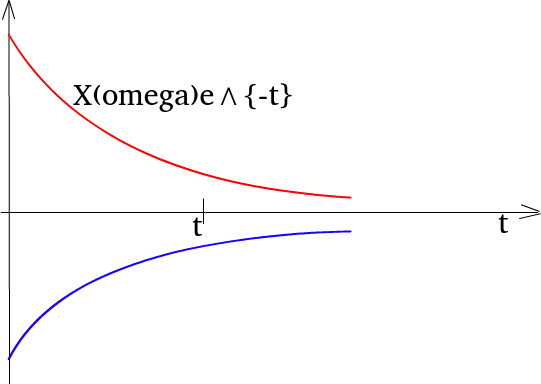
\includegraphics[width=.4\textwidth]{./pictures/2_2.png}
  \caption{Траектория процесса}
  \label{fig:22}
\end{figure}

\subsubsection*{2.3}

\textit{Задание.}
Пусть
$$ \xi \left( t \right) =
  e^{-Xt}, \,
  t > 0,$$
где $X$ --- случайная величина, которая имеет показательное распределение с параметром $ \lambda $.
Запишите конечномерные распределения случайного процесса
$ \left\{ \xi \left( t \right), \, t > 0 \right\} $.
Найдите его математическое ожидание, дисперсию и ковариационную функцию.

\textit{Решение.}
$ \xi \left( t \right) = e^{-Xt}$, где $X \sim Exp \left( \lambda \right), \, t > 0$.

Нужно найти $m \left( t \right), \, K \left( t, s \right) $, конечномерные распределения.

Найдём математическое ожидание в момент $t$.
По определению
$$m \left( t \right) =
  Me^{-Xt} =
  \int \limits_0^{+ \infty } \lambda e^{- \lambda x} e^{-Xt} dX =
  \frac{ \lambda }{ \lambda + t}.$$
Траектории такого процесса изображены на рисунке \ref{fig:23}: чем больше $X$,
тем быстрее эта функция убывает.

\begin{figure}[h!]
  \centering
  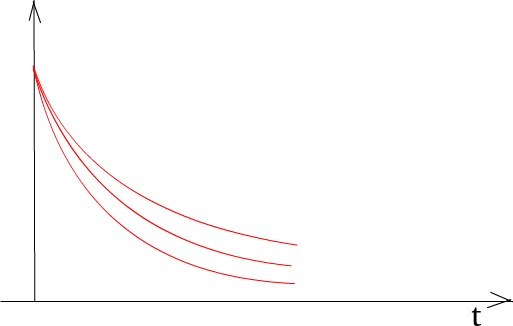
\includegraphics[width=.4\textwidth]{./pictures/2_3.png}
  \caption{Траектория процесса}
  \label{fig:23}
\end{figure}

Ковариационная функция считается по определению
$$K \left( t, s \right) =
  M \xi \left( t \right) \xi \left( s \right) - M \xi \left( t \right) M \xi \left( s \right) =
  Me^{-Xt - Xs} - \frac{ \lambda }{ \lambda + t} \cdot \frac{ \lambda }{ \lambda + s}.$$
Подставим найденное значение фунцкии математического ожидания
$$Me^{-Xt - Xs} - \frac{ \lambda }{ \lambda + t} \cdot \frac{ \lambda }{ \lambda + s} =
  \frac{ \lambda }{ \lambda + t + s} -
  \frac{ \lambda^2}{ \left( \lambda + t \right) \left( \lambda + s \right) }.$$

Считаем функцию распределения случайного вектора
$ \left( \xi \left( t_1 \right), \dotsc, \xi \left( t_n \right) \right) $ --- рис. \ref{fig:231}.

\begin{figure}[h!]
  \centering
  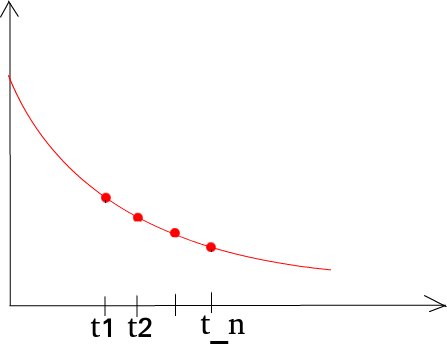
\includegraphics[width=.4\textwidth]{./pictures/2_3_1.png}
  \caption{Выбираем точки, в которых ищем распределение случайного процесса}
  \label{fig:231}
\end{figure}

$F_{ \left( \xi \left( t_1 \right), \dotsc, \xi \left( t_n \right) \right) }
  \left( \vec{x} \right) =
  P \left\{ \xi \left( t_1 \right) \leq x_1, \dotsc, \xi \left( t_n \right) \leq x_n \right\} $.
Вместо $ \xi $ напишем формулу
$P \left\{ \xi \left( t_1 \right) \leq x_1, \dotsc, \xi \left( t_n \right) \leq x_n \right\} =
  P \left( e^{-Xt_1} \leq x_1, \dotsc, e^{-Xt_n} \leq x_n \right) $.
Величины зависимы, потому что все они выражаются через $X$.
Все неравенства решаем относительно $X$
$$P \left( e^{-Xt_1} \leq x_1, \dotsc, e^{-Xt_n} \leq x_n \right) =
  P \left\{ X \geq -\frac{ln \, x_1}{t_1}, \dotsc, X \geq -\frac{ln \, x_n}{t_n} \right\}.$$
Перепишем через максимум
$$P \left\{ X \geq -\frac{ln \, x_1}{t_1}, \dotsc, X \geq -\frac{ln \, x_n}{t_n} \right\} =
  P \left\{
    X \geq \max \left( -\frac{ln \, x_1}{t_1}, \dotsc, -\frac{ln \, x_n}{t_n} \right) \right\}.$$
Обозначим максимум буквой $m$
$$P \left\{
    x \geq \max \left( -\frac{ln \, x_1}{t_1}, \dotsc, -\frac{ln \, x_n}{t_n} \right) \right\} =
  \int \limits_m^{+\infty } \lambda e^{-\lambda X} dX =
  -\left. e^{-\lambda X} \right|_m^{+\infty}.$$
На бесконечности получаем ноль
$$-\left. e^{-\lambda X} \right|_m^{+\infty} =
  e^{-\lambda m} =
  e^{-\lambda \max \left( ln \, x_1^{-\frac{1}{t_1}}, \dotsc, ln \, x_n^{-\frac{1}{t_n}} \right) }.$$
Выносим логарифм
$$e^{-\lambda \max \left( ln \, x_1^{-\frac{1}{t_1}}, \dotsc, ln \, x_n^{-\frac{1}{t_n}} \right) } =
e^{-\lambda ln \max \left( x_1^{-\frac{1}{t_1}}, \dotsc, x_n^{-\frac{1}{t_n}} \right) }.$$
Экспонента и логарифм уничтожают друг друга
$$e^{-\lambda ln \max \left( x_1^{-\frac{1}{t_1}}, \dotsc, x_n^{-\frac{1}{t_n}} \right) } =
  \max \left( x_1^{-\frac{1}{t_1}}, \dotsc, x_n^{-\frac{1}{t_n}} \right)^{-\lambda } =
  \min \left( x_1^{ \frac{ \lambda }{t_1}}, \dotsc, x_n^{ \frac{ \lambda }{t_n}} \right).$$

Все выкладки были законные, только когда $0 < x_1, \dotsc, x_n < 1$.

Плотности у такого векора $ \left( \xi \left( t_1 \right), \dotsc, \xi \left( t_n \right) \right) $
быть не может, потому что
$ \xi \left( t_1 \right)^{ \frac{1}{t_1}} =
  e^{-X} =
  \xi \left( t_2 \right)^{ \frac{1}{t_2}}$.
Сейчас у нас только одна случайная величина.
Это можно переписать как
$ \xi \left( t_2 \right) = \xi \left( t_1 \right)^{ \frac{t_2}{t_1}}, \,
  y = x^{ \frac{t_2}{t_1}}.$

С вероятностью 1 $ \left( \xi \left( t_1 \right), \xi \left( t_2 \right) \right) \in L$ ---
рис. \ref{fig:232}.

\begin{figure}[h!]
  \centering
  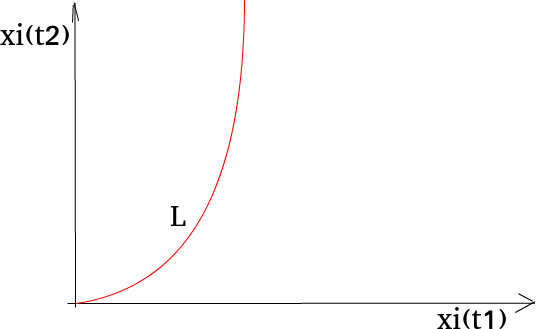
\includegraphics[width=.5\textwidth]{./pictures/2_3_2.png}
  \caption{$y = x^{ \frac{t_2}{t_1}}$}
  \label{fig:232}
\end{figure}

Значения вектора всегда попадают на такую линию.
Площадь кривой --- ноль.

Плотность --- производная от функции распределения, а минимум нельзя дифференцировать.

\subsubsection*{2.4}

\textit{Задание.}
Рассмотрим случайный процесс
$$X \left( t \right) =
  A \cos \left( \varphi + \lambda t \right),$$
где $A$ и $ \varphi $ являются независимыми случайными величинами такими, что $MA^2 < \infty $,
а $ \varphi $ имеет равномерное распределение на отрезке $ \left[ 0, 2 \pi \right] $.
Найдите математическое ожидание и ковариационную функцию процесса
$$ \left\{ X \left( t \right), \, t \geq 0 \right\}.$$

\textit{Решение.} $ \varphi \sim U \left( \left[ 0, 2 \pi \right] \right) $.

Траектория такого процесса изображена на рисунке \ref{fig:24}.

\begin{figure}[h!]
 \centering
 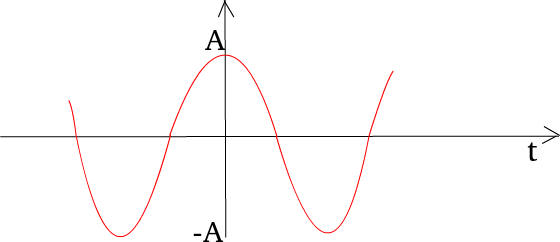
\includegraphics[width=.5\textwidth]{./pictures/2_4.png}
 \caption{Траектория процесса}
 \label{fig:24}
\end{figure}

Тут случайная амплитуда и случайный сдвиг по фазе.

$MX \left( t \right) =
M \left[ A \cos \left( \varphi + \lambda t \right) \right] $.
Случайные величины $A$ и $ \varphi $ --- независимые.
$M \left[ A \cos \left( \varphi + \lambda t \right) \right] =
  MAM \cos \left( \varphi + \lambda t \right) $.
Математическое ожидание косинуса можем найти, потому что у $ \varphi $ известна плотность
$$MAM \cos \left( \varphi + \lambda t \right) =
  MA \cdot \int \limits_0^{2 \pi }
    \cos \left( \varphi + \lambda t \right) \cdot \frac{1}{2 \pi } \cdot d \varphi.$$
Интеграл косинуса по периоду --- ноль.

Ковариационная функция
$K \left( t, s \right) =
  MX \left( t \right) X \left( s \right) - MX \left( t \right) MX \left( s \right) =$
Произведение математических ожиданий мы знаем
$$= MX \left( t \right) X \left( s \right) =
  M \left[
    A^2 \cos \left( \varphi + \lambda t \right) \cos \left( \varphi + \lambda s \right) \right] =$$
Используем независимость
$$= MA^2 \cdot
  M \left[ \cos \left( \varphi + \lambda t \right) \left( \varphi + \lambda s \right) \right] =$$
Применяем формулу для произведения косинусов
$$= MA^2 \cdot M \left\{
    \frac{1}{2} \cdot \cos \left[ 2 \varphi + \lambda \left( t + s \right) \right] +
    \frac{1}{2} \cdot \cos \left[ \lambda \left( t - s \right) \right] \right\} =$$
Математическое ожидание первого слагаемого --- ноль
$$= \frac{1}{2} \cdot MA^2 \cdot \cos \left[ \lambda \left( t - s \right) \right].$$

Двумерная характеристика процесса зависит только от расстояния между двумя точками.
Это стационарный процесс.
Его характеристики не меняются при сдвиге.

\subsubsection*{2.5}

\textit{Задание.}
Пусть $ \tau $ --- случайная величина,
которая имеет равномерное распределение на отрезке $ \left[ 0, 1 \right] $,
и пусть $ \left\{ X \left( t \right), \, t \in \left[ 0, 1 \right] \right\} $ --- процесс ожидания,
связанный с этой случайной величиной, то есть
$$X \left( t \right) =
  \mathbbm{1} \left\{ t \geq \tau \right\}, \,
  t \in \left[ 0, 1 \right].$$
Запишите конечномерные распределения процесса
$ \left\{ X \left( t \right), \, t \in \left[ 0, 1 \right] \right\} $,
найдите его математическое ожидание и ковариационную функцию.

\textit{Решение.}
$ \tau $ --- случайная величина с распределением $U \left( \left[ 0 , 1 \right] \right) $.

Сначала нарисуем траекторию такого процесса (рис. \ref{fig:25}).
Случайное $ \tau $ выпало.

\begin{figure}[h!]
 \centering
 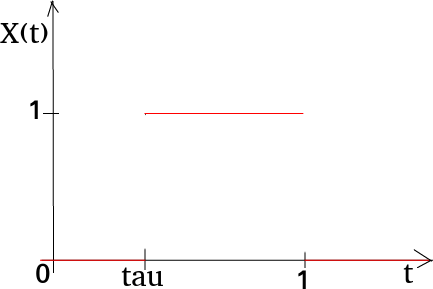
\includegraphics[width=.5\textwidth]{./pictures/2_5.png}
 \caption{Траектория процесса}
 \label{fig:25}
\end{figure}

$$m \left( t \right) =
  MX \left( t \right) =
  M \mathbbm{1} \left\{ t \geq \tau \right\} =
  P \left( t \geq \tau \right) =
  F_{ \tau } \left( t \right) =
  \frac{t - a}{b - a} =
  t.$$

Ковариационная функция
$K \left( t, s \right) =
  M \left[ X \left( t \right) X \left( s \right) \right] -
  MX \left( t \right) MX \left( s \right) $.
Произведение индикаторов --- это индикатор пересечения
$$M \left[ X \left( t \right) X \left( s \right) \right] -
  MX \left( t \right) MX \left( s \right) =
  P \left\{ \tau \leq \min \left( t, s \right) \right\} - ts =
  \min \left( t, s \right) - t \cdot s.$$

Конечномерные распределения ---
распределение вектора $ \left( X \left( t_1 \right), \dotsc, X \left( t_n \right) \right) $.
Каждый $X$ --- это 0 или 1.
$$P \left\{
    \left( X \left( t_1 \right), \dotsc, X \left( t_n \right) \right) = \left( 0, \dotsc, 0 \right)
  \right\} =
  P \left\{ \tau \in \left( t_n , 1 \right] \right\} =
  1 - t_n.$$
Точки $t_n$ изображены на рисунке \ref{fig:251}.

\begin{figure}[h!]
 \centering
 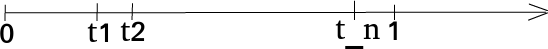
\includegraphics[width=.5\textwidth]{./pictures/2_5_1.png}
 \caption{Временная ось}
 \label{fig:251}
\end{figure}

У вектора получается $ \left( n + 1 \right) $-но значение
$$ \left( X \left( t_1 \right), \dotsc, X \left( t_n \right) \right) =
  \begin{cases}
    \left( 0, \dotsc, 0 \right), \qquad 1 - t_n, \\
    \left( 0, \dotsc, 0, 1 \right), \qquad t_n - t_{n - 1}, \\
    \dotsc, \\
    \left( 0, \dotsc, 0, 1, \dotsc, 1 \right), \qquad t_{k + 1} - t_k, \\
    \dotsc, \\
    \left( 1, \dotsc, 1 \right), \qquad t_1.
  \end{cases}$$

\subsubsection*{2.6}

\textit{Задание.}
Пусть $ \xi_1, \xi_2, \dotsc, \xi_n$ ---
независимые одинаково распределённые случайные величины с функцией распределения $F$, и пусть
$$X \left( t \right) \equiv
  F_n^* \left( t \right) =
  \frac{1}{n} \sum \limits_{i = 1}^n \mathbbm{1} \left\{ \xi_i \leq t \right\}, \,
  t \in \mathbb{R}.$$
Запишите конечномерные распределения процесса
$ \left\{ X \left( t \right), \, t \in \mathbb{R} \right\} $,
найдите его математическое ожидание и ковариационную функцию.

\textit{Решение.}
$$X \left( t \right) =
  \frac{1}{n} \sum \limits_{i = 1}^n \mathbbm{1} \left\{ \xi_i \leq t \right\} $$
--- это эмпирическая функция распределения (рис. \ref{fig:26}).

\begin{figure}[h!]
 \centering
 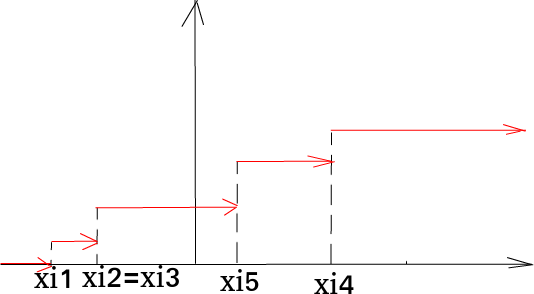
\includegraphics[width=.5\textwidth]{./pictures/2_6.png}
 \caption{Эмпирическая функция распределения}
 \label{fig:26}
\end{figure}

Эмпирическая функция распределения --- это несмещённая оценка функции распределения.

$$cov \left( X \left( t \right), X \left( s \right) \right) =
  cov \left(
    \frac{1}{n} \sum \limits_{i = 1}^n \mathbbm{1} \left\{ \xi_i \leq t \right\}, \,
    \frac{1}{n} \sum \limits_{i = 1}^n \mathbbm{1} \left\{ \xi_i \leq s \right\} \right) =$$
Нужно вынести константы
$$= \frac{1}{n^2}
  \sum \limits_{i,j=1}^n
    cov \left(
      \mathbbm{1} \left\{ \xi_i \leq t, \, \mathbbm{1} \left\{ \xi_j \leq s \right\} \right\}
    \right) =$$
Случайные величины $ \xi_1, \dotsc, \xi_n$ --- независимые.
Ковариация независимых величин --- ноль
$$= \frac{1}{n^2}
  \sum \limits_{i = 1}^n
    \left(
      \mathbbm{1} \left\{ \xi_i \leq t \right\}, \, \mathbbm{1} \left\{ \xi_i \leq s \right\}
    \right).$$

Посчитаем ковариацию двух индикаторов
$$cov \left(
    \mathbbm{1} \left\{ \xi_i \leq t \right\}, \, \mathbbm{1} \left\{ \xi_i \leq s \right\}
  \right) =
  M \mathbbm{1} \left\{ \xi_i \leq t \wedge s \right\} - F \left( t \right) F \left( s \right) =$$
Математическое ожидание индикатора событие --- вероятность этого события,
которая в данном случае по определению равна функции распределения
$$= F \left( t \wedge s \right) - F \left( t \right) F \left( s \right),$$
где $ \wedge $ означает минимум.

Все слагаемые в сумме раны этому выражению
$$K \left( t, s \right) =
  \frac{1}{n} \left[ F \left( t \wedge s \right) - F \left( t \right) F \left( s \right) \right].$$

Теперь нужно написать конечномерные распределения этого процесса.
Фиксируем $t_1, t_2, \dotsc, t_m$ (рис. \ref{fig:261}).

$$X \left( t \right) \in
  \left\{ 0, \frac{1}{n}, \frac{2}{n}, \dotsc, 1 \right\}.$$

По $t, \, X$ увеличивается.
Эта функция монотонна.

\begin{figure}[h!]
 \centering
 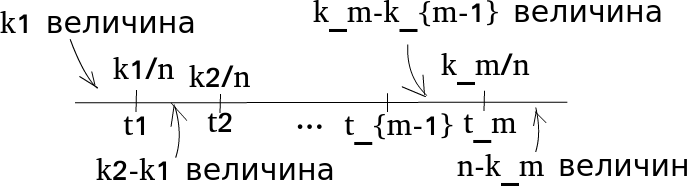
\includegraphics[width=.5\textwidth]{./pictures/2_6_1.png}
 \caption{Фиксируем моменты времени}
 \label{fig:261}
\end{figure}

$0 \leq k_1 \leq k_2 \leq \dotsc \leq k_m \leq n$.

Конечномерные распределения имеют вид
$$P \left\{
    X \left( t_1 \right) = \frac{k_1}{n}, \,
    X \left( t_2 \right) = \frac{k_2}{n}, \dotsc, X \left( t_m \right) = \frac{k_m}{n} \right\} =$$
$P$(для $k_1$ наблюдений $ \xi \leq t_1$, для $k_2 - k_1$ наблюдений $t_1 < \xi \leq t_2, \dotsc,$
для $n - k_m$ наблюдений $ \xi > t_m$)
Имеем мультиномиальное распределение
$$= \frac{n!}{k_1! \left( k_2 - k_1 \right)! \dotsc \left( n - k_m \right)!} \cdot
  F \left( t_1 \right)^{k_1} \cdot
  \left[ F \left( t_2 \right) - F \left( t_1 \right) \right]^{k_2 - k_1} \cdot \dotsc,$$
где первое слагаемое --- количество способов разбить $n$ величин на группы.

\subsubsection*{2.7}

\textit{Задание.}
Найдите характеристическую функцию случайной величины $X \left( \eta \right) $,
где $ \left\{ X \left( t \right), \, t \in \left[ 0, 1 \right] \right\} $ --- процесс из задачи 2.5,
а $ \eta $ --- независимая от $X$ случайная величина,
которая принимает значения 0 и 1 с вероятностями $ \frac{1}{3}$ и $ \frac{2}{3}$ соответственно.

\textit{Решение.}
$X \left( t \right) =
  \mathbbm{1} \left\{ t \geq \tau \right\} $.

Задана случайная величина
$$ \eta =
  \begin{cases}
    0, \qquad \frac{1}{3}, \\
    1, \qquad \frac{2}{3}.
  \end{cases}$$

Интересуемся $ \varphi_{X \left( \eta \right) }$.
Траектория случайного процесса изображён на рисунке \ref{fig:27}.

\begin{figure}[h!]
 \centering
 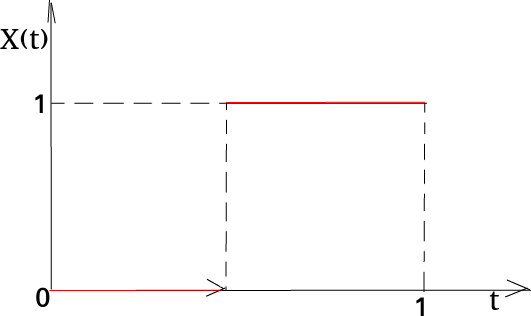
\includegraphics[width=.5\textwidth]{./pictures/2_7.png}
 \caption{Траектория случайного процесса}
 \label{fig:27}
\end{figure}

Случайная величина принимает значения 0 и 1: $X \left( 0 \right) = 0, \, X \left( 1 \right) = 1$,
значит, $X \left( \eta \right) = \eta $.

$$ \varphi_{X \left( \eta \right) } \left( \lambda \right) =
  \varphi_{ \eta } \left( \lambda \right) =
  Me^{i \lambda \eta } =
  \frac{1}{3} \cdot 1 + \frac{2}{3} \cdot e^{i \lambda }.$$

То, что они независимы, тут не важно.

\addcontentsline{toc}{section}{Домашнее задание}
\section*{Домашнее задание}

\subsubsection*{2.12}

\textit{Задание.}
Пусть
$$ \xi \left( t \right) =
  Xt + a, \,
  t \in \mathbb{R},$$
где $X$ --- равномерно распределённая на отрезке $ \left( a, b \right) $ случайная величина.
Запишите конечномерные распределения случайного процесса
$ \left\{ \xi \left( t \right), \, t \in \mathbb{R} \right\} $.
Найдите его математическое ожидание, дисперсию и ковариационную функцию.

\textit{Решение.}
$ \xi \left( t \right) = Xt + a, \, t \in \mathbb{R}$, где $X \sim U \left( a, b \right) $.

Нужно найти $m \left( t \right), \, D \xi \left( t \right), \, K \left( t, s \right) $,
конечномерные распределения.

Найдём математическое ожидание в момент $t$
$$m \left( t \right) =
  M \xi \left( t \right) =
  M \left( Xt + a \right) =
  M \left( Xt \right) + Ma =
  tMX + a =
  t \cdot \frac{a + b}{2} + a.$$

Траектории такого процесса изоражены на рисунке \ref{fig:212}: чем больше $X$,
тем больше угол наклона прямой к оси $0t$.

\begin{figure}[h!]
 \centering
 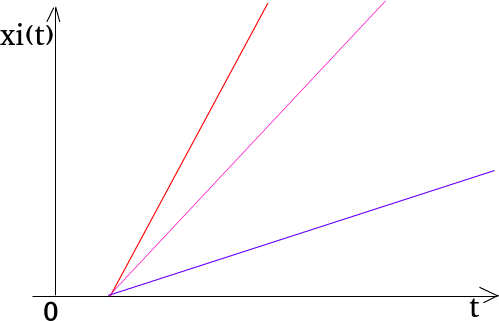
\includegraphics[width=.5\textwidth]{./pictures/2_12.png}
 \caption{Траектории случайного процесса}
 \label{fig:212}
\end{figure}

$$D \xi \left( t \right) =
  D \left( Xt + a \right) =
  D \left( Xt \right) + Da =
  t^2 DX =
  t^2 \cdot \frac{ \left( b - a \right)^2}{12}.$$

Ковариационная функция считается по определению
$$K \left( t, s \right) =
  M \left[ \xi \left( t \right) \xi \left( s \right) \right] -
  M \xi \left( t \right) M \xi \left( s \right) =$$
Подставляем выражение для случайного процесса, раскрываем скобки и вычисляем математическое ожидание
\begin{equation*}
  \begin{split}
    = M \left[ \left( Xt + a \right) \left( Xs + a \right) \right] -
    M \left( Xt + a \right) M \left( Xs + a \right) = \\
    = M \left[ X^2 ts + Xa \left(t + s \right) + a^2 \right] -
    \left( t \cdot \frac{a + b}{2} + a \right) \left( s \cdot \frac{a + b}{2} + a \right) = \\
    = ts \cdot \frac{a^2 + ab + b^2}{3} + a \left( t + s \right) \cdot \frac{a + b}{2} + a^2 -
    ts \cdot \frac{ \left( a + b \right)^2}{4} - ta \cdot \frac{a + b}{2} - a^2 - \\
    - as \cdot \frac{a + b}{2} = \\
    = ts \left( \frac{a^2 + ab + b^2}{3} - \frac{a^2 + 2ab + b^2}{4} \right) +
    \left(t + s \right) a \cdot \frac{a + b}{2} - \frac{a + b}{2} \cdot a \left( t + s \right) = \\
    = ts \cdot \frac{4a^2 + 4ab + 4b^2 - 3a^2 - 6ab - 3b^2}{12} =
    ts \cdot \frac{a^2 - 2ab + b^2}{12} =
    ts \cdot \frac{ \left( a - b \right)^2}{12}.
  \end{split}
\end{equation*}

Считаем функцию распределения случайного вектора
$ \left( \xi \left( t_1 \right), \dotsc, \xi \left( t_n \right) \right) $ --- рис. \ref{fig:2121}.

\begin{figure}[h!]
 \centering
 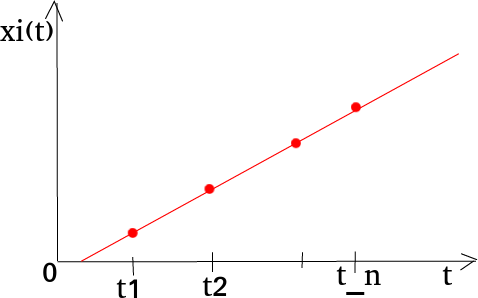
\includegraphics[width=.5\textwidth]{./pictures/2_12_1.png}
 \caption{Выбираем точки, в которых ищем распределение случайного процесса}
 \label{fig:2121}
\end{figure}

$F_{ \left( \xi \left( t_1 \right), \dotsc, \xi \left( t_n \right) \right) }
  \left( \vec{x} \right) =
  P \left\{ \xi \left( t_1 \right) \leq x_1, \dotsc, \xi \left( t_n \right) \leq x_n \right\} $.
Вместо $ \xi $ напишем формулу
$P \left\{ \xi \left( t_1 \right) \leq x_1, \dotsc, \xi \left( t_n \right) \leq x_n \right\} =
  P \left( Xt_1 + a \leq x_1, \dotsc, Xt_n + a \leq x_n \right) $.
Величины зависимы, потому что все они выражаются через $X$.
Все неравенства решаем относительно $X$
$$P \left( Xt_1 + a \leq x_1, \dotsc, Xt_n + a \leq x_n \right) =
  P \left( Xt_1 \leq x_1 - a, \dotsc, Xt_n \leq x_n - a \right) =$$
Делим на константы левые части неравенств
$$= P \left( X \leq \frac{x_1 - a}{t_1}, \dotsc, X \leq \frac{x_n - a}{t_n} \right) =$$
Перепишем через минимум
$$= P \left\{
    X \leq \min \left( \frac{x_1 - a}{t_1}, \dotsc, \frac{x_n - a}{t_n} \right)
  \right\} =$$
Обозначим минимум буквой $m$ для удобства
$$= P \left( X \leq m \right) =
  \int \limits_a^m \frac{1}{b - a} \cdot \mathbbm{1} \left\{ X \in \left( a, b \right) \right\} dX =
  \frac{1}{b - a} \int \limits_a^m dX =
  \frac{1}{b - a} \cdot \left. X \right|_a^m =$$
Подставляем пределы интегрирования
$$= \frac{1}{b - a} \cdot \left( m - a \right) =
  \frac{1}{b - a} \cdot
  \left[ \min \left( \frac{x_1 - a}{t_1}, \dotsc, \frac{x_n - a}{t_n} \right) - a \right] $$
при $m \in \left( a, b \right) $, иначе --- ноль.

\subsubsection*{2.13}

\textit{Задание.}
Пусть
$$ \xi \left( t \right) =
  U \cos \theta t + V \sin \theta t, \,
  t \in T,$$
где $U, V$ --- независимые случайные величины с заданными характеристиками:
$MU = MV = 0, \, DU = DV = \sigma^2, \, \theta $ --- неслучайная величина.
Найдите математическое ожидание, дисперсию и ковариационную функцию случайного процесса
$ \left\{ \xi \left( t \right), \, t \in T \right\} $.

\textit{Решение.}
Нужно найти $m \left( t \right), \, D \xi \left( t \right), \, K \left( t, s \right) $.

Найдём математическое ожидание в момент $t$.
По свойствам
$$m \left( t \right) =
  M \xi \left( t \right) =
  M \left( U \cos \theta t + V \sin \theta t \right) =
  \cos \theta t \cdot MU + \sin \theta t \cdot MV =
  0.$$

Можно сделать преобразование
$U \cos \theta t + V \sin \theta t = C \sin \left( \theta t + \omega \right) $,
где $C = \sqrt{U^2 + V^2}$.
Траектории такого процесса изображены на рисунке \ref{fig:213}:
график синуса сжимается к оси ординат, когда модули случайных величин $U$ и $V$ растут.

\begin{figure}[h!]
 \centering
 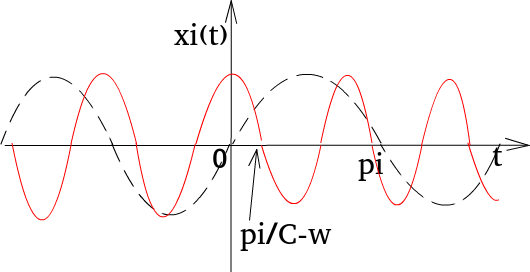
\includegraphics[width=.5\textwidth]{./pictures/2_13.png}
 \caption{Траектория процесса}
 \label{fig:213}
\end{figure}

Найдём дисперсию в момент $t$.
По свойствам
$$D \xi \left( t \right) =
  D \left( U \cos \theta t + V \sin \theta t \right) =
  \cos^2 \theta  t \cdot DU + \sin^2 \theta t \cdot DV =$$
Подставим известные значения дисперсии
$$= \cos^2 \theta t \cdot \sigma^2 + \sin^2 \theta t \cdot \sigma^2 =
  \sigma^2 \left( \cos^2 \theta t + \sin^2 \theta t \right) =
  \sigma^2.$$

Ковариационная функция считается по определению
$$K \left( t, s \right) =
  M \xi \left( t \right) \xi \left( s \right) - M \xi \left( t \right) M \xi \left( s \right) =$$
Подставим выражения для случайного процесса в первое слагаемое, а второе равно нулю
$$= M \left[ \left( U \cos \theta t + V \sin \theta t \right) \cdot
    \left( U \cos \theta s + V \sin \theta s \right) \right] =$$
Раскроем скобки
\begin{equation*}
  \begin{split}
    = M(
      U^2 \cos \theta t \cdot \cos \theta s + UV \cos \theta t \cdot \sin \theta s +
      VU \sin \theta t \cdot \cos \theta
       s + \\
      + V^2 \sin \theta t \cdot \sin \theta s) = \\
    = DU \cdot \cos \theta t \cdot \cos \theta s +
    MU \cdot MV \cdot \cos \theta t \cdot \sin \theta s +
    MV \cdot MU \cdot \sin \theta t \cdot \cos \theta s + \\
    + DV \cdot \sin \theta t \cdot \sin \theta s =
    \sigma^2 \cos \theta t \cdot \cos \theta s + \sigma^2 \sin \theta t \cdot \sin \theta s = \\
    = \sigma^2 \cdot
      \left( \cos \theta t \cdot \cos \theta s + \sin \theta t \cdot \sin \theta s \right) =
    \sigma^2 \cos \left( \theta t - \theta s \right) =
    \sigma^2 \cos \left[ \theta \left( t - s \right) \right].
  \end{split}
\end{equation*}

\subsubsection*{2.14}

\textit{Задание.}
Определите математическое ожидание, дисперсию и ковариационную функцию процесса
$$ \xi \left( t \right) =
  2u \sin \nu t + 3vt^2 + 5, \,
  t \in T,$$
где $ \nu $ --- известный неслучайный параметр, а $u, v$ ---
случайные величины с известными характеристиками:
$$Mu = 1, \,
  Mv = 2, \,
  Du = 0.1, \,
  Dv = 0.9, \,
  cov \left( u, v \right) = -0.3.$$

\textit{Решение.}
Нужно найти $m \left( t \right), \, D \xi \left( t \right), \, K \left( t, s \right) $.

Найдём математическое ожидание в момент $t$.
По свойствам
$$m \left( t \right) =
  M \left( 2u \sin \nu t + 3vt^2 + 5 \right) =
  2 \sin \nu t \cdot Mu + 3t^2 Mv + 5 =
  2 \sin \nu t + 6t^2 + 5.$$

Траектория такого процесса изображена на рисунке \ref{fig:214}.

\begin{figure}[h!]
 \centering
 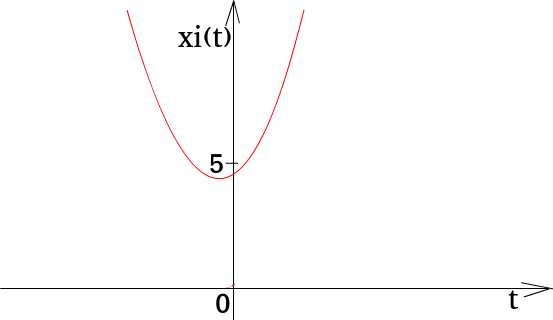
\includegraphics[width=.5\textwidth]{./pictures/2_14.png}
 \caption{Траектория процесса}
 \label{fig:214}
\end{figure}

Ковариационная функция считается по определению
$$K \left( t, s \right) =
  M \xi \left( t \right) \xi \left( s \right) -
    M \xi \left( t \right) \cdot M \xi \left( s \right) =$$
Подставим выражения для случайного процесса и его математические ожидания
\begin{equation*}
  \begin{split}
    = M \left[
      \left( 2u \sin \nu t + 3vt^2 + 5 \right) \left( 2u \sin \nu s + 3vs^2 + 5 \right) \right] - \\
    - \left( 2 \sin \nu t + 6t^2 + 5 \right) \left( 2 \sin \nu s + 6s^2 + 5 \right) = \\
    = M(4u^2 \sin \nu t \cdot \sin \nu s + 6uv \sin \nu t \cdot s^2 + 10u \sin \nu t +
      6vt^2 u \sin \nu s + 9v^2 t^2 s^2 + \\
      + 15vt^2 + 10u \sin \nu s + 15vs^2 + 25) -
    4 \sin \nu t \cdot \sin \nu s - 12 \sin \nu t \cdot s^2 - 10 \sin \nu t - \\
    - 12t^2 \sin \nu s - 36t^2 s^2 - 30t^2 - 10 \sin \nu s - 30s^2 - 25 = \\
    = 4 \sin \nu t \cdot Mu^2 + 6t^2 \sin \nu s \cdot M \left( uv \right) + 10 \sin \nu t \cdot Mu +
    6t^2 \sin \nu s \cdot M \left( uv \right) + \\
    + 9t^2 s^2 Mv^2 + 15t^2 Mv + 10 \sin \nu s \cdot Mu + 15s^2 \cdot Mv + 25 -
    4 \sin \nu t \cdot \sin \nu s - \\
    - 12 \sin \nu t \cdot s^2 - 10 \sin \nu t - 12t^2 \sin \nu s - 36t^2 s^2 - 30t^2 -
    10 \sin \nu s - 30s^2 - 25 =
  \end{split}
\end{equation*}
Вычислим вторые моменты
$$Mu^2 = Du + \left( Mu \right)^2 = 0.1 + 1 = 1.1, \,
  Mv^2 = Dv + \left( Mv \right)^2 = 0.9 + 4 = 4.9.$$
По определению ковариации $cov \left( u, v \right) = M \left( uv \right) - Mu \cdot Mv$,
откуда
$$M \left( uv \right) =
  cov \left( u, v \right) + Mu \cdot Mv =
  -0.3 + 1 \cdot 2 =
  2 - 0.3 =
  1.7.$$
Подставим полученные значения в функцию ковариации
\begin{equation*}
  \begin{split}
    = 4 \sin \nu t \cdot \sin \nu s \cdot 1.1 + 6 \sin \nu t \cdot s^2 \cdot 1.7 + 10 \sin \nu t +
    6t^2 \sin \nu s \cdot 1.7 + \\
    + 9t^2 s^2 \cdot 4.9 + 15t^2 \cdot 2 + 10 \sin \nu s + 15s^2 \cdot 2 -
    4 \sin \nu t \cdot \sin \nu s - 12 \sin \nu t \cdot s^2 - \\
    - 10 \sin \nu t - 12t^2 \cdot \sin \nu s - 36t^2 s^2 - 30t^2 - 10 \sin \nu s - 30s^2 = \\
    = 0.4 \sin \nu t \cdot \sin \nu s - 1.8 \sin \nu t \cdot s^2 - 1.8t^2 \sin \nu s + 8.1t^2 s^2.
  \end{split}
\end{equation*}

Найдём дисперсию в момент $t$.
Из формулы для ковариации
$$D \xi \left( t \right) =
  K \left( t, t \right) =
  0.4 \sin^2 \nu t - 3.6 \sin \nu t \cdot t^2 + 8.1t^4.$$

\subsubsection*{2.15}

\textit{Задание.}
Найдите ковариационную функцию процесса
$$Y \left( t \right) =
  \psi_1 \left( t \right) X_1 + \dotsc + \psi_n \left( t \right) X_n,$$
где $ \psi_1, \dotsc, \psi_n$ --- произвольные числовые функции от $t$, а $X_1, \dotsc, X_n$ ---
некоррелируемые случайные величины с дисперсиями $D_1, \dotsc, D_n$.

\textit{Решение.}
Нужно найти
$$K \left( t, s \right) =
  cov \left( \psi_1 \left( t \right) X_1 + \dotsc + \psi_n \left( t \right) X_n, \,
    \psi_1 \left( s \right) X_1 + \dotsc + \psi_n \left( s \right) X_n \right) =$$
Распишем по определению
\begin{equation*}
  \begin{split}
    = M \left[
      \left( \psi_1 \left( t \right) X_1 + \dotsc + \psi_n \left( t \right) X_n \right)
      \left( \psi_1 \left( s \right) X_1 + \dotsc + \psi_n \left( s \right) X_n \right) \right] - \\
    - M \left( \psi_1 \left( t \right) X_1 + \dotsc + \psi_n \left( t \right) X_n \right) \cdot
    M \left( \psi_1 \left( s \right) X_1 + \dotsc + \psi_n \left( s \right) X_n \right) = \\
    = \sum \limits_{i, j = 1}^n
      \psi_i \left( t \right) \psi_j \left( s \right) M \left( X_i X_j \right) -
    \sum \limits_{i, j = 1}^n \psi_i \left( t \right) \psi_j \left( s \right) MX_i \cdot MX_j = \\
    = \psi_1 \left( t \right) \psi_1 \left( s \right) DX_1 + \dotsc +
    \psi_n \left( t \right) \psi_n \left( s \right) DX_n= \\
    = \psi_1 \left( t \right) \psi_1 \left( s \right) D_1 + \dotsc +
    \psi_n \left( t \right) \psi_n \left( s \right) D_n.
  \end{split}
\end{equation*}

\subsubsection*{2.16}

\textit{Задание.}
Пусть $ \eta $ и $ \zeta $ --- независимые нормально распределённые
случайные величины с нулевым математическим ожиданием и дисперсиями $1 / 2$.
Найдите конечномерные распределения случайного процесса
$$ \xi \left( t \right) =
  \frac{ \eta + \zeta }{t}, \,
  t > 0.$$

\textit{Решение.}
Для произвольных натуральных $n \geq 1$,
произвольных моментов времени $t_1, \dotsc, t_n \in T$ и произвольных действительных чисел
$x_1, \dotsc, x_n$ находим
$$F_{t_1, t_2, \dotsc, t_n} \left( x_1, x_2, \dotsc, x_n \right) =
  P \left\{
    \xi \left( t_1 \right) \leq x_1, \xi \left( t_2 \right) \leq x_2, \dotsc,
    \xi \left( t_n \right) \leq x_n \right\} =$$
Подставляем выражения для случайного процесса
$$= P \left(
    \frac{ \eta + \zeta }{t_1} \leq x_1, \frac{ \eta + \zeta }{t_2} \leq x_2, \dotsc,
    \frac{ \eta + \zeta }{t_n} \leq x_n \right) =$$
Переносим моменты времени вправо
$$= P \left(
    \eta + \zeta \leq x_1 t_1, \eta + \zeta \leq x_2 t_2, \dotsc, \eta + \zeta \leq x_n t_n
  \right) =$$
Независимые случайные величины $ \eta $ и $ \zeta $ имеют нормальное распределение с параметрами
$a = 0$ и
$$ \sigma^2 =
  \frac{1}{2}.$$
Их сумма имеет стандартное нормальное распределение.
Пусть
$$ \eta + \zeta =
  X \sim
  N \left( 0, 1 \right).$$
Тогда
$$= P \left( X \leq x_1 t_1, X \leq x_2 t_2, \dotsc, X \leq x_n t_n \right) =
  P \left( X \leq \min \limits_{i = \overline{1, n}} x_i t_i \right) =$$
Запишем через плотность
$$= \int \limits_{- \infty }^z \frac{1}{ \sqrt{2 \pi }} \cdot e^{- \frac{y^2}{2}} dy,$$
где обозначено
$$z =
  \min \limits_{i = \overline{1, n}} x_i t_i.$$

\subsubsection*{2.17}

\textit{Задание.}
Найдите характеристическую функцию случайной величины $ \xi \left( \tau \right) $,
где $ \left\{ \xi \left( t \right),\ , t \geq 0 \right\} $ --- процесс из предыдущей задачи,
а $ \tau $ --- независимая от $ \xi $ случайная величина,
которая принимает значения $+1$ и $-1$ с вероятностями $1 / 2$.

\textit{Решение.}
$$ \xi \left( t \right) =
  \frac{ \eta + \zeta }{t}.$$

Задана случайная величина
$$ \tau =
  \begin{cases}
    1, \qquad \frac{1}{2}, \\
    -1, \qquad \frac{1}{2}.
  \end{cases}$$

Интересует
$$ \varphi_{ \xi \left( \tau \right) } \left( \lambda \right) =
  Me^{i \xi \left( \tau \right) \lambda } =
  Me^{i \cdot \frac{ \eta + \zeta }{ \tau } \cdot \lambda } =$$
Как и в предыдущей задаче $ \eta + \zeta = X \sim N \left( 0, 1 \right) $.
Получаем
$$= Me^{i \cdot \frac{X}{ \tau } \cdot \lambda } =
  Me^{-\frac{ \lambda ^2}{2 \tau^2}} =
  e^{- \frac{ \lambda^2}{2}}.$$

\addcontentsline{toc}{chapter}{Занятие 3. Процесс Пуассона}
\chapter*{Занятие 3. Процесс Пуассона}

\addcontentsline{toc}{section}{Контрольные вопросы и задания}
\section*{Контрольные вопросы и задания}

\subsubsection*{Приведите определение процесса Пуассона.}

$\left\{ N \left( t \right), \, t \geq 0 \right\} $ --- процесс Пуассона, если
\begin{enumerate}
  \item $N \left( 0 \right) = 0$;
  \item при $t_1 < t_2 < \dotsc < t_n$ события
  $$N \left( t_1 \right), N \left( t_2 \right) - N \left( t_1 \right), \dotsc,
    N \left( t_n \right) - N \left( t_{n - 1} \right) $$
  --- независимые;
  \item число событий на интервале зависит только от длины интервала,
  то есть есть однородность приращений
  $$N \left( t + s \right) - N \left( t \right) \overset{d}{=}
    N \left( s \right) \sim
    Pois \left( \lambda s \right).$$
\end{enumerate}

\subsubsection*{Запишите конечномерные распределения процесса Пуассона.}

Одномерные распределения
$$P \left\{ N \left( t \right) = k \right\} =
  e^{-\lambda t} \cdot \frac{ \left( \lambda t \right)^k}{k!}.$$

Двумерные распределения: $t_1 < t_2$.
Перейдём к приращениям
$$P \left\{ N \left( t_1 \right) = k_1, \, N \left( t_2 \right) = k_2 \right\} =
  P \left\{
    N \left( t_1 \right) = k_1, \, N \left( t_2 \right) - N \left( t_1 \right) = k_2 - k_1
  \right\} =$$
Случайная величина $N \left( t_1 \right) \sim Pois \left( \lambda t_1 \right) $, а
$N \left( t_2 \right) - N \left( t_1 \right) \sim
  Pois \left( \lambda \left( t_2 - t_1 \right) \right) $.
Совместная вероятность --- это произведение вероятностей
$$= e^{-\lambda t_1} \cdot \frac{ \left( \lambda t_1 \right)^{k_1}}{k_1!} \cdot
  e^{-\lambda \left( t_2 - t_1 \right) } \cdot
  \frac{ \left( \lambda \left( t_2 - t_1 \right) \right)^{k_2 - k_1}}{ \left( k_2 - k_1 \right)!}.$$

\subsubsection*{Какой вид имеют траектории процесса Пуассона?}

Траектория изображена на рисунке \ref{fig:3}.

\begin{figure}[h!]
  \centering
  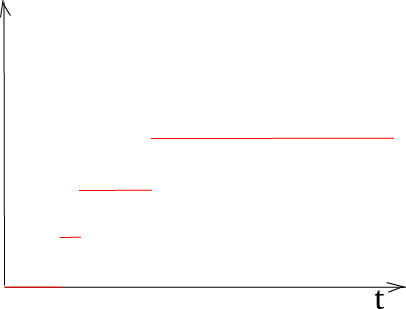
\includegraphics[width=.4\textwidth]{./pictures/3.png}
  \caption{График пуассоновского процесса}
  \label{fig:3}
\end{figure}

\subsubsection*{Какое содержание имеет параметр процесса Пуассона?}

$N \left( t \right) $ --- число событий, произошедших до момента времени $t$.

\addcontentsline{toc}{section}{Аудиторные задачи}
\section*{Аудиторные задачи}

\subsubsection*{3.2}

\textit{Задание.}
Пусть $ \left\{ N \left( t \right), \, t \geq 0 \right\} $ ---
процесс Пуассона с интенсивностью
$$ \lambda = 2.$$
Вычислите вероятности:
\begin{enumerate}[label=\alph*)]
  \item $P \left( N \left( 6 \right) = 3 \right) $;
  \item $P \left(
    N \left( 6 \right) = 3, \, N \left(9 \right) = 7, \, N \left( 15 \right) = 10 \right) $;
  \item $P \left( N \left( 6 \right) = 3 \; \middle| \; N \left( 9 \right) = 7 \right) $;
  \item $P \left( N \left( 9 \right) = 7 \; \middle| \; N \left( 6 \right) = 3 \right) $.
\end{enumerate}

\textit{Решение.}
\begin{enumerate}[label=\alph*)]
  \item $N \left( 6 \right) \sim Pois \left( 6 \cdot 2 \right) $, поэтому
  $$P \left( N \left( 6 \right) = 3 \right) =
    \frac{12^3}{3!} \cdot e^{-12};$$
  \item нужно перейти к приращениям, потому что они независимы
  \begin{gather*}
    P \left(
      N \left( 6 \right) = 3, \, N \left(9 \right) = 7, \, N \left( 15 \right) = 10 \right) = \\
    = P \left\{
      N \left( 6 \right) = 3, \, N \left( 9 \right) - N \left( 6 \right) = 4, \,
      N \left( 15 \right) - N \left( 9 \right) = 3 \right\} = \\
    = \left( \frac{12^3}{3!} \cdot e^{-12} \right) \cdot
    \left( \frac{6^4}{4!} \cdot e^{-6} \right) \cdot \left( \frac{12^3}{3!} \cdot e^{-12} \right);
  \end{gather*}
  \item по определению условной вероятности
  \begin{gather*}
    P \left( N \left( 6 \right) = 3 \; \middle| \; N \left( 9 \right) = 7 \right) =
    \frac{P \left( N \left( 6 \right) = 3, \, N \left( 9 \right) = 7 \right) }{P \left( N \left( 9 \right) = 7 \right) } = \\
    = \frac{ \frac{12^3}{3!} \cdot e^{-12} \cdot \frac{6^4}{4!} \cdot e^{-6}}{ \frac{18^7}{7!} \cdot e^{-18}} =
    \frac{12^3 \cdot 6^4 \cdot 7!}{3! \cdot 4! \cdot 18^7};
  \end{gather*}
  \item аналогично предыдущему пункту
  \begin{gather*}
    P \left( N \left( 9 \right) = 7 \; \middle| \; N \left( 6 \right) = 3 \right) =
    \frac{P \left( N \left( 9 \right) = 7, \, N \left( 6 \right) = 3 \right) }{P \left( N \left(6 \right) = 3 \right) } = \\
    = \frac{ \frac{12^3}{3!} \cdot e^{-12} \cdot \frac{6^4}{4!} \cdot e^{-6}}{ \frac{12^3}{3!} \cdot e^{-12}} =
    \frac{6^4}{4!} \cdot e^{-6} =
    \frac{P \left( N \left( 6 \right) = 3 \right) P \left( N \left( 3 \right) = 4 \right) }{P \left( N \left( 6 \right) = 3 \right) }.
  \end{gather*}
\end{enumerate}

\subsubsection*{3.3}

\textit{Задание.}
Пусть $ \left\{ N \left( t \right), \, t \geq 0 \right\} $ ---
процесс Пуассона с интенсивностью $ \lambda $.
Вычислите условное математическое ожидание
$M \left[ N \left( s \right) \; \middle| \; N \left( t \right) \right] $ для
$$0 \leq s \leq t.$$

\textit{Решение.}
Что ж такое условное математическое ожидание?

$N \left( s \right) $ и $N \left( t \right) $ --- дискретные величины, то есть
$$M \left[ N \left( s \right) \; \middle| \; N \left( t \right) \right] =
  \sum \limits_{l = 0}^{ \infty }
    l \cdot P \left\{ N \left( s \right) = l \; \middle| \; N \left( t \right) = k \right\}.$$
Отдельно посчитаем условную вероятность, а потом по ней возьмём математическое ожидание
$$P \left\{ N \left( s \right) = l \; \middle| \; N \left( t \right) = k \right\} =
  \frac{P \left\{ N \left( t \right) - N \left( s \right) = k - l \right\} P \left\{ N \left( s \right) = l \right\} }{P \left\{ N \left( t \right) = k \right\} } =$$
подставляем пуассоновские вероятности
$$= \frac{ \frac{ \left[ \lambda \left( t - s \right) \right]^{k - l}}{ \left( k - l \right)!} \cdot e^{-\lambda \left( t - s \right) }}{ \frac{ \left( \lambda t \right)^k}{k!} \cdot e^{-\lambda t}} \cdot
  \frac{ \left( \lambda s \right)^l}{l!} \cdot e^{-\lambda l} =
  \frac{k! \left( t - s \right)^{k - l} s^l}{ \left( k - l \right)! l! t^k} =
  C_k^l \cdot \left( \frac{t - s}{t} \right)^{k - l} \cdot \left( \frac{s}{t} \right)^l.$$
Имеем биномиальное распределение с параметрами $k$ и $ \frac{s}{t}$.

Вывод: при условии $N \left( t \right) = k$ мы нашли распределение
$$N \left( s \right) \sim
  B \left( k, \frac{s}{t} \right).$$

Условное математическое ожидание
$$M \left[ N \left( s \right) \; \middle| N \left( t \right) = k \right] =
  \frac{ks}{t}.$$

Ответ: $ \frac{N \left( t \right) \cdot s}{t}$.
Куда пропала сумма?

$$M \left[ N \left( s \right) \; \middle| \; N \left( t \right) = k \right] =
  \sum \limits_l
    l \cdot P \left[ N \left( s \right) = l \; \middle| \; N \left( t \right) = k \right] =$$
Нашли эту вероятность
$$= \sum \limits_l l \cdot P \left\{ Bin \left( k, \frac{s}{t} \right) = l \right\} =
MBin \left( k, \frac{s}{t} \right) =
k \cdot \frac{s}{t}.$$

Условное математическое ожидание --- это математическое ожидание по условному распределению.

\subsubsection*{3.4}

\textit{Задание.}
Пусть $N = \left\{ N \left( t \right), \, t \geq 0 \right\} $ ---
процесс Пуассона с интенсивностью $ \lambda $.
Найдите вероятность того, что первый прыжок процесса $N$ произошёл до момента времени
$s \in \left[ 0, t \right] $ при условии,
что на отрезке $ \left[ 0, t \right] $ произошло ровно $n$ прыжков.

\textit{Решение.}
Нужно найти вероятность $P$(первый прыжок произошёл до момента
$\left. s \in \left[ 0, t \right] \right| N \left( t \right) = n$).
Нужно это условие переписать через пуассоновский процесс.
Получаем
$P$(первый прыжок произошёл до момента
  $\left. s \in \left[ 0, t \right] \right| N \left( t \right) = n$) =
  $P \left\{ N \left( s \right) \geq 1 \; \middle| \; N \left( t \right) = n \right\} $.
Значения зависимые
$$P \left\{ N \left( s \right) \geq 1 \; \middle| \; N \left( t \right) = n \right\} =
  1 - P \left\{ N \left( s \right) = 0 \; \middle| \; N \left( t \right) = n \right\} =$$
Условное распределение биномиальное
\begin{gather*}
  = 1 - P \left\{ Bin \left( n, \frac{s}{t} \right) = 0 \right\} =
  1 - C_n^0 \cdot \left( \frac{s}{t} \right)^0 \cdot \left( 1 - \frac{s}{t} \right)^{n - 0} =
  1 - \left( 1 - \frac{s}{t} \right)^n.
\end{gather*}

\subsubsection*{3.5}

\textit{Задание.}
Пусть $N = \left\{ N \left( t \right), \, t \geq 0 \right\} $
является процессом Пуассона с параметром $ \lambda $.
Докажите, что при условии, что $N$ имеет ровно 1 прыжок на отрезке $ \left[ a, b \right] $,
момент этого прыжка является равномерно распределённой на отрезке $ \left[ a, b \right] $
случайной величиной.

\textit{Решение.}
Обозначим $ \tau $ --- момент прыжка на отрезке $ \left[ a, b \right] $.
Нужно найти
$P \left\{ \tau \leq t \; \middle| \; N \left( b \right) - N \left( a \right) = 1 \right\} =
  P \left\{
    N \left( t \right) - N \left( a \right) = 1 \; \middle| \;
    N \left( b \right) - N \left( a \right) = 1 \right\} $.

Изобразим процесс на графике \ref{fig:35}.

\begin{figure}[h!]
  \centering
  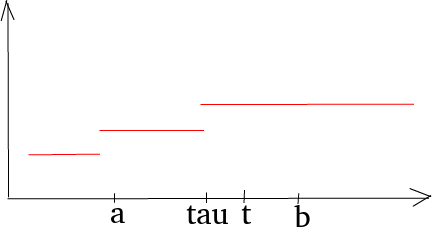
\includegraphics[width=.4\textwidth]{./pictures/3_5.png}
  \caption{График пуассоновского процесса}
  \label{fig:35}
\end{figure}

У пуассоновского процесса есть однородность приращений
\begin{gather*}
  P \left\{
    N \left( t \right) - N \left( a \right) = 1 \; \middle| \;
    N \left( b \right) - N \left( a \right) = 1 \right\} =
  P \left\{ N \left( t - a \right) = 1 \; \middle| \; N \left( b - a \right) = 1 \right\} = \\
  = P \left\{ Bin \left( 1, \frac{t - a}{b - a} \right) = 1 \right\} =
\end{gather*}
Это бернуллиевская величина
$$= \frac{t - a}{b - a}.$$
Получилось равномерное распределение, что и требовалось доказать.

\subsubsection*{3.6}

\textit{Задание.}
Пусть $ \left\{ \tau_k \right\}_{k \geq 1}$ --- последовательность независимых показательно
распределённых случаных величин с параметром $ \lambda $.
Положим
$$T_0 = 0, \,
  T_n = \sum \limits_{k = 1}^n \tau_k, \,
  n \geq 1; \,
  \nu \left( t \right) = \max \left( n \, : \, T_n \leq t \right), \,
  t \geq 0.$$
\begin{enumerate}[label=\alph*)]
  \item Докажите, что
  $$ \lim \limits_{n \to \infty } \frac{T_n}{n} =
    \frac{1}{ \lambda }$$
  почти наверное.
  \item Докажите, что случайная величина $ \tau_1 = T_{ \nu \left( t \right) + 1} - t$
  имеет показательное распределение с параметром $ \lambda $.
  \item Докажите, что $ \left\{ \nu \left( t \right), \, t \geq 0 \right\} $
  является процессом Пуассона с интенсивностью $ \lambda $.
\end{enumerate}

\textit{Решение.}
$\nu \left( t \right) = \max \left( n \, : \, T_n \leq t \right) $ --- случайный процесс.

Посмотрим, как этот процесс выглядит (рис. \ref{fig:36}).

$T_n$ --- это накопительные суммы.

В момент $T_1$ только $T_1 \leq t$, то есть от $T_1$ до $T_2$ значение процесса будет равно единице.

\begin{figure}[h!]
  \centering
  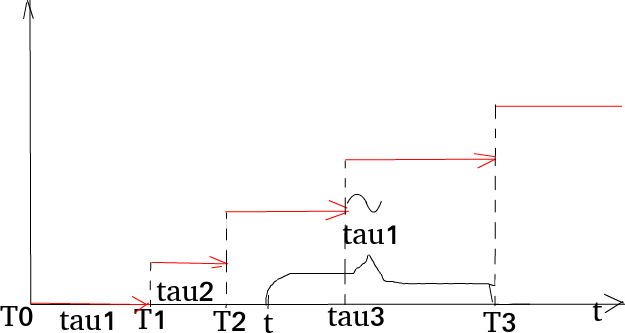
\includegraphics[width=.4\textwidth]{./pictures/3_6.png}
  \caption{График процесса}
  \label{fig:36}
\end{figure}

Тут расставили стрелочки, то ест $ \nu $ --- это непрерывная справа функция.
То есть $ \nu $ --- это модификация пуассоновского процесса.
Конечномерные распределения несут ещё не всю информацию.

\begin{enumerate}[label=\alph*)]
  \item Нужно доказать, что
  $$ \lim \limits_{n \to \infty } \frac{T_n}{n} =
    \frac{1}{ \lambda }$$
  почти наверное.

  Это равенство --- это просто закон больших чисел, потому что
  $$ \frac{1}{n} \sum \limits_{k = 1}^n \tau_k = T_n \to
    M \tau_1 = \frac{1}{ \lambda }.$$

  Сумма $T_n$ сходится к бесконечности.
  Это нужно для того, чтобы определить процесс на всей оси.
  То есть вывод из пункта a) следующий
  $$T_n =
    n \cdot \frac{T_n}{n} \to
    \infty \cdot \frac{1}{ \lambda } =
    \infty $$
  и $ \nu \left( t \right) $ определено при всех $t$.
  \item $ \tilde{ \tau_1}$ --- это величина до следующего прыжка.

  Этот пункт означает, что процесс $ \nu $ имеет однородные приращения.

  Докажем, чо $ \tilde{ \tau_1}$ имеет действительно показательное распределение.
  Проще всего для показательного распределения посчитать
  $$P \left( \tilde{ \tau_1} \right) =
    1 - F =
    1 - \left( 1 - e^{-\lambda s} \right) =
    e^{-\lambda s},$$
  где $F$ --- функция распределения.
  Вопрос: есть ли такое равенство.

  Значит,
  $P \left( \tilde{ \tau_1} > s \right) =
    P \left( T_{ \nu \left( t \right) + 1} > t + s \right) $.
  Величина $T$ берётся в случайный момент.
  Такая вероятность может быть записана через сумму по всем возможным $T$, то есть
  $$P \left( T_{ \nu \left( t \right) + 1} > t + s \right) =
    \sum \limits_{n = 0}^{ \infty }
      P \left( T_n \leq t < T_{n + 1}, \, T_{n + 1} > t + s \right) =$$
  Одно условие убирается
  $$ = \sum \limits_{k = 0}^{ \infty } P \left( T_n \leq t, T_{n + 1} \leq t + s \right) =$$
  Момент $T_{n + 1}$ --- это момент следующего скачка после $T_n$.
  Тогда
  \begin{gather*}
    = \sum \limits_{n = 0}^{ \infty }
      P \left( T_n \leq t, \, T_n + \tau_{n + 1} > t + s \right) = \\
    = \sum \limits_{n = 0}^{ \infty }
      P \left\{ T_n \leq t, \tau_{n + 1} \geq \left( t - T_n \right) + s \right\} =
  \end{gather*}
  Моменты $ \tau_{n + 1}$ и $T_n$ --- независимые величины.
  $$= \sum \limits_{n = 0}^{ \infty }
    MP \left[ T_n \leq t, \, \tau_{n + 1} > \left( t - T_n \right) + s \; \middle| \;
    T_n \right] =$$
  Вспомним, какая вероятность $P \left( \tau > x \right) = e^{-\lambda x}$.
  Тогда
  $$P \left( \tau > x + y \right) =
    e^{-\lambda \left( x + y \right) } =
    e^{-\lambda x} e^{-\lambda y}.$$
  Для показательных величин выполнено соотношение
  $$P \left( \tau > x + y \right) =
    e^{-\lambda y} P \left( \tau > x \right) $$
  --- свойство отсутствия последействия.
  $$= \sum \limits_{n = 0}^{ \infty }
      e^{-\lambda s} P \left( T_n \leq t, \tau_{n + 1} > t - T_n \right) =
    e^{-\lambda s} \sum \limits_{n = 0}^{ \infty } P \left( T_n \leq t < T_{n + 1} \right) =$$
  Такая сумма равна единице,
  потому что $t$ всегда попадает между $T_n$ и $T_{n + 1}$ при каком-то $n$, потому
  $$= e^{-\lambda s},$$
  так что такая величина $ \tilde{ \tau_1}$ действительно имеет показательное распределение.
  \item Найдём конечномерные распределения $ \nu \left( t \right) $.
  Имеем
  \begin{gather*}
    P \left\{
      \nu \left( t_1 \right) = k_1, \nu \left( t_2 \right) = k_2, \dotsc,
      \nu \left( t_n \right) = k_n
    \right\} = \\
    = P \left(
      \sum \limits_{l = 1}^{k_1} \tau_l \leq t_1 < \sum \limits_{l = 1}^{k_1 + 1} \tau_l, \dotsc,
      \sum \limits_{l = 1}^{k_n} \tau_l \leq t_n < \sum \limits_{l = 1}^{k_n + 1} \tau_l
    \right) = \\
    = \idotsint \limits_{k_n + 1}
      \lambda^{k_n + 1} e^{-\lambda \left( x_{k_1} + \dotsc + x_{k_n} + 1 \right) }
    dx_{k_n + 1} \dotsc dx_1 = \\
    = \lambda^{k_n + 1} \cdot
    \idotsint \limits_{k_n, \, 0 < x_{k_1} + \dotsc + x_{k_n} \leq t, \, t = \sum t_i}
      e^{-\lambda \left( x_{k_1} + \dotsc + x_{k_n} \right) } \times \\
       \times \int \limits_{t - \sum \limits_{i = 1}^{k_n} x_i}
        e^{-\lambda x_{k_n + 1}} dx_{k_n + 1} \dotsc dx_1 =
  \end{gather*}
  Возьмём последний интеграл
  $$ \int \limits_{t - \sum \limits_{i = 1}^{k_n} x_i} e^{-\lambda x_{k_n + 1}} dx_{k_n + 1} =
    \left.
      -\frac{1}{ \lambda } \cdot e^{-\lambda x_{k_n + 1}}
    \right|_{t - \sum \limits_{i = 1}^{k_n} x_i}^{+ \infty }.$$
  Подставляем и получаем
  \begin{gather*}
    = \frac{ \lambda^{k_n + 1}}{ \lambda }
    \idotsint \limits_{k_n, \, 0 < x_{k_1} + \dotsc + x_{k_n} \leq t}
      e^{-\lambda \sum \limits_{i = k_1}^{k_n} x_i}
      e^{-\lambda t + \lambda \sum \limits_{i = k_1}^{k_n} x_i} dx_{k_n} \dotsc dx_{k_1} = \\
   = \lambda^{k_n} e^{-\lambda t}
   \idotsint \limits_{0 < \sum \limits_{i = k_1}^{k_n} x_i \leq 1} dx_{k_n} \dotsc dx_{k_1} =
 \end{gather*}
  Чтобы понять, чему будет равен этот интеграл, рассмотрим частные случаи:
  \begin{enumerate}
    \item когда есть двойной интеграл
    \begin{gather*}
      \iint \limits_{0 < x_1 + x_2 \leq t} dx_2 dx_1 =
      \int \limits_0^t \int \limits_0^{t - x_1} dx_2 dx_1 =
      \int \limits_0^t \left. x_2 \right|_0^{t - x_1} dx_1 = \\
       =\int \limits_0^t \left( t - x_1 \right) dx_1 =
      t \int \limits_0^t dx_1 - \int \limits_0^t x_1 dx_1 =
      t^2 - \left. \frac{x^2}{2} \right|_0^t =
      t^2 - \frac{t^2}{2} = \\
      = \frac{t^2}{2} =
      \frac{t^2}{2!};
    \end{gather*}
    \item когда есть тройной интеграл
    \begin{gather*}\iiint \limits_{0 < x_1 + x_2 + x_3 \leq t} dx_3 dx_2 dx_1 =
      \int \limits_0^t \int \limits_0^{t - x_1} \int \limits_0^{t - x_1 - x_2} dx_3 dx_2 dx_1 = \\
      = \int \limits_0^t \int \limits_0^{t - x_1} \left( t - x_1 - x_2 \right) dx_2 dx_1 = \\
      = \int \limits_0^t \left(
        t \int \limits_0^{t - x_1} dx_2 - x_1 \int \limits_0^{t - x_1} dx_2 -
        \int \limits_0^{t - x_1} x_2 dx_2 \right) dx_1 = \\
      = \int \limits_0^t \left[
        t \left( t - x_1 \right) - x_1 \left( t - x_1 \right) - \frac{ \left( t - x_1 \right)^2}{2}
      \right] dx_1 = \\
      = \int \limits_0^t
        \frac{2t^2 - 2tx_1 - 2tx_1 + 2x_1^2 - t^2 + 2tx_1 - x_1^2}{2} dx_1 \times \\
      \times \int \limits_0^t \frac{t^2 - 2x_1 t + x_1^2}{2} dx_1 =
      \int \limits_0^t \frac{ \left( t - x_1 \right)^2}{2} dx_1 =
      \left. -\frac{1}{2} \cdot \frac{ \left( t - x_1 \right)^3}{3} \right|_0^t = \\
      = \frac{t^3}{2 \cdot 3} =
      \frac{t^3}{3!}.
    \end{gather*}
  \end{enumerate}
  Значит,
  $$ \idotsint \limits_{0 < \sum \limits_{i = k_1}^{k_n} x_i \leq 1} dx_{k_n} \dotsc dx_{k_1} =
    \frac{t^{k_n}}{k_n!}.$$

  Тогда вероятность равна
  $$= \frac{ \lambda^{k_n} e^{-\lambda t} t^{k_n}}{k_n!} =
    \frac{ \left( \lambda t \right)^{k_n}}{k_n!} \cdot e^{-\lambda t}.$$
  Получился процесс Пуассона с интенсивностью $ \lambda $.
\end{enumerate}

\subsubsection*{3.7}

\textit{Задание.}
Пусть $N = \left\{ N \left( t \right), \, t \geq 0 \right\} $ ---
процесс Пуассона с параметром $ \lambda $ и пусть $ \left\{ Y_n \right\}_{n \geq 1}$ ---
независимая от $N$ последовательность независимых бернуллиевских случайных величин с парметром
$p \in \left( 0, 1 \right) $.
Положим
$$S_n = Y_1 + \dotsc + Y_n.$$
Докажите, что процесс $ \xi = \left\{ S_{N \left( t \right)}, \, t \geq 0 \right\} $
является процессом Пуассона с параметром $ \lambda t$.

\textit{Решение.}
Пуассоновский процесс
$$N \left( t \right) =
  \sum \limits_{n = 1}^{N \left( t \right) } 1$$
--- число событий до момента $N \left( t \right) $.
В $ \xi $ складываем не 1, а $Y_i = 0$ или $1$.

Начнём с того, что посчитаем одномерные распределения и посмотрим,
что это тоже пуассоновские величины.
Есть сумма случайного числа слагаемых.
Нужно перебирать все возможные значения $N \left( t \right) $.
Имеем
\begin{gather*}
  P \left\{ S_{N \left( t \right) } = k \right\} =
  P \left\{ Y_1 + \dotsc + Y_{N \left( t \right) } = k \right\} = \\
  = \sum \limits_{n = 0}^{ \infty }
    P \left\{ N \left( t \right) = n, \, Y_1 + \dotsc + Y_n = k \right\} =
\end{gather*}
Сумма $Y_1 + \dotsc + Y_n $ --- биномиальная величина
$$= \sum \limits_{n = k}^{ \infty }
    \frac{ \left( \lambda t \right)^n}{n!} \cdot
    e^{-\lambda t} \cdot C_n^k p^k \left( 1 - p \right)^{n - k} =$$
Преобразуем
$$= e^{-\lambda t} p^k \cdot
  \sum \limits_{n = k}^{ \infty }
    \frac{ \left( \lambda t \right)^n}{n!} \cdot C_n^k \left( 1 - p \right)^{n - k} =$$
Распишем $C_n^k$ явно
$$= e^{-\lambda t} p^k \cdot
  \sum \limits_{n = k}^{ \infty }
    \frac{ \left( \lambda t \right)^n}{n!} \cdot
    \frac{n!}{k! \left( n - k \right)!} \cdot \left( 1 - p \right)^{n - k} =
  \frac{e^{-\lambda t} p^k}{k!} \cdot
  \sum \limits_{n = k}^{ \infty }
    \frac{ \left( \lambda t \right)^{n + k} \left( 1 - p \right)^{n - k}}{ \left( n - k \right)!} =$$
Имеем ряд для экспоненты.
Заменим $n - k$ на новый индекс суммирования
$$= \frac{e^{-\lambda t} p^k}{k!} \cdot
  \sum \limits_{n = 0}^{ \infty }
    \frac{ \left( \lambda t \right)^{n + k} \left( 1-  p \right)^n}{n!} =$$
Выносим $ \left( \lambda t \right)^k$ за знак суммы
$$= \frac{e^{-\lambda t} p^k \left( \lambda t \right)^k}{k!} \cdot
  \sum \limits_{n = 0}^{ \infty } \frac{ \left( \lambda t \right)^n \left( 1 - p \right)^n}{n!} =
  \frac{e^{-\lambda t} \left(p \lambda t \right)^k}{k!} \cdot e^{ \lambda t \left( 1 - p \right) } =
  \frac{e^{-\lambda pt} \left( \lambda pt \right)^k}{k!}$$
--- пуассоновская вероятность.

Вывод: $S_{N \left( t \right) } \sim Pois \left( \lambda pt \right) $,
то есть у такого процесса одномерные распределения такие же,
как у пуассоновского с параметром $ \lambda pt$.

\addcontentsline{toc}{section}{Домашнее задание}
\section*{Домашнее задание}

\subsubsection*{3.11}

\textit{Задание.}
Пусть $N = \left\{ N \left( t \right), \, t \geq 0 \right\} $ ---
процесс Пуассона с интенсивностью $ \lambda = 5$.
Вычислите вероятности:
\begin{enumerate}[label=\alph*)]
  \item $P \left( N \left( 2 \right) \geq 3, \, N \left( 5 \right) \leq 4 \right) $;
  \item $P \left(
    N \left( 2 \right) \geq 3, \, N \left( 3 \right) \geq 4, \, N \left( 5 \right) \leq 3 \right) $;
  \item $P \left(
    N \left( 2 \right) = 3, \, N \left( 3 \right) = 5, \, N \left( 4 \right) \leq 6 \right) $;
  \item $P \left( N \left( 2 \right) = 3 \; \middle| \; N \left( 3 \right) = 5 \right) $;
  \item $P \left( N \left( 3 \right) = 5 \; \middle| \; N \left( 2 \right) = 3 \right) $.
\end{enumerate}

\textit{Решение.}
\begin{enumerate}[label=\alph*)]
  \item Рассмотрим все возможные случаи
  \begin{gather*}
    P \left( N \left( 2 \right) \geq 3, \, N \left( 5 \right) \leq 4 \right) = \\
    = P \left\{ N \left( 2 \right) = 3, \, N \left( 5 \right) = 3 \right\} +
    P \left\{ N \left( 2 \right) = 3, \, N \left( 5 \right) = 4 \right\} + \\
    + P \left\{ N \left( 2 \right) = 4, \, N \left( 5 \right) = 4 \right\} =
  \end{gather*}
  Нужно перейти к приращениям, потому что они независимы
  \begin{gather*}
    = P \left\{
      N \left( 2 \right) = 2, \, N \left( 5 \right) - N \left( 2 \right) = 3 - 3 \right\} + \\
    + P \left\{
      N \left( 2 \right) = 3, \, N \left( 5 \right) - N \left( 2 \right) = 4 - 3 \right\} + \\
    + P \left\{
      N \left( 2 \right) = 4, \ ,N \left( 5 \right) - N \left( 2 \right) = 4 - 4 \right\} = \\
    = P \left\{ N \left( 2 \right) = 3 \right\} P \left\{ N \left( 3 \right) = 0 \right\} +
    P \left\{ N \left( 2 \right) = 3 \right\} P \left\{ N \left( 3 \right) = 1 \right\} + \\
    + P \left\{ N \left( 2 \right) = 4 \right\} P \left\{ N \left( 3 \right) = 0 \right\} = \\
    = \frac{10^3}{3!} \cdot e^{-10} \cdot \frac{15^0}{0!} \cdot e^{-15} +
    \frac{10^3}{3!} \cdot e^{-10} \cdot \frac{15^1}{1!} \cdot e^{-15} + \\
    + \frac{10^4}{4!} \cdot e^{-10} \cdot \frac{15^0}{0!} \cdot e^{-15} =
    \frac{10^3}{3!} \cdot e^{-25} + \frac{10^3}{3!} \cdot e^{-25} \cdot 15 +
    \frac{10^4}{4!} \cdot e^{-25} = \\
    = \frac{10^3}{3!} \cdot e^{-25} \cdot 16 + \frac{10^4}{4!} \cdot e^{-25};
  \end{gather*}
  \item с ростом времени значение процесса Пуассона не должно уменьшаться
  $P \left(
    N \left( 2 \right) \geq 3, \, N \left( 3 \right) \geq 4, \, N \left( 5 \right) \leq 3 \right) =
    0$;
  \item как в первом пункте рассмотрим все возможные случаи
  \begin{gather*}
    P \left(
    N \left( 2 \right) = 3, \, N \left( 3 \right) = 5, \, N \left( 4 \right) \leq 6 \right) = \\
    = P \left\{
      N \left( 2 \right) = 3, \, N \left( 3 \right) = 5, \, N \left( 4 \right) = 5 \right\} + \\
    + P \left\{
      N \left( 2 \right) = 3, \, N \left( 3 \right) = 5, \, N \left( 4 \right) = 6 \right\} =
  \end{gather*}
  Нужно перейти к приращениям, потому что они независимы
  \begin{gather*}
    = P \left\{
      N \left( 2 \right) = 3, \, N \left( 3 \right) - N \left( 2 \right) = 5 - 3, \,
      N \left( 4 \right) - N \left( 3 \right) = 5 - 5 \right\} + \\
    + P \left\{
      N \left( 2 \right) = 3, \, N \left( 3 \right) - N \left( 2 \right) = 5 - 3, \,
      N \left( 4 \right) - N \left( 3 \right) = 6 - 5 \right\} = \\
    = P \left\{ N \left( 2 \right) = 3 \right\} \cdot P \left\{ N \left( 1 \right) = 2 \right\} \cdot
    P \left\{ N \left( 1 \right) = 0 \right\} + \\
    + P \left\{ N \left( 2 \right) = 3 \right\} \cdot P \left\{ N \left( 1 \right) = 2 \right\} \cdot
    P \left\{ N \left( 1 \right) = 1 \right\} = \\
    = \frac{10^3}{3!} \cdot e^{-10} \cdot \frac{5^2}{2!} \cdot e^{-5} \cdot \frac{5^0}{0!} \cdot
    e^{-5} +
    \frac{10^3}{3!} \cdot e^{-10} \cdot \frac{5^2}{2!} \cdot e^{-5} \cdot \frac{5^1}{1!} \cdot
    e^{-5} = \\
    = \frac{10^3}{3!} \cdot e^{-20} \cdot \frac{5^2}{2!} +
    \frac{10^3}{3!} \cdot e^{-20} \cdot \frac{5^3}{2!} =
    \frac{10^3}{3!} \cdot e^{-20} \cdot \frac{5^2}{2!} \cdot 6 =
    10^{-20} \cdot 12500;
  \end{gather*}
  \item по определению условной вероятности
  $$P \left( N \left( 2 \right) = 3 \; \middle| \; N \left( 3 \right) = 5 \right) =
    \frac{P \left\{ N \left( 2 \right) = 3, \, N \left( 3 \right) = 5 \right\} }{P \left\{ N \left( 3 \right) = 5 \right\} } =$$
  Перейдём к приращениям и подставим выражения для вероятностей
  $$= \frac{ \frac{10^3}{3!} \cdot e^{-10} \cdot \frac{5^2}{2!} \cdot e^{-5}}{ \frac{15^5}{5!} \cdot e^{-15}} =$$
  Экспоненты сокращаются
  $$= \frac{10^3 \cdot 5^2 \cdot 5!}{3! \cdot 2! \cdot 15^5} =
  \frac{80}{243};$$
  \item аналогично предыдущему пункту
  $$P \left( N \left( 3 \right) = 5 \; \middle| \; N \left( 2 \right) = 3 \right) =
    \frac{P \left\{ N \left( 3 \right) = 5, \, N \left( 2 \right) = 3 \right\} }{P \left\{ N \left( 2 \right) = 3 \right\} } =$$
  Перейдём к приращениям
  $$= \frac{P \left\{ N \left( 2 \right) = 3 \right\} P \left\{ N \left( 1 \right) = 2 \right\} }{P \left\{ N \left( 2 \right) = 3 \right\} } =
    P \left\{ N \left( 1 \right) = 2 \right\} =
    \frac{5^2}{2!} \cdot e^{-5}.$$
\end{enumerate}

\subsubsection*{3.12}

\textit{Задание.}
Пусть $N = \left\{ N \left( t \right), \, t \geq 0 \right\} $ ---
процесс Пуассона с интенсивностью $ \lambda = 1$.
Найдите характеристическую функцию случайной величины
$$N \left( 3 \right) - N \left( 2 \right) + N \left( 1 \right).$$

\textit{Решение.}
$N \left( t \right) \sim Pois \left( t \right) $.
Процесс Пуассона имеет однородность приращений
$N \left( 3 \right) - N \left( 2 \right) \sim
  N \left( 3 - 2 \right) =
  N \left( 1 \right)
  \sim Pois \left( 1 \right) $,
а $N \left( 1 \right) \sim Pois \left( 1 \right) $.

Приращения $N \left( 3 \right) - N \left( 2 \right) $ и $N \left( 1 \right) $ --- независимы,
следовательно,
$$N \left( 3 \right) - N \left( 2 \right) + N \left( 1 \right) \sim
  Pois \left( 1 + 1 \right) =
  Pois \left( 2 \right).$$

Тогда характеристическая функция
$ \varphi_{N \left( 3 \right) - N \left( 2 \right) + N \left( 1 \right) } \left( t \right) =
  e^{2 \left( e^{it} - 1 \right) }$.

\subsubsection*{3.13}

\textit{Задание.}
Пусть $N = \left\{ N \left( t \right), \, t \geq 0 \right\} $ ---
процесс Пуассона с интенсивностью $ \lambda $.
Найдите условную вероятность
$P \left( N \left( s \right) = k \; \middle| \; N \left( t \right) = n \right) $ при $s > t$
и вычислите условное математическое ожидание
$M \left[ N \left( s \right) \; \middle| \; N \left( t \right) \right] $ для $s >  t$.

\textit{Решение.}
$N \left( t \right) \sim Pois \left( \lambda t \right) $.

Что такое условное математическое ожидание?

$N \left( s \right) $ и $N \left( t \right) $ --- дискретные величины, то есть
$$M \left[ N \left( s \right) \; \middle| \; N \left( t \right) \right] =
  \sum \limits_{k = 0}^{ \infty }
    k \cdot P \left\{ N \left( s \right) = k \; \middle| \; N \left( t \right) = n \right\}.$$

Отдельно посчитаем условную вероятность, а потом по ней возьмём математическое ожидание
$$P \left\{ N \left( s \right) = k \; \middle| \; N \left( t \right) = n \right\} =
  \frac{P \left\{ N \left( s \right) = k, \, N \left( t \right) = n \right\} }{P \left\{ N \left( t \right) = n \right\} } =$$
Перепишем через приращения и воспользуемся их независимостью
$$= \frac{P \left( N \left( t \right) = n \right\} P \left\{ N \left( s - t \right) = k - n \right\} }{P \left\{ N \left( t \right) = n \right\} } =$$
Сократим одинаковые множители в числителе и знаменателе
$$= P \left\{ N \left( s - t \right) = k - n \right\} =$$
Подставим пуассоновские вероятности
$$= \frac{ \left[ \lambda \left( s - t \right) \right]^{k - n}}{ \left( k - n \right)!} \cdot
  e^{-\lambda \left( s - t \right) }.$$

Имеем пуассоновское распределение с параметром $ \lambda \left( s - t \right) $.

Вывод: при условии $N \left( t \right) = n$ мы нашли распределение
$$N \left( s \right) \sim Pois \left( \lambda \left( s - t \right) \right).$$

Условное математическое ожидание
$$M \left[ N \left( s \right) \; \middle| \; N \left( t \right) \right] =
  MPois \left( \lambda \left( s - t \right) \right) =
  \lambda \left( s - t \right).$$

\subsubsection*{3.14}
\textit{Задание.}
Пусть
$ \xi = \left\{ \xi \left( t \right), \, t \geq 0 \right\}, \,
  \eta = \left\{ \eta \left( t \right), \, t \geq 0 \right\} $
являются независимыми процессами Пуассона с параметрами $ \lambda $ и $ \mu $ соответственно.
Положим $ \zeta \left( t \right) = \xi \left( t \right) + \eta \left( t \right) $.
Докажите, что процесс $ \zeta = \left\{ \zeta \left( t \right), \, t \geq 0 \right\} $
является процессом Пуассона с параметром $ \lambda + \mu $.

\textit{Решение.}
$$ \varphi_{ \zeta } \left( t \right) =
  \varphi_{ \xi + \eta } \left( t \right) =
  \varphi_{ \xi } \left( t \right) \varphi_{ \eta } \left( t \right) =
  e^{ \lambda t \left( e^{it} - 1 \right) } e^{ \mu t \left( e^{it} - 1 \right) } =
  e^{ \left( \lambda + \mu \right) t \left( e^{it} - 1 \right) }.$$
Следовательно, $ \zeta \sim Pois \left( \lambda + \mu \right) $.

\subsubsection*{3.15}

\textit{Задание.}
Пусть $ \left\{ N \left( t \right), \, t \geq 0 \right\} $ ---
процесс Пуассона с интенсивностью $ \lambda $.
Выясните, какой из следующих процессов является пуассоновским:
\begin{gather*}
  \left\{ N_1 \left( t \right) = 2N \left( t \right), \, t \geq 0 \right\};
  \left\{ N_2 \left( t \right) = N \left( 2t \right), \, t \geq 0 \right\};
  \left\{ N_3 \left( t \right) = N \left( t^2 \right), \, t \geq 0 \right\}; \\
  \left\{ N_4 \left( t \right) = N \left( t + s \right) - N \left( s \right), \, t \geq 0 \right\},
\end{gather*}
где $s > 0$ --- фиксированное число.
Для пуассоновских процессов укажите их интенсивность.

\textit{Решение.}
$$P \left\{ N_1 \left( t \right) = k \right\} =
  P \left\{ 2N \left( t \right) = k \right\} =
  P \left\{ N \left( t \right) = \frac{k}{2} \right\} =
  0,$$
так как пуассоновский процесс принимает только неотрицательные целые значения.
Следовательно, $ \left\{ N_1 \left( t \right), \, t \geq 0 \right\} $ --- не процесс Пуассона.

$$P \left\{ N_2 \left( t \right) = k \right\} =
  P \left\{ N \left( 2t \right) = k \right\} =
  \frac{ \left( \lambda \cdot 2t \right)^k}{k!} \cdot e^{-2 \lambda t}$$
--- процесс Пуассона с интенсивностью $2 \lambda $.
Независимость и однородность приращений выполняются.


Перейдём к третьему процессу
$$P \left\{ N_3 \left( t \right) = k \right\} =
  P \left\{ N \left( t^2 \right) = k \right\} =
  \frac{ \left( \lambda t^2 \right)^k}{k!} \cdot e^{-\lambda t^2} \sim
  Pois \left( \lambda t^2 \right) \not \sim
  Pois \left( \mu t \right),$$
значит, процесс не пуассоновский.

$$P \left\{ N_4 \left( t \right) = k \right\} =
  P \left\{ N \left( t + s \right) - N \left( s \right) = k \right\} =
  P \left\{ N \left( t \right) = k \right\} =
  \frac{ \left( \lambda t \right)^k}{k!} \cdot e^{-\lambda t}$$
--- процесс Пуассона с интенсивностью $ \lambda $.

\subsubsection*{3.16}

\textit{Задание.}
Пусть $N = \left\{ N \left( t \right), \, t \geq 0 \right\} $ ---
процесс Пуассона с интенсивностью $ \lambda $ и пусть $ \xi_1, \xi_2, \dotsc $ ---
независимые от процесса $N$
независимые одинаково распределённые случайные величины с математическим ожиданием $m$.
Пусть
$$X \left( t \right) =
  \sum \limits_{i = 1}^{N \left( t \right) } \xi_i.$$
Докажите, что $M \left[ X \left( t \right) \right] = m \lambda t$.

\textit{Решение.}
$N \left( t \right) \sim Pois \left( \lambda t \right) $.

Вычислим математическое ожидание
$$MX \left( t \right) =
  M \left( \sum \limits_{i = 1}^{N \left( t \right) } \xi_i \right) =
  M \sum \limits_{i = 1}^{ \infty }
    \left( \mathbbm{1} \left\{ N \left( t \right) = i \right\} \xi_i \right) =$$
Математическое ожидание индикатора --- вероятность
$$= m \sum \limits_{i = 1}^{ \infty } i \cdot P \left\{ N \left( t \right) = i \right\} =
  mMN \left( t \right) =
  m \lambda t.$$

\subsubsection*{3.17}

\textit{Задание.}
Пусть $ \left\{ N \left( t \right), \, t \geq 0 \right\} $ ---
процесс Пуассона с интенсивностью $ \lambda $.
Используя пункт а) задачи 3.6 докажите, что
$$ \lim \limits_{t \to \infty } \frac{N \left( t \right) }{t} = \lambda \, a.s.$$

\textit{Решение.}
Надо проверить, что для пуассоновского процесса
$$ \lim \limits_{t \to \infty } \frac{N \left( t \right) }{t} = \lambda \, a.s.$$

В задаче 3.6 доказали, что
$$ \frac{T_n}{n} \to
  \frac{1}{ \lambda }$$
с помощью закона больших чисел.

$N \left( T_n \right) = n$ --- значение $T_n$-го скачка (рис. \ref{fig:317}).

$$ \frac{T_n}{n} \to \frac{1}{ \lambda } \leftrightarrow
  \frac{T_n}{N \left( T_n \right) } \to \frac{1}{ \lambda }.$$
Тогда
$$ \frac{N \left( T_n \right) }{T_n} \to \lambda.$$

Из такой сходимости следует сходимость по всем моментам времени.
Нужно вывести, что
$$ \frac{N \left( t \right) }{t} \to \lambda.$$

\begin{figure}[h!]
  \centering
  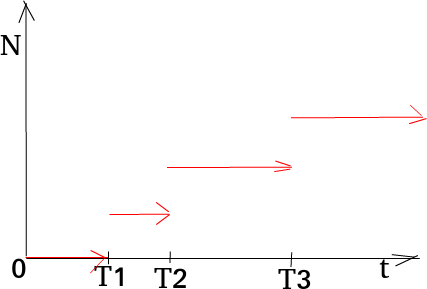
\includegraphics[width=.4\textwidth]{./pictures/3_17.png}
  \caption{График пуассоновского процесса}
  \label{fig:317}
\end{figure}

\subsubsection*{3.18}

\textit{Задание.}
Прибытие посетителей в магазин является процессом Пуассона с интенсивностью $ \lambda = 20$
посетителей в час.
Вычислите среднее количество продаж на протяжении одного восьмичасового рабочего дня,
если вероятность того, что посетитель магазина сделает покупку равна $0.3$.

\textit{Решение.}
$N \left( t \right) $ --- количество покупок за время $ \left[ 0, t \right] $.

Обозначим количество покупок как
$$n \left( t \right) =
  \sum \limits_{k = 1}^{N \left( t \right) } y_k,$$
где $y_k = \mathbbm{1}$\{$k$-й посетитель магазина сделает покупку\}.

При этом $P \left\{ y_k = 1 \right\} = 0.3$, а $P \left\{ y_k = 0 \right\} = 1 - 0.3 = 0.7$.

То есть $y_k$ имеет распределение Бернулли.

Из задачи 3.7 получает, что $n \left( t \right) \sim Pois \left( 0.3 \lambda \right) $.

Среднее количество покупок за 8 часов
$Mn \left( 8 \right) =
  8 \cdot 0.3 \lambda =
  8 \cdot 0.3 \cdot 20 =
  48$.

\subsubsection*{3.19}

\textit{Задание.}
Большой супермаркет имеет три входа.
Прибытие посетителей через каждые двери образуют процессы Пуассона с интенсивностями
$ \lambda_1 = 110, \, \lambda_2 = 90, \, \lambda_3 = 160$ посетителей в час.
30\% посетителей составляют мужчины.
Вероятность того, что посетитель-мужчина сделает покурку, равна $0.8$, а вероятность того,
что женщина-посетитель сделает покупку, равна $0.1$.
Средняя цена покупки составляет 100 грн.
\begin{enumerate}[label=\alph*)]
  \item Вычислите среднюю выручку супермаркета за 10-часовой рабочий день.
  \item Вычислите вероятность того, что третья женщина-посетитель, которая сделает покупку,
  прибудет в магазин в первые 15 минут.
  Вычислите среднее время её прибытия в магазин.
\end{enumerate}

\textit{Решение.}
\begin{enumerate}[label=\alph*)]
  \item $t = 10$.

  Найдём общую интенсивность $ \lambda = 110 + 90 + 160 = 360$ посетителей в час.

  Найдём $ \lambda_m = 360 \cdot 0.3 = 108$ посетителей-мужчин в час и
  $$ \lambda_w =
    360 \cdot 0.7 =
    252$$
  посетителей-женщин в час.

  Пусть $n \left( t \right) $ --- число покупок в день.
  Тогда
  $$Mn \left( t = 10 \right) =
    M \left[ n_m \left( 10 \right) + n_w \left( 10 \right) \right] =
    10 \cdot 108 \cdot 0.8 + 10 \cdot 252 \cdot 0.1 =
    1116.$$

  Следовательно, средняя выручка равна
  $$100Mn \left( t = 10 \right) =
    100 \cdot 1116 =
    111600.$$
  \item Пусть $ \lambda_w'$ --- интенсивность покупок, сделанных женщинами.

  $ \lambda_w' = \lambda_w \cdot 0.1 = 25.2$ покупки в час.

  Пусть $N \left( t \right) \sim Pois \left( \lambda_w' t \right) $ ---
  количество женщин-посетителей, прибывших в магазин до момента времени $t$.

  Тогда
  \begin{gather*}
    P \left\{ N \left( 15 minutes \right) = 3 \right\} =
    P \left\{ N \left( \frac{1}{4} \right) = 3 \right\} =
    e^{-25.2 \cdot \frac{1}{4}} \cdot \frac{ \left( -\frac{1}{4} \cdot 25.2 \right)^3}{3!} = \\
    = e^{-6.3} \cdot \frac{250}{6} =
    0.0019 \cdot 41.6 =
    0.08.
  \end{gather*}

  Тогда среднее время её прибытия в магазин
  $$M \tau =
    \frac{3}{ \lambda_w'} =
    \frac{3}{25.2} =
    0.12$$
  часов.
\end{enumerate}

\addcontentsline{toc}{chapter}{Занятие 4. Гауссовские процессы}
\chapter*{Занятие 4. Гауссовские процессы}

\addcontentsline{toc}{section}{Контрольные вопросы и задания}
\section*{Контрольные вопросы и задания}

\subsubsection*{Приведите определение гауссовского процесса.}

Процесс $ \left\{ X \left( t \right), \, t \in T \right\} $ --- гауссовский, если
$$ \sum \limits_{k = 1}^n \lambda_k X \left( t_k \right) $$
--- гауссовская случайная величина $ \forall \vec{ \lambda } \in \mathbb{R}^n$ и
$ \forall t_1, \dotsc, t_n \in T$.

Эквивалентно: $ \left( X \left( t_1 \right), \dotsc, X \left( t_n \right) \right)^T$ ---
гауссовский вектор.

\subsubsection*{Запишите плотность конечномерных распределений гауссовского процесса.}

$$p =
  \frac{1}{ \left( \sqrt{2 \pi} \right)^n} \cdot \frac{1}{ \sqrt{det \, A}} \cdot
  e^{-\frac{1}{2} \left[ A^{-1} \left( \vec{x} - \vec{a} \right), \vec{x} - \vec{a} \right] },$$
если $det \, A > 0$.
Квадратные скобки в степени экспоненты --- это скалярное произведение,
или квадратичная форма матрицы, обратной к ковариации.

\subsubsection*{Приведите определение и сформулируйте основные свойства ковариационной функции.}

$K \left( t, s \right) =
  cov \left[ X \left( t \right), X \left( s \right) \right] $.

Гауссовский процесс существует, из теомеры Колмогорова, с функциями $m$ и $K$ тогда и только тогда,
когда функция $K \left( s, t \right) = K \left( t, s \right) $ --- симметричная, и $K$ ---
неотрицательно определённая, то есть
$$ \sum \limits_{k, j = 1}^n c_k c_j K \left( t_k, t_j \right) \geq
  0.$$

Тут неравенство возможно для любых $c_1, \dotsc, c_n, t_1, \dotsc, t_n$.

\subsubsection*{4.2}

\textit{Задание.}
Выясните, существует ли случайный процесс с ковариационной функцией
\begin{enumerate}[label=\alph*)]
  \item $K \left( t, s \right) = \min \left( t, s \right) $;
  \item $K \left( t, s \right) =
    \left( 1 - \left| t - s \right| \right) \cdot
    \mathbbm{1} \left\{ \left| t - s \right| < 1 \right\}; \,
    t, s \in \mathbb{R}$.
\end{enumerate}

\textit{Решение.}
\begin{enumerate}[label=\alph*)]
  \item $K \left( t, s \right) = \min \left( t, s \right) $.

  Такой процесс есть.
  Какой?
  Винеровский;
  \item $K \left( t, s \right) =
    \left( 1 - \left| t - s \right| \right) \cdot
    \mathbbm{1} \left\{ \left| t - s \right| < 1 \right\}; \,
    t, s \in \mathbb{R}$.

  Если такой процесс есть, то мы его не встречали раньше.
  Симметричность очевидна.
  Вопрос: будет ли такая функция неотрицательно определена?

  Функция зависит только от разности.
  Сейчас $K \left( t, s \right) = \varphi \left( t - s \right) $, где
  $$ \varphi \left( t \right) =
    \begin{cases}
      1 - \left| t \right| , \qquad \left| t \right| \leq 1, \\
      0, \qquad \left| t \right| > 1.
    \end{cases}$$
  Так что
  $$ \sum \limits_{k, j = 1}^n c_k c_j K \left( t_k, t_j \right) =
    \sum \limits_{k, j = 1}^n c_k c_j \varphi \left( t_k - t_j \right) \geq
    0$$
  --- это условие неотрицательной определённости для характеристической функции.
  Будет ли эта функция $ \varphi $ характеристической?
  То есть вопрос в задаче равносилен следующему: будет ли
  $$ \varphi \left( t \right) =
    \begin{cases}
      1 - \left| t \right| , \qquad \left| t \right| \leq 1, \\
      0, \qquad \left| t \right| > 1.
    \end{cases}$$
  характеристической функцией?
  Эта функция изображена на рисунке \ref{fig:42}.

  \begin{figure}[h!]
    \centering
    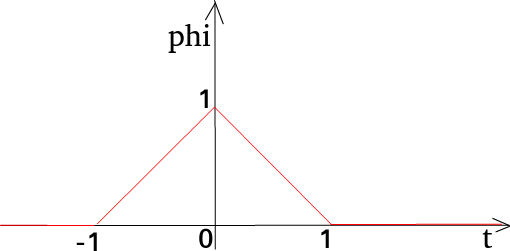
\includegraphics[width=.4\textwidth]{./pictures/4_2.png}
    \caption{График функции $ \varphi \left( t \right) $}
    \label{fig:42}
  \end{figure}


  Она непрерывная, симметричная, в нуле --- единица.
  Если бы это была характеристическая функция
  $$ \varphi \left( t \right) =
    \int \limits_{-\infty }^{+\infty } e^{itx} p \left( x \right) dx$$
  --- преобразование Фурье плотности $p \left( x \right) $.
  Плотность можно найти через обратное преобразование Фурье
  $$p \left( x \right) =
    \frac{1}{2 \pi } \int \limits_{-\infty}^{+\infty } e^{-itx} \varphi \left( t \right) dt =
    \frac{1}{2 \pi } \int \limits_{-1}^1 e^{-itx} \left( 1 - \left| t \right| \right) dt =$$
  Раскроем модуль
  $$= \frac{1}{2 \pi } \left(
    \int \limits_{-1}^1 e^{-itx} dt + \int \limits_{-1}^0 e^{-itx} tdt -
    \int \limits_0^1 e^{-itx} tdt \right) =$$
  Берём первый интеграл
  $$= \frac{1}{2 \pi } \left(
    \left. -\frac{e^{-itx}}{ix} \right|_{-1}^1 - \int \limits_0^1 e^{itx} tdt -
    \int \limits_0^1 e^{-itx} tdt \right) =$$
  Подставляем пределы интегрирования
  $$= \frac{1}{2 \pi } \left[
    -\frac{e^{-ix}}{ix} + \frac{e^{ix}}{ix} -
    \int \limits_0^1 \left( e^{-itx} + e^{itx} \right) tdt \right] =$$
  Из формулы Эйлера следует, что $e^{-itx} + e^{itx} = 2 \cos \left( tx \right) $.
  Тогда
  $$= \frac{1}{2 \pi }
    \left[ \frac{-e^{-ix} + e^{ix}}{ix} - 2 \int \limits_0^1 \cos \left( tx \right) tdt \right] =$$
  Интегрируем по частям, то есть
  $$u = t, \,
    du = dt, \,
    dv = \cos \left( tx \right) dt, \,
    c = \int \cos \left( tx \right) dt = \frac{1}{x} \cdot \sin \left( xt \right).$$
  Получаем
  $$= \frac{1}{2 \pi } \left[
      \frac{-e^{-ix} + e^{ix}}{ix} -
      2 \cdot \left. \frac{t}{x} \cdot \sin \left( xt \right) \right|_0^1 +
      2 \int \limits_0^1 \frac{1}{x} \cdot \sin \left( xt \right) dt \right] =$$
  Подставляем пределы интегрирования и берём интеграл от синуса
  $$= \frac{1}{2 \pi } \left[
    \frac{-e^{-ix} + e^{ix}}{ix} - \frac{2}{x} \cdot \sin x -
    \left. \frac{2}{x^2} \cdot \cos \left( xt \right) \right|_0^1 \right] =$$
  Снова подставляем пределы интегрирования
  $$= \frac{1}{2 \pi } \left(
    \frac{-e^{-ix} + e^{ix}}{ix} - \frac{2}{x} \cdot \sin x - \frac{2}{x^2} \cdot \cos x +
    \frac{2}{x^2} \right) =$$
  Из формулы Эйлера следует, что $e^{ix} - e^{-ix} = 2i \sin x$.
  Тогда
  $$= \frac{1}{2 \pi} \left[
    \frac{2 \sin x}{x} - \frac{2 \sin x}{x} + \frac{2}{x^2} \left( -\cos x + 1 \right) \right] =
  \frac{1}{ \pi x^2} \left( 1 - \cos x \right).$$

  Нашли обратное преобразование Фурье
  $$ \varphi \left( t \right) =
    \int \limits_{-\infty }^{+\infty } e^{itx} p \left( x \right) dx $$
  и $p \left( x \right) \geq 0$.

  Должно выполняться условие нормировки
  $$ \int \limits_{-\infty }^{+\infty } p \left( x \right) dx =
    \varphi \left( 0 \right) =
    1.$$
  Так что $p$ --- плотность, $ \varphi $ --- это её преобразование Фурье, так что $ \varphi $ ---
  характеристическая функция.
  \end{enumerate}

\subsubsection*{4.3}

\textit{Задание.}
Пусть $K \left( t, s \right), \, t, s \in T$ ---
ковариационная функция некоторого случайного процесса, $Q \left( t \right) $ ---
полином с положительными коэффициентами.
Докажите, что функция $K_1 \left( t, s \right) = Q \left( K \left( t, s \right) \right) $
тоже является ковариационной функцией некоторого случайного процесса.

\textit{Решение.}
$Q \left( t \right) = a_0 + a_1 t + a_2 t^2 + \dotsc + a_n t^n, \, a_0, a_1, \dotsc, a_n \geq 0$.
Доказать, что если в этот многочлен подставить ковариационную функцию,
то снова получится ковариационная функция.

Явно запишем, что такое
$$K_1 \left( t, s \right) =
  a_0 + a_1 K \left( t, s \right) + a_2 K \left( t, s \right)^2 + \dotsc +
  a_n K \left( t, s \right)^n.$$

Симметричность есть, так как $K \left( t, s \right) $ --- симметрична.

Задачу можно разбить на две подзадачи:
\begin{enumerate}
  \item если $R_0, R_1, R_2, \dotsc, R_n$ --- ковариационные функции, то и
  $$ \sum \limits_{j = 0}^n a_j R_j \left( t, s \right) $$
  --- ковариационная функция.
  Это утверждение проверить просто.

  Доказательство.
  Берём двойную сумму
  $$ \sum \limits_{k, i = 1}^n
    c_k c_i \left( \sum \limits_{j = 0}^n a_j R_j \left( t_k, t_i \right) \right) =$$
  Меняем суммы местами
  $$= \sum \limits_{j = 0}^n
    a_j \left( \sum \limits_{k, i = 1}^n R_j \left( t_k, t_i \right) c_k c_i \right) \geq 0,$$
  так как внутренняя сумма неотрицательна.
  Так что 1. проверили;
  \item чтобы 1. применить, достаточно проверить, что степень ковариационной функции ---
  это тоже ковариационная функция.
  Достаточно проверить, что если $R_1, R_2$ --- ковариационные функции,
  то и произведение $R_1 \left( t, s \right) R_2 \left( t, s \right) $ ---
  тоже ковариационная функция.

  Условие неотрицательности сейчас записывается так
  $$ \sum \limits_{k, j = 1}^n c_k c_j R_1 \left( t_k, t_j \right) R_2 \left( t_k, t_j \right) \geq
    0?,$$
  где
  $R_1 \left( t_k, t_j \right) = M \left[ X \left( t_k \right) X \left( t_j \right) \right], \,
    R_2 \left( t_k, t_j \right) = M \left[ Y \left( t_k \right) Y \left( t_j \right) \right] $.

  Раз $R_1$ --- ковариационая и $R_2$ --- ковариационная,
  то существуют независимые процессы $X \left( t \right) $ и $Y \left( t \right) $, такие, что
  $$R_1 \left( t, s \right) = M \left[ X \left( t \right) X \left( s \right) \right], \,
    R_2 \left( t, s \right) = M \left[ Y \left( t \right) Y \left( s \right) \right].$$
  Тогда если возьмём новый процесс
  $$Z \left( t \right) = X \left( t \right) Y \left( t \right),$$
  то
  $M \left[ Z \left( t \right) Z \left( s \right) \right] =
    M \left[ X \left( t \right) Y \left( t \right) X \left( s \right) Y \left( s \right) \right] $.
  Группируем первый множитель с третьим, второй --- с четвёртым, пользуемся независимостью
  $M \left[ X \left( t \right) Y \left( t \right) X \left( s \right) Y \left( s \right) \right] =
    M \left[ X \left( t \right) X \left( s \right) \right] \cdot
    M \left[ Y \left( t \right) Y \left( s \right) \right].$
  По введённым обозначениям
  $M \left[ X \left( t \right) X \left( s \right) \right] \cdot
    M \left[ Y \left( t \right) Y \left( s \right) \right] =
    R_1 \left( t, s \right) R_2 \left( t, s \right) $.
\end{enumerate}

\subsubsection*{4.4}

\textit{Задание.}
Пусть $ \left\{ S_n, \, n = 0, 1, 2, \dotsc \right\} $ являетс простым случайным блужданием,
что определяется следующим образом $S_0 = 0; \, S_{n + 1} = S_n + \varepsilon_{n + 1}$,
где $ \left\{ \varepsilon_n \right\}_{n \geq 1}$ ---
последовательность независимых одинаково распределённых случайных величин таких, что
$$P \left( \varepsilon_i = 1 \right) =
  P \left( \varepsilon_i = -1 \right) =
  \frac{1}{2}.$$
Вычислите математическое ожидание и ковариационную функцию процесса
$ \left\{ S_n, \, n = 0, 1, 2, \dotsc \right\} $.
Докажите, что
$$ \frac{S_n}{ \sqrt{n}} \overset{d}{ \to } N \left( 0, 1 \right), \,
  n \to \infty.$$

\textit{Решение.}
Процесс сейчас обозначается как $ \left\{ S_n, \, n \geq 0 \right\} $ и $S_n$ определяется как
$S_0 = 0, \, S_{n + 1} = S_n + \varepsilon_{n + 1}$, то есть $S_n$ --- это накопительные суммы.
Сейчас $ \left\{ \varepsilon_n \right\}_{n \geq 1}$ ---
это независимые одинаково распределённые случайные величины с распределением Бернулли
$$P \left( \varepsilon_i = 1 \right) =
  P \left( \varepsilon_i = -1 \right) =
  \frac{1}{2}.$$

Это простое случайное блуждание (рис. \ref{fig:44}).

\begin{figure}[h!]
  \centering
  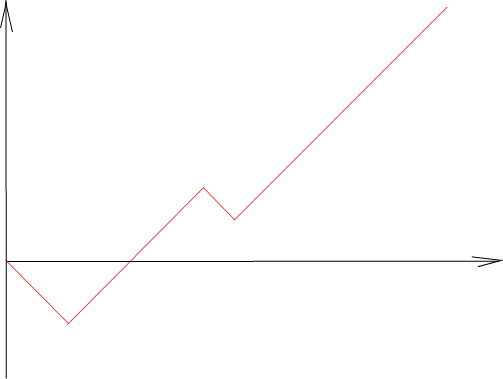
\includegraphics[width=.4\textwidth]{./pictures/4_4.png}
  \caption{График случайноо блуждания}
  \label{fig:44}
\end{figure}

$$S_n =
  \sum \limits_{i = 1}^n \varepsilon_i.$$
Найдём математическое ожидание этого процесса
$$MS_n =
  M \sum \limits_{i = 1}^n \varepsilon_i =$$
Пользуемся независимостью
$$= \sum \limits_{i = 1}^n M \varepsilon_i =
  0,$$
так как
$$M \varepsilon_i =
  1 \cdot \frac{1}{2} - 1 \cdot \frac{1}{2} =
  0.$$
Теперь найдём ковариационную функцию, то есть нужно найти
$$cov \left( S_m, S_t \right) =
  cov \left( \sum \limits_{i = 1}^n \varepsilon_i, \sum \limits_{j = 1}^t \varepsilon_j \right) =$$
Вынесем суммы за ковариацию
$$= \sum \limits_{i = 1}^n \sum \limits_{j = 1}^t cov \left( \varepsilon_i, \varepsilon_j \right) =
\sum \limits_{i, j = 1}^{n, t} M \left( \varepsilon_i \varepsilon_j \right) =$$
Такое математическое ожадине равно
$$M \left( \varepsilon_i \varepsilon_j \right) =
  \begin{cases}
    1, \qquad i = j, \\
    0, \qquad i \neq j.
  \end{cases}$$
Тут пар одинаковых чисел $ \min \left( n, t \right) $, так что
$$= \min \left( n, t \right).$$

По центральной предельной теореме
$$ \frac{S_n}{ \sqrt{n}} \to N \left( 0, 1 \right), \,
  n \to \infty,$$
потому что $S_n$ --- сумма независимых одинаково распределённых случайных величин.

\subsubsection*{4.5}

\textit{Задание.}
Рассмотрим двумерные случайные векторы
$$X^k = \left( \frac{1}{ \sqrt{k}} \cdot S_{ \frac{k}{1}}, \frac{1}{ \sqrt{k}} \cdot S_k \right), \,
  k = 2, 4, 6, \dotsc,$$
где $ \left\{ S_n \right\}_{n \geq 1}$ является простым случайным блужданием.
\begin{enumerate}[label=\alph*)]
  \item Убедитесь, что характеристическая функция вектора $X^k$ имеет вид
  $$ \varphi_{X^k} \left( \theta_1, \theta_2 \right) =
    \left[ \cos \left( \frac{ \theta_1 + \theta_2}{ \sqrt{k}} \right) \right]^{ \frac{k}{2}}
    \left[ \cos \left( \frac{ \theta_2}{ \sqrt{k}} \right) \right]^{ \frac{k}{2}}.$$
  \item Восплользовавшись тем, что
  $$ \varepsilon^{-2} ln \left( \cos \left( \varepsilon \right) \right) \to
    - \frac{1}{2}$$
  при $ \varepsilon \to 0$,
  найдите предел $ \varphi_{X^k} \left( \theta_1, \theta_2 \right) $ при $k \to \infty $
  и укажите распределение случайного вектора $X$,
  к которому слабо сходятся $X^k$ при $k \to \infty$.
\end{enumerate}

\textit{Решение.}
\begin{enumerate}[label=\alph*)]
  \item Сначала нужно найти характеристическую функцию такого вектора
  $ \varphi_{X^{k}} \left( \theta_1, \theta_2 \right) =
    Me^{i \left( \theta_1 X_1^k + \theta_2 X_2^k \right) } $.
  Подставим компоненты
  $$Me^{i \left( \theta_1 X_1^k + \theta_2 X_2^k \right) } =
    Me^{i\left(\theta_1\cdot\frac{1}{\sqrt{k}}\cdot S_{\frac{k}{2}}+\theta_2\cdot\frac{1}{\sqrt{k}}\cdot S_k\right)}.$$
  Можно вынести дробь с корнем от $k$, вместо $S$ будем писать сумму
  $Me^{i\left(\theta_1\cdot\frac{1}{\sqrt{k}}\cdot S_{\frac{k}{2}}+\theta_2\cdot\frac{1}{\sqrt{k}}\cdot S_k\right)} =
    Me^{i\cdot\frac{1}{\sqrt{k}}\left(\theta_1\sum\limits_{i=1}^{\frac{k}{2}}\varepsilon_i +\theta+2\sum\limits_{i = 1}^k\varepsilon_i\right)}$.
  Вторую сумму можно разложить на две
  $$Me^{i\cdot\frac{1}{\sqrt{k}}\left(\theta_1\sum\limits_{i=1}^{\frac{k}{2}}\varepsilon_i +\theta+2\sum\limits_{i = 1}^k\varepsilon_i\right)} =
    Me^{i\cdot\frac{1}{\sqrt{k}}\left(\sum\limits_{i=1}^{\frac{k}{2}}\varepsilon_i\left(\theta_1+\theta_2\right)+\theta_2\sum\limits_{i=\frac{k}{2}+1}^k \varepsilon_i\right)} =$$
  Суммы и слагаемые в суммах независимы
  $$= Me^{i\cdot\frac{1}{\sqrt{k}}\sum\limits_{i=1}^{\frac{k}{2}}\varepsilon_i\left(\theta_1+\theta_2\right)}
    Me^{i \cdot \frac{1}{ \sqrt{k}} \sum \limits_{i = \frac{k}{2} + 1}^k \varepsilon_i \theta_2} =$$
  Все слагаемые в суммах независимы.
  Первое и второе математическое ожидания - произведение $k / 2$ характеристических функций
  \begin{gather*}
    = \prod \limits_{i = 1}^{ \frac{k}{2}}
      \varphi_{ \varepsilon_i} \left( \frac{ \theta_1 + \theta_2}{ \sqrt{k}} \right) \cdot
    \prod \limits_{i = \frac{k}{2} + 1}^k
      \varphi_{ \varepsilon_i} \left( \frac{ \theta_2}{ \sqrt{k}} \right) =
    \end{gather*}
  Осталось понять,
  что такое $ \varphi_{ \varepsilon_i} \left( \lambda \right) = Me^{i \lambda \varepsilon_i}$.
  Случайная величина $ \varepsilon_i$ принимает значения $-1$ и $1$ с вероятностями $0.5$, потому
  $$Me^{i \lambda \varepsilon_i} =
    \frac{1}{2} \cdot e^{i \lambda } + \frac{1}{2} \cdot e^{-i \lambda } =
    \cos \lambda.$$
  Тогда
  $$= \cos^{ \frac{k}{2}} \left( \frac{ \theta_1 + \theta_2}{ \sqrt{k}} \right)
    \cos^{ \frac{k}{2}} \left( \frac{ \theta_2}{ \sqrt{k}} \right).$$
  \item Найдём предел этой характеристической функции, когда $k \to \infty $.

  Оказывается, что
  $$ \varepsilon^{-2} ln \left( \cos \varepsilon \right) \overset{ \varepsilon \to 0}{ \to }
    \frac{1}{2}.$$
  Когда $ \varepsilon \to 0, \, \cos \varepsilon \to 1$ и
  $ln \left( \cos \varepsilon \right) \to 0$ --- это неопределённость 0 на 0.
  Она раскрывается с помощью правила Лопиталя
  $$ \frac{ln \left( \cos \varepsilon \right) }{ \varepsilon^2} \approx
    -\frac{1}{2 \cos \varepsilon } \cdot \frac{ \sin \varepsilon }{ \varepsilon } \to
    \frac{1}{2},$$
  где
  $$ \frac{ \sin \varepsilon }{ \varepsilon }$$
  --- замечательный предел.
  $$ \left( \cos \frac{x}{ \sqrt{k}} \right)^k =
    e^{k \, ln \cos \frac{x}{ \sqrt{k}}} =$$
  Заметим, что
  $$ \frac{x}{ \sqrt{k}} =
    \varepsilon \to
    0,$$
  тогда
  $$= e^{ \frac{k \varepsilon^2 ln \left( \cos \varepsilon \right) }{ \varepsilon^2}} =$$
  Здесь
  $$ \frac{ln \left( \cos \varepsilon \right) }{ \varepsilon^2} \to
    -\frac{1}{2}.$$
  Тогда
  $$= \lim \limits_{ \varepsilon \to 0}
    e^{x^2 \varepsilon^{-2} ln \left( \cos \varepsilon \right) } =
  e^{-\frac{x^2}{2}}.$$
  Теперь нужно эту сходимость использовать
  \begin{gather*}
    \lim \limits_{k \to \infty }
      \cos^{ \frac{k}{2}} \left( \frac{ \theta_1 + \theta_2}{ \sqrt{k}} \right)
      \cos^{ \frac{k}{2}} \left( \frac{ \theta_2}{ \sqrt{k}} \right) =
    e^{-\frac{ \left( \theta_1 + \theta_2 \right)^2}{4}} e^{-\frac{ \theta_2^2}{4}} =
    e^{ \frac{-\theta_1^2 - 2 \theta_1 \theta_2 - \theta_2^2 - \theta_2^2}{4}} = \\
    = e^{-\frac{ \theta_1^2 + 2 \theta_1 \theta_2 + 2 \theta_2^2}{4}}.
  \end{gather*}

  Вывод:
  $$ \varphi_{X^k} \left( \theta_1, \theta_2 \right) \to
    e^{-\frac{1}{4} \left( \theta_1^2 + 2 \theta_1 \theta_2 + 2 \theta_2^2 \right) } =$$
  Это характеристическая функция нормального распределения.
  Оно характеризуется средним и ковариационной матрицей.
  Среднее тут 0, потому что $i$ нет в пределе
  $$= exp \left\{ -\frac{1}{2} \left( A \vec{ \theta }, \vec{ \theta } \right) \right\},$$
  где
  $$ \begin{bmatrix}
      \frac{1}{2} & \frac{1}{2} \\
      \frac{1}{2} & 1
    \end{bmatrix}$$
  --- ковариационная матрица.

  Двумерный случай блуждания сходится к двумерному гауссовскому вектору (рис. \ref{fig:45})
  $$X^k =
    \left( \frac{1}{ \sqrt{k}} \cdot S_{ \frac{k}{2}}, \frac{1}{ \sqrt{k}} \cdot S_k \right) =
    \frac{1}{ \sqrt{k}} \left( S_{k \cdot \frac{1}{2}}, S_{k \cdot 1} \right).$$

  \begin{figure}[h!]
    \centering
    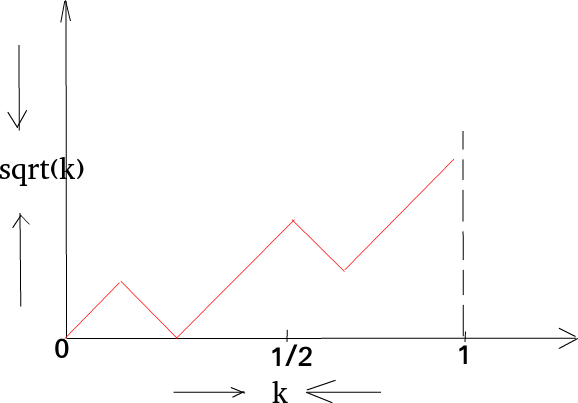
\includegraphics[width=.4\textwidth]{./pictures/4_5.png}
    \caption{Двумерный случай блуждания}
    \label{fig:45}
  \end{figure}

  Если брать не 2 значения, а $n$, то это сходится к
  $$N \left(
      \begin{bmatrix}
        0 \\
        \dotsc \\
        0
      \end{bmatrix},
      \begin{bmatrix}
        t_1 & t_1 & \dotsc & t_1 \\
        \dotsc \\
        t_1 & t_2 & \dotsc & t_n
      \end{bmatrix}
    \right) $$
  --- винеровский процесс.
\end{enumerate}

\subsubsection*{4.6}

\textit{Задание.}
Пусть $ \xi = \left\{ \xi \left( t \right), \, t \geq 0 \right\} $ ---
гауссовский процесс с функцией математического ожидания $m \left( t \right) = t$
и ковариационной функцией
$$K \left( t, s \right) =
  \begin{cases}
    1 - \left| t - s \right|, \qquad \left| t - s \right| < \frac{1}{2}, \\
    \frac{3}{5} - \frac{ \left| t - s \right| }{5}, \qquad \frac{1}{2} \leq \left|t-s\right| < 3, \\
    0, \qquad \left| t - s \right| \geq 3;
  \end{cases}
  t, s \in \mathbb{R}.$$
\begin{enumerate}[label=\alph*)]
  \item Запишите плотность распределения вектора
  $ \left( \xi \left( 1 \right), \xi \left( 3 \right), \xi \left( 4 \right) \right) $.
  \item Найдите условное математическое ожидание
  $M \left(
    \xi \left( 1 \right) \; \middle| \; \left( \xi \left( 3 \right), \xi \left( 4 \right) \right)
  \right) $.
\end{enumerate}

\textit{Решение.}
\begin{enumerate}[label=\alph*)]
  \item Нужно найти плотность трёхмерного вектора
  $ \left( \xi \left( 1 \right), \xi \left( 3 \right), \xi \left( 4 \right) \right) $.
  Процесс гауссовский, значит, такой вектор тоже гауссовский.
  Он характеризуется математическим ожиданием и ковариационной матрицей
  $cov \left( \xi \left( 1 \right), \xi \left( 1 \right) \right) = K \left( 1, 1 \right) $.
  Будем считать по первой строчке.
  Разность равна нулю $K \left( 1, 1 \right) = 1$.
  Аналогично считаем
  $$cov \left( \xi \left( 1 \right), \xi \left( 3 \right) \right) =
    K \left( 1, 3 \right) =
    \frac{1}{5}.$$
  Тогда
  $$ \left( \xi \left( 1 \right), \xi \left( 3 \right), \xi \left( 4 \right) \right)  \sim
    N \left(
      \begin{bmatrix}
        1 \\
        3 \\
        4
      \end{bmatrix},
      \begin{bmatrix}
        1 & \frac{1}{5} & 0 \\
        \frac{1}{5} & 1 & \frac{2}{5} \\
        0 & \frac{2}{5} & 1
      \end{bmatrix}
    \right),$$
  где $cov \left( \xi \left( 1 \right), \xi \left( 4 \right) \right) = K \left( 1, 4 \right) = 0$ и
  $$cov \left( \xi \left( 3 \right), \xi \left( 4 \right) \right) =
    K \left( 3, 4 \right) =
    \frac{2}{5}.$$

  Плотность по определению равна
  $$p \left( \vec{x} \right) =
    \frac{1}{ \sqrt{2 \pi }^3 \sqrt{det \, A}} \cdot
    exp \left\{ -\frac{1}{2}
      \left[ \left( \vec{x} - \vec{m} \right), A^{-1} \left( \vec{x} - \vec{m} \right)
      \right] \right\} =$$
  Чтобы плотность написать, нужно найти определитель матрицы и обратную
  $$det \, A =
    1 - \frac{4}{25} - \frac{1}{5} \cdot \frac{1}{5} =
    \frac{21}{25} - \frac{1}{25} =
    \frac{20}{25} =
    \frac{4}{5}.$$
  Обратная матрица имеет вид
  $$A^{-1} =
    \frac{5}{4}
    \begin{bmatrix}
      \frac{21}{25} & -\frac{1}{5} & \frac{2}{25} \\
      -\frac{1}{5} & 1 & \frac{2}{5} \\
      \frac{2}{25} & \frac{2}{5} & \frac{24}{25}
    \end{bmatrix}.$$
  Тогда плотность равна
  \begin{gather*}
    = \frac{1}{ \sqrt{8 \pi^3 \cdot \frac{4}{5}}} \times \\
    \times exp\{ -\frac{5}{8}
      ( \frac{21}{25} \left( x_1 - 1 \right)^2 + \left( x_2 - 3 \right)^2 +
      \frac{24}{25} \left( x_3 - 4 \right)^2 - \\
      - \frac{2}{5} \left( x_1 - 1 \right) \left( x_2 - 3 \right) +
      \frac{2}{25} \left( x_1 - 1 \right) \left( x_3 - 4 \right) +
      \frac{4}{5} \left( x_2 - 3 \right) \left( x_3 - 4 \right) )\}.
  \end{gather*}

  Здесь
  $$ \vec{x} - \vec{m} =
    \begin{bmatrix}
      x_1 - 1 \\
      x_2 - 3 \\
      x_3 - 4
    \end{bmatrix}.$$
  \item По определению
  $$M \left(
      \xi \left( 1 \right) \; \middle| \; \left( \xi \left( 3 \right), \xi \left( 4 \right) \right)
    \right) =
    \frac{\int\limits_{-\infty}^{+\infty}x_1 p\left(x_1,\xi\left(3\right),\xi\left(4\right)\right)dx_1}{\int\limits_{-\infty}^{+\infty}p\left(x_1,\xi\left(3\right),\xi\left(4\right)\right)dx_1}.$$
  По теореме о нормальной корреляции
  \begin{gather*}
    M \left(
      \xi \left( 1 \right) \; \middle| \; \left( \xi \left( 3 \right), \xi \left( 4 \right) \right)
    \right) = \\
    = M \xi \left( 1 \right) +
    cov_{ \xi \left( 1 \right), \left( \xi \left( 3 \right), \xi \left( 4 \right) \right) } \cdot
    cov_{ \left( \xi \left( 3 \right), \xi \left( 4 \right) \right),
      \left( \xi \left( 3 \right), \xi \left( 4 \right) \right)^{-1}} \cdot
    \begin{bmatrix}
      \xi \left( 3 \right) - M \xi \left( 3 \right) \\
      \xi \left( 4 \right) - M \xi \left( 4 \right)
    \end{bmatrix} =
  \end{gather*}
  Здесь
  $$cov_{ \xi \left( 1 \right), \left( \xi \left( 3 \right), \xi \left( 4 \right) \right) } =
    \begin{bmatrix}
      \frac{1}{5} & 0
    \end{bmatrix}, \,
    cov_{ \left( \xi \left( 3 \right), \xi \left( 4 \right) \right),
      \left( \xi \left( 3 \right), \xi \left( 4 \right) \right)^{-1}} =
    \begin{bmatrix}
      1 & \frac{2}{5} \\
      \frac{2}{5} & 1
    \end{bmatrix}.$$
  Тогда
  \begin{gather*}
    = 1 +
    \begin{bmatrix}
      \frac{1}{5} & 0
    \end{bmatrix}
    \begin{bmatrix}
      1 & \frac{2}{5} \\
      \frac{2}{5} & 1
    \end{bmatrix}^{-1}
    \begin{bmatrix}
      \xi \left( 3 \right) - 3 \\
      \xi \left( 4 \right) - 4
    \end{bmatrix} = \\
    = 1 +
    \begin{bmatrix}
      \frac{1}{5} & 0
    \end{bmatrix} \cdot \frac{25}{21}
    \begin{bmatrix}
      1 & -\frac{2}{5} \\
      \frac{2}{5} & 1
    \end{bmatrix}
    \begin{bmatrix}
      \xi \left( 3 \right) - 3 \\
      \xi \left( 4 \right) - 4
    \end{bmatrix} = \\
    = 1 +
    \begin{bmatrix}
      \frac{5}{21} & 0
    \end{bmatrix}
    \begin{bmatrix}
      \xi \left( 3 \right) - 3 - \frac{2}{5} \cdot \xi \left( 4 \right) + \frac{8}{5} \\
      -\frac{2}{5} \cdot \xi \left( 3 \right) + \frac{6}{5} + \xi \left( 4 \right) - 4
    \end{bmatrix} =
    \frac{5}{21} \cdot \xi \left( 3 \right) - \frac{2}{21} \cdot \xi \left( 4 \right) -
    \frac{2}{3}.
  \end{gather*}
\end{enumerate}

\subsubsection*{4.7}

\textit{Задание.}
Пусть
$$Y_n =
  \sum \limits_{i = 1}^n \xi_i V_i,$$
где $ \left\{ \xi_n \right\}_{n \geq 1}$
является последовательностью независимых одинаково распределённых случайных величин таких, что
$$P \left( \xi_i = 1 \right) =
  P \left( \xi_i = -1 \right) =
  \frac{1}{2},$$
а $ \left\{ V_n \right\}_{n \geq 1}$ является независимой от последовательности
$ \left\{ \xi_n \right\}_{n \geq 1}$
последовательностью независимых одинаково
распределённых случайных величин со стандартным нормальным законом распределения.
\begin{enumerate}[label=\alph*)]
  \item Найдите распределение случайной величины $ \xi_1 V_1$.
  \item Найдите математическое ожидание и ковариационную функцию процесса
  $ \left\{ Y_n, \, n \geq 1 \right\} $.
  \item Докажите, что процесс $ \left\{ Y_n, \, n \geq 1 \right\} $ имеет независимые приращения.
  Найдите распределение приращений.
  \item Докажите, что процесс $ \left\{ Y_n, \, n \geq 1 \right\} $ является гауссовским.
  \item Запишите совместную плотность распределения $f_{Y_n, Y_{2n}} \left( x, y \right) $
  случайных величин $Y_n$ и $Y_{2n}$.
\end{enumerate}

\textit{Решение.}
\begin{enumerate}[label=\alph*)]
  \item $ \xi_1 V_1$ --- это произведение нормальной величины на бернуллиевскую, они независимы.

  Найдём характеристическую функцию такого произведения
  $$ \varphi_{ \xi_1 V_1} \left( t \right) =
    Me^{it \xi_1 V_1} =$$
  Переберём значения $ \xi_1$.
  Имеем
  $$= M \left(
    e^{itV_1} \cdot \mathbbm{1} \left\{ \xi_1 = 1 \right\} +
    e^{-itV_1} \cdot \mathbbm{1} \left\{ \xi_1 = -1 \right\} \right) =$$
  Пользуемся независимостью
  $$= Me^{itV_1} \cdot P \left( \xi_1 = 1 \right) + Me^{-itV_1} \cdot P \left( \xi_1 = -1 \right).$$
  Математическое ожидание --- это характеристическая функция стандартного нормального распределия
  $$Me^{itV_1} \cdot P \left( \xi_1 = 1 \right) + Me^{-itV_1} \cdot P \left( \xi_1 = -1 \right) =
    e^{-\frac{t^2}{2}} \cdot \frac{1}{2} + e^{-\frac{t^2}{2}} \cdot \frac{1}{2} =
    e^{-\frac{t^2}{2}}.$$
  Получилось такое же распределение $ \xi_1 V_1 \sim N \left( 0, 1 \right) $.

  Случайные величины $V_1$ и $-V_1$ имеют одинаковое распределение,
  потому что плотность симметрична $z_i = \xi_i V_i \sim N \left( 0, 1 \right) $,
  при этом $z_1, z_2, \dotsc $ --- независимы и
  $$Y_n =
    \sum \limits_{i = 1}^n z_i.$$
  \item Найдём математическое ожидание процесса
  $$MY_n =
    M \sum \limits_{i = 1}^n z_i =$$
  Пользуемся независимостью
  $$= \sum \limits_{i = 1}^n Mz_i =
    0.$$
  Ищем ковариационную функцию процесса
  $$K \left( Y_n, Y_m \right) =
    cov \left( Y_n, Y_m \right) =
    cov \left( \sum \limits_{i = 1}^n z_i, \sum \limits_{j = 1}^m z_j \right) =
    \sum \limits_{i = 1}^n \sum \limits_{j = 1}^m cov \left( z_i, z_j \right) =$$
  При $i \neq j \qquad cov \left( z_i, z_j \right) = 0$,
  при $i = j \qquad cov \left( z_i, z_i \right) = Dz_i = 1$.
  Двойная сумма --- это количество пар с одинаковыми индексами
  $$= min \left( n, m \right).$$
  \item Запишем приращения $Y_n$, то есть $Y_{n_1}, Y_{n_2} - Y_{n_1}, Y_{n_3} - Y_{n_2}, \dotsc $,
  индексы $1 \leq n_1 \leq n_2 < n_3 < \dotsc $.
  Запишем через суммы
  $$Y_{n_1}, Y_{n_2} - Y_{n_1}, Y_{n_3} - Y_{n_2}, \dotsc  =
    \sum \limits_{i = 1}^{n_1} z_i,
    \sum \limits_{i = n_1 + 1}^{n_2} z_i,
    \sum \limits_{i = n_2 + 1}^{n_3} z_i, \dotsc.$$
  В каждой такой сумме разные $z$, они независимы, следовательно, приращения независимы.

  Пусть
  $$Y_n - Y_m =
    \sum \limits_{i = m + 1}^n z_i \sim $$
  Сумма независимых нормальных величин --- это тоже нормальная величина
  $$ \sim N \left( 0, n - m \right).$$
  \item Процесс гауссовский, если линейная комбинация
  $$ \sum \limits_{r = 1}^k c_r \cdot I_{n_k} =$$
  --- гауссовские.
  Перепишем через приращения
  $$= \sum \limits_{r = 1}^n d_r \left( Y_{n_r} - Y_{n_{r - 1}} \right).$$
  В такой сумме разности гауссовские и независимы.

  Значит и процесс будет гауссовским.
  \item $$f_{Y_n, Y_{2n}} \left( x, y \right) =
    \frac{1}{2 \pi n} \cdot exp \left\{ -\frac{1}{2n} \left( 2x^2 - 2xy + y^2 \right) \right\}.$$

  Ковариация --- это матрица из минимумов
  $$cov_{\begin{bmatrix} Y_n \\ Y_{2n} \end{bmatrix}, \begin{bmatrix} Y_n \\ Y_{2n} \end{bmatrix}} =
    \begin{bmatrix}
      n & n \\
      n & 2n
    \end{bmatrix} =
    A.$$

  Определитель этой матрицы $det \, A = 2n^2 - n^2 = n^2$.

  Обратная матрица
  $$A^{-1} =
    \frac{1}{n^2}
    \begin{bmatrix}
      2n & -n \\
      -n & n
    \end{bmatrix} =
    \frac{1}{n}
    \begin{bmatrix}
      2 & -1 \\
      -1 & 1
    \end{bmatrix}.$$
\end{enumerate}

\subsubsection*{4.8}

\textit{Задание.}
Пусть $X$ и $Y$ являются независимыми случайными велчинами,
причём $Y$ имеет равномерное распределение на отрезке $ \left[ 0, 2 \pi \right] $,
а $X$ имеет плотность распределения
$f_X \left( x \right) =
  xe^{-\frac{x^2}{2}} \mathbbm{1} \left\{ x \geq 0 \right\} $.
\begin{enumerate}[label=\alph*)]
  \item Докажите, что случайные величины $X \cos Y, \, X \sin Y$
  являются независимыми и имеют стандартное нормальное распределение.
  \item Докажите, что процесс
  $ \xi \left( t \right) = X \cos \left( 2 \pi t + Y \right), \,
    t \in \mathbb{R}$
  является гауссовским.
  Найдите его математическое ожидание и ковариационную функцию.
\end{enumerate}

\textit{Решение.}
\begin{enumerate}[label=\alph*)]
  \item Нужно доказать, что $X \cos Y$ и $X \sin Y$ ---
  независимые с распределением $N \left( 0, 1 \right) $,
  то есть нужно описать распределение двух таким величин.

  Найдём характеристическую функцию
  \begin{gather*}
    \varphi_{ \left( X \cos Y, \, X \sin Y \right) } \left( \theta_1, \theta_2 \right) =
    M \, exp \left\{ i \left( \theta_1 X \cos Y + \theta_2 X \sin Y \right) \right\} = \\
    = \int \limits_0^{ \infty }
      \int \limits_{0}^{2 \pi }
        e^{i \left( \theta_1 x \cos y + \theta_2 x \sin y \right) } \cdot \frac{1}{2 \pi } \cdot
        xe^{-\frac{x^2}{2}} dydx =
  \end{gather*}
  Это двойной интеграл, записанный в полярных координатах
  $$u = x \cos y, \,
    v = x \sin y, \,
    dudv = xdxdy.$$
  Получаем
  $$= \int \limits_{-\infty }^{+\infty }
    \int \limits_{-\infty }^{+\infty }
      e^{i \left( \theta_1 u + \theta_2 v \right) } \cdot \frac{1}{2 \pi } \cdot
      e^{-\frac{u^2}{2}} \cdot e^{-\frac{v^2}{2}} dudv =$$
  Здесь
  $$ \frac{1}{2 \pi } \cdot e^{-\frac{u^2}{2}} \cdot e^{-\frac{v^2}{2}}$$ ---
  это совместная плотность $ \left( X \cos Y, \, X \sin Y \right) $ ---
  это произведение стандартных плотностей
  $$= e^{-\frac{ \theta_1^2}{2} - \frac{ \theta_2^2}{2}},$$
  то есть такие две величины --- это независимые стандартные гауссовские случайные величины.
  \item $ \xi \left( t \right) = X \cos \left( 2 \pi t + Y \right) $.
  Распишем косинус суммы
  \begin{gather*}
    X \cos \left( 2 \pi t + Y \right) =
    X \cos \left( 2 \pi t \right) \cos Y - X \sin \left( 2 \pi t \right) \sin Y = \\
    = \cos \left( 2 \pi t \right) \left( X \cos Y \right) -
    \sin \left( 2 \pi t \right) \left( X \sin Y \right),
  \end{gather*}
  следовательно, $ \xi $ --- гауссовский процесс.

  Нужно проверять, что любые суммы
  $$ \sum \limits_{r = 1}^k c_r \xi \left( t_r \right) =
    \alpha \cdot X \cos Y + \beta X \sin Y$$
  --- гауссовская величина, где $X \cos Y, \, X \sin Y$ --- независимые гауссовские величины.

  Математическое ожидание
  \begin{gather*}
    M \xi \left( t \right) =
    M \left[
      \cos \left( 2 \pi t \right) \left( X \cos Y \right) -
      \sin \left( 2 \pi t \right) \left( X \sin Y \right) \right] = \\
    = \cos \left( 2 \pi t \right) M \left( X \cos Y \right) -
    \sin \left( 2 \pi t \right) M \left( X \sin Y \right) =
    0.
  \end{gather*}

  Ковариационная функция
  \begin{gather*}
    K \left( \xi \left( t \right), \xi \left( s \right) \right) =
    M \left[ \xi \left( t \right) \xi \left( s \right) \right] -
    M \xi \left( t \right) \cdot M \xi \left( s \right) = \\
    = M \left[ X \cos \left( 2 \pi t + Y \right) X \cos \left( 2 \pi s + Y \right) \right] - \\
    - M \left[ X \cos \left( 2 \pi t + Y \right) \right]
    M \left[ X \cos \left( 2 \pi s + Y \right) \right] = \\
    = M\{ \left[
      \cos \left( 2 \pi t \right) \left( X \cos Y \right) -
      \sin \left( 2 \pi s \right) \left( X \sin Y \right) \right] \times \\
      \times \left[ \cos \left( 2 \pi s \right) \left( X \cos Y \right) -
      \sin \left( 2 \pi s \right) \left( X \sin Y \right) \right] \} - \\
    - M \left[
      \cos \left( 2 \pi t \right) \left( X \cos Y \right) -
      \sin \left( 2 \pi t \right) \left( X \sin Y \right) \right] \times \\
    \times M \left[ \cos \left( 2 \pi s \right) \left( X \cos Y \right) -
      \sin \left( 2 \pi s \right) \left( X \sin Y \right) \right] = \\
    = M[
      \cos \left( 2 \pi t \right) \cos \left( 2 \pi s \right) \left( X \cos Y \right)^2 - \\
      - \cos \left( 2 \pi t \right) \sin \left( 2 \pi s \right) X \cos Y \cdot X \sin Y - \\
      - \sin \left( 2 \pi t \right) \cos \left( 2 \pi s \right) X \sin Y \cdot X \cos Y +
      \sin \left( 2 \pi t \right) \sin \left( 2 \pi s \right) \left( X \sin Y \right)^2 ] = \\
    = \cos \left( 2 \pi t \right) \cos \left( 2 \pi s \right) +
    \sin \left( 2 \pi t \right) \sin \left( 2 \pi s \right) =
    \cos \left[ 2 \pi \left( t - s \right) \right].
  \end{gather*}
\end{enumerate}

\addcontentsline{toc}{section}{Домашнее задание}
\section*{Домашнее задание}

\subsubsection*{4.10}

\textit{Задание.}
Выясните, существует ли случайный процесс с ковариационной функцией
\begin{enumerate}[label=\alph*)]
  \item $K \left( t, s \right) = \min \left( t, s \right) - ts, \, t, s \in \left[ 0, 1 \right] $;
  \item $K \left( t, s \right) = e^{- \left| t - s \right| }, \, t, s \in \mathbb{R}$.
\end{enumerate}

\textit{Решение.}
\begin{enumerate}[label=\alph*)]
  \item $K \left( t, s \right) = \min \left( t, s \right) - ts, \, t, s \in \left[ 0, 1 \right] $.

  Такой процесс есть.
  Это броуновский мост;
  \item $K \left( t, s \right) = e^{- \left| t - s \right| }, \, t, s \in \mathbb{R}$.

  Симметричность очевидна.
  Вопрос: буде ли такая функция неотрицательно определена?

  Функция зависит только от разности.
  Сейчас $K \left( t, s \right) = \varphi \left( t - s \right) $,
  где $ \varphi \left( t \right) = e^{-\left| t \right| }, \, t \in \mathbb{R}$.

  Так что
  $$ \sum \limits_{k, j = 1}^n c_k c_j K \left( t_k, t_j \right) =
    \sum \limits_{k, j = 1}^n c_k c_j \varphi \left( t_k - t_j \right) \geq
    0$$
  --- это условие неотрицательной определённости для характеристической функции.
  Будет ли эта функция $ \varphi $ характеристической?
  То есть вопрос в задаче равносилен следующему:
  будет ли $ \varphi \left( t \right) = e^{-\left| t \right| }, \, t \in \mathbb{R}$
  характеристической функцией?
  Это характеристическая функция для распределения Коши.
\end{enumerate}

\subsubsection*{4.11}

\textit{Задание.}
Докажите, что функция $K \left( t, s \right) = e^{ts}$
является ковариационной функцией некоторого случайного процесса.

\textit{Решение.}
Симметричность есть.
Вопрос: будет ли такая функция неотрицательно определёной
$$ \sum \limits_{k, j = 1}^n c_k c_j K \left( t_k, t_j \right) =
  \sum \limits_{k, j = 1}^n c_k c_j e^{t_k t_j} =
  \sum \limits_{k, j = 1}^n \left( \sum \limits_{i = 0}^{ \infty } \frac{t_k^i t_j^i}{i!} \right) =
  \sum \limits_{i = 0}^{ \infty } \frac{1}{i!} \sum \limits_{k, j = 1}^n c_k c_j t_k^i t_j^i =$$
Разобьём двойную сумму на две
$$= \sum \limits_{i = 0}^{ \infty } \frac{1}{i!} \sum \limits_{k = 1}^n c_k t_k^i
  \sum \limits_{j = 1}^n c_j t_j^i =
  \sum \limits_{i = 0}^{ \infty } \frac{1}{i!} \left( \sum \limits_{k = 1}^n c_k t_k \right)^i \geq
  0,$$
следовательно, $K \left( t, s \right) = e^{ts}$ --- ковариационная функция.

\subsubsection*{4.12}

\textit{Задание.}
Пусть $ \varphi_1, \dotsc, \varphi_n$ --- произвольные действительные функции,
$c_1, \dotsc, c_n$ --- неотрицательные числа.
Докажите, что функция
$$K \left( t, s \right) =
  \sum \limits_{i = 1}^n c_i \varphi_i \left( t \right) \varphi_i \left( s \right) $$
является ковариационной функцией некоторого случайного процесса.

\textit{Решение.}
Симметричность очевидна.
Вопрос: будет ли такая функция неотрицательно определённой?
$$ \sum \limits_{k, j = 1}^n \lambda_k \lambda_j \sum \limits_{i = 1}^n K \left( t_k, t_j \right) =
  \sum \limits_{k, j = 1}^n \lambda_k \lambda_j
  \sum \limits_{i = 1}^n c_i \varphi_i \left( t_k \right) \varphi_i \left( t_j \right) =$$
Поменяем суммы местами и двойную сумму распишем как две отдельные
$$= \sum \limits_{i = 1}^n c_i \sum \limits_{k = 1}^n \lambda_k \varphi_i \left( t_k \right)
  \sum \limits_{j = 1}^n \lambda_j \varphi_i \left( t_j \right) =
  \sum \limits_{i = 1}^n c_i
    \sum \limits_{k = 1}^n \left( \lambda_k \varphi_i \left( t_k \right) \right)^2 \geq
  0.$$

Значит, функция ковариационная.


\subsubsection*{4.13}

\textit{Задание.}
Пусть случайные величины $X$ и $Y$ имеют совместное гауссовское распределение.
Докажите, что процесс $ \xi \left( t \right) = tX + y, \, t \geq 0$ гауссовский.
Найдите его математическое ожидание и ковариационную функцию.

\textit{Решение.}
$ \xi \left( t \right) $ --- гауссовский, если
$$ \forall \vec{ \alpha } \in \mathbb{R}^n \qquad
  \left( \vec{ \alpha }, \vec{ \xi } \right) = \sum \limits_{i = 1}^n \alpha_i \xi_i$$
--- гауссовская случайная величина, то есть
$$ \sum \limits_{i = 1}^n \xi \left( t_i \right) \alpha_i =
  \sum \limits_{i = 1}^n \left( t_i X + Y \right) \alpha_i =
  X \sum \limits_{i = 1}^n t_i \alpha_i + Y \sum \limits_{i = 1}^n \alpha_i$$
--- сумма гауссовских случайных величин, гауссовская, $ \forall t_1, \dotsc, t_n \geq 0$.

Математическое ожидание $M \xi \left( t \right) = M \left( tX + Y \right) = tMX + My$.

Ковариационная функция
\begin{gather*}
  K \left( t, s \right) = \\
  = M \left[ \xi \left( t \right) \xi \left( s \right) \right] -
  M \xi \left( t \right) M \xi \left( s \right)
  M \left[ \left( tX + Y \right) \left( sX + Y \right) \right] - \\
  - M \left( tX + Y \right) M \left( sX + Y \right) = \\
  = tsMX^2 + tM \left( XY \right) + sM \left( XY \right) + MY^2 -
  \left( tMX + MY \right) \left( sMX + MY \right) = \\
  = tsMX^2 + \left( t + s \right) M \left( XY \right) + MY^2 - ts \left( MX \right)^2 -
  tMX \cdot MY - sMY \cdot MX - \\
  - \left( MY \right)^2 =
  tsDX + DY + \left( t + s \right) D \left( XY \right).
\end{gather*}

\subsubsection*{4.14}

\textit{Задание.}
Пусть $ \left\{ S_n, \, n = 0, 1, 2, \dotsc \right\} $ является случайным блужданием,
которое определяется следующим образом: $S_0 = 0; \, S_{n + 1} = S_n + \xi_{n + 1}$,
где $ \left\{ \xi_n \right\}_{n \geq 1}$ ---
последовательность независимых одинаково распределённых случайных величин таких,
что $M \left[ \xi \right] = 0, \, M \left[ \xi^2 \right] = 1$.
Докажите, что для произвольного фиксированного
$$t \in \left[ 0, 1 \right] \qquad
  \frac{S_{ \left[ nt \right] }}{ \sqrt{n}} \overset{d}{ \to } N \left( 0, t \right), \,
  n \to \infty.$$

\textit{Решение.}
\begin{gather*}
  S_1 = S_0 + \xi_1 = 0 + \xi_1 = \xi_1, \\
  S_2 = S_1 + \xi_2 = \xi_1 + \xi_2, \\
  S_3 = S_2 + \xi_3 = \xi_1 + \xi_2 + \xi_3, \\
  \dotsc, \\
  S_n = \sum \limits_{i = 1}^n \xi_i.
\end{gather*}

Математическое ожидание
$$MS_n =
  M \sum \limits_{i = 1}^n \xi_i =
  \sum \limits_{i = 1}^n M \xi_i =
  nM \xi_i =
  0.$$

Дисперсия
$$DS_n =
  D \sum \limits_{i = 1}^n \xi_i =
  \sum \limits_{i = 1}^n D \xi_i =
  nD \xi_i =
  n.$$

Значит, по центральной предельной теореме
$$ \frac{S_{ \left[ nt \right] }}{ \sqrt{n}} \overset{d}{ \to } N \left( 0, t \right), \,
  n \to \infty.$$

\subsubsection*{4.16}

\textit{Задание.}
Пусть $ \xi = \left\{ \xi \left( t \right), \, t \geq 0 \right\} $ ---
гауссовский процесс с нулевым математическим ожиданием и ковариационной функцией
$$K \left( t, s \right) =
  \begin{cases}
    1 - \left| t - s \right|, \qquad \left| t - s \right| < \frac{1}{2}, \\
    \frac{2}{3} - \frac{ \left| t - s \right| }{3}, \qquad
    \frac{1}{2} \leq \left| t - s \right| < 2, \\
    0, \qquad \left| t - s \right| \geq 2.
  \end{cases}; \, t, s \in \mathbb{R}$$
\begin{enumerate}[label=\alph*)]
  \item Запишите плотноть распределения вектора
  $ \left( \xi \left( 4 \right), \xi \left( 5 \right), \xi \left( 6 \right) \right) $.
  \item Найдите условное математическое ожидание
  $M \left(
    \xi \left( 5 \right) \; \middle| \; \left( \xi \left( 4 \right), \xi \left( 6 \right) \right)
  \right) $.
\end{enumerate}

\textit{Решение.}
$M \left( t \right) =
  0$.
\begin{enumerate}[label=\alph*)]
  \item Нужно найти плотность трёхмерного вектора
  $ \left( \xi \left( 4 \right), \xi \left( 5 \right), \xi \left( 6 \right) \right) $.

  Процесс гауссовский, значит, такой вектор тоже гауссовский.
  Он характеризуется математическим ожадинием и ковариационной матрицей
  $cov \left[ \xi \left( 4 \right), \xi \left( 4 \right) \right] =
    cov \left[ \xi \left( 5 \right), \xi \left( 5 \right) \right] =
    cov \left[ \xi \left( 6 \right), \xi \left( 6 \right) \right] =
    K \left( 4, 4 \right) $.
  Будем считать по первой строке.
  Разность равна нулю $K \left( 4, 4 \right) = 1$.

  Аналогично считаем
  $$cov \left[ \xi \left( 4 \right), \xi \left( 3 \right) \right] =
    K \left( 4, 5 \right) =
    \frac{2}{3} - \frac{1}{3} =
    \frac{1}{3}.$$
  По последней строке находим,
  что $cov \left[ \xi \left( 4 \right), \xi \left( 6 \right)\right] = K \left( 4, 6 \right) = 0$, а
  $$cov \left[ \xi \left( 5 \right), \xi \left( 6 \right) \right] =
    K \left( 5, 6 \right) =
    \frac{2}{3} - \frac{1}{3} =
    \frac{1}{3}.$$

  Тогда распределение вектора имеет вид
  $$ \left( \xi \left( 4 \right), \xi \left( 5 \right), \xi \left( 6 \right) \right) \sim
    N \left(
      \begin{bmatrix}
        0 \\
        0 \\
        0
      \end{bmatrix},
      \begin{bmatrix}
        1 & \frac{1}{3} & 0 \\
        \frac{1}{3} & 1 & \frac{1}{3} \\
        0 & \frac{1}{3} & 1
      \end{bmatrix}
    \right).$$

  Плотность имеет вид
  $$p \left( \vec{x} \right) =
    \frac{1}{ \sqrt{2 \pi}^3 \sqrt{det \, A}} \cdot
    exp \left\{
      -\frac{1}{2} \left[ \left( \vec{x} - \vec{m} \right),
      A^{-1} \left( \vec{x} - \vec{m} \right) \right] \right\} =$$
  Чтобы написать плотность, нужно найти определитель матрицы и обратную
  $$det \, A =
    \begin{vmatrix}
      1 & \frac{1}{3} & 0 \\
      \frac{1}{3} & 1 & \frac{1}{3} \\
      0 & \frac{1}{3} & 1
    \end{vmatrix} =
    \begin{vmatrix}
      1 & \frac{1}{3} \\
      \frac{1}{3} & 1
    \end{vmatrix} -
    \frac{1}{3} \begin{vmatrix}
      \frac{1}{3} & \frac{1}{3} \\
      0 & 1
    \end{vmatrix} =
    1 - \frac{1}{9} - \frac{1}{3} \cdot \frac{1}{3} =
    1 - \frac{1}{9} - \frac{1}{9} =
    \frac{7}{9}.$$
  Обратная матрица
  $$A^{-1} =
    \frac{9}{7}
    \begin{bmatrix}
      \frac{8}{9} & -\frac{1}{3} & \frac{1}{9} \\
      -\frac{1}{3} & 1 & -\frac{1}{3} \\
      \frac{1}{9} & -\frac{1}{3} & \frac{8}{9}
    \end{bmatrix}.$$
  Подставим определитель и обратную матрицу в выражение для плотности
  \begin{gather*}
    = \frac{1}{ \sqrt{8 \pi^3 \cdot \frac{7}{9}}} \times \\
    \times exp \left\{
      -\frac{9}{14} \left( \frac{8}{9} \cdot x_1^2 - \frac{2}{3} \cdot x_1 x_2 +
      \frac{2}{9} \cdot x_1 x_3 + x_2^2 + \frac{8}{9} \cdot x_3^2 - \frac{2}{3} \cdot x_2 x_3 \right)
    \right\}.
  \end{gather*}

  Здесь
  $$ \vec{x} - \vec{m} =
    \begin{bmatrix}
      x_1 \\
      x_2 \\
      x_3
    \end{bmatrix}.$$
  \item По определению условного математического ожидания
  $$M \left(
      \xi \left( 5 \right) \; \middle| \; \left( \xi \left( 4 \right), \xi \left( 6 \right) \right)
    \right) =
    \frac{\int\limits_{-\infty}^{+\infty}x_2 p\left(\xi\left(4\right),x_2,\xi\left(6\right)\right)dx_2}{\int\limits_{-\infty}^{+\infty}p\left(\xi\left(4\right),x_2,\xi\left(6\right)\right)dx_2.}$$

  Теорема о нормальной корреляции
  \begin{gather*}
    M \left(
      \xi \left( 5 \right) \; \middle| \; \left( \xi \left( 4 \right), \xi \left( 6 \right) \right)
    \right) = \\
    = M \xi \left( 5 \right) +
    cov_{ \xi \left(5 \right), \left( \xi \left( 4 \right), \xi \left( 6 \right) \right) } \cdot
    cov_{\left(\xi\left(4\right),\xi\left(6\right)\right),\left(\xi\left(4\right),\xi\left(6\right)\right)^{-1}} \cdot
    \begin{bmatrix}
      \xi \left( 4 \right) - M \xi \left( 4 \right) \\
      \xi \left( 6 \right) - M \xi \left( 6 \right)
    \end{bmatrix} =
  \end{gather*}
  Здесь
  Первая ковариация равна
  $$ \begin{bmatrix}
    \frac{1}{3} & \frac{1}{3}
  \end{bmatrix},$$
  а вторая ---
  $$ \begin{bmatrix}
    1 & 0 \\
    0 & 1
  \end{bmatrix}.$$
  Тогда
  $$= \begin{bmatrix}
    \frac{1}{3} & \frac{1}{3}
  \end{bmatrix}
  \begin{bmatrix}
    1 & 0 \\
    0 & 1
  \end{bmatrix}
  \begin{bmatrix}
    \xi \left( 4 \right) \\
    \xi \left( 6 \right)
  \end{bmatrix} =
  \begin{bmatrix}
    \frac{1}{3} & \frac{1}{3}
  \end{bmatrix}
  \begin{bmatrix}
    \xi \left( 4 \right) \\
    \xi \left( 6 \right)
  \end{bmatrix} =
  \frac{1}{3} \left[ \xi \left( 4 \right) + \xi \left( 6 \right) \right].$$
\end{enumerate}

\addcontentsline{toc}{chapter}{Занятие 5. Винеровский процесс}
\chapter*{Занятие 5. Винеровский процесс}

\addcontentsline{toc}{section}{Контрольные вопросы и задания}
\section*{Контрольные вопросы и задания}

\subsubsection*{Приведите определение винеровского процесса.}

$ \left\{ w \left( t \right), \, t \geq 0 \right\} $ --- винеровский процесс,
если обладает рядом свойств:
\begin{enumerate}
  \item $w \left( 0 \right) = 0$;
  \item однородные приращения.
  Рассмотрим приращение винеровского процесса на $t$.
  Тогда
  $w \left( s + t \right) - w \left( s \right) \overset{def}{=}
    w \left( t \right) \sim
    N \left( 0, t \right) $, то есть распределение процесса зависит только от длины отрезка;
  \item независимые приращения на непересекающихся отрезках.
  Выберем $0 < t_1 < t_2 < \dotsc < t_n$.
  Тогда
  $w \left( t_1 \right), \,
    w \left( t_2 \right) - w \left( t_1 \right),
    \dotsc,
    w \left( t_n \right) - w \left( t_{n - 1} \right) $ ---
  независимые в совокупности случайные величины.
\end{enumerate}

\subsubsection*{Запишите плотность винеровского процесса.}

Напишем плотность распределения вектора
$ \left( w \left( t_1 \right), \dotsc, w \left( t_n \right) \right) =
  \vec{ \xi }$.

Будем использовать матрицу
$$A =
  \begin{bmatrix}
    1 & 0 & 0 & 0 & \dotsc & 0 \\
    1 & 1 & 0 & 0 & \dotsc & 0 \\
    1 & 1 & 1 & 0 & \dotsc & 0 \\
    \dotsc \\
    1 & 1 & 1 & 1 & \dotsc & 1
  \end{bmatrix}.$$

Таким образом $ \vec{ \xi }$ имеет плотность
$$q \left( A^{-1} \vec{u} \right) =
  \prod \limits_{j = 0}^{n - 1}
    \frac{1}{ \sqrt{2 \pi \left( t_{j + 1} - t_j \right) }} \cdot e^{-\frac{u_{j + 1} - u_j}{2t_{j + 1} - t_j}}.$$
В этой плотности считаем, что $t_0 = 0, \, u_0 = 0$.

\subsubsection*{Запишите ковариационную функцию винеровского процесса.}

Произведение математических ожиданий --- это 0, потому
$$K \left( t, s \right) =
  Mw \left( s \right) w \left( t \right) =$$
Используем независимость приращений
$$= M \left\{
    w \left( s \right) \cdot
    \left[ w \left( s \right) + \left( w \left( t \right) - w \left( s \right) \right) \right]
  \right\} =$$
Раскрываем скобки
$$= M \left\{
    w^2 \left(s \right) + Mw \left( s \right) \left[ w \left( t \right) - w \left( s \right) \right]
  \right\} =$$
Первое слагаемое равно $s$, а второе --- нулю,
так как это независимые центрированные случайные величины (математическое произведения ---
это произведение математических ожиданий, а они равны нулю)
$$= s, \,
  s < t.$$

$K \left( t, s \right) = \min \left( s, t \right) $.

\addcontentsline{toc}{section}{Аудиторные задачи}
\section*{Аудиторные задачи}

\subsubsection*{5.2}

\textit{Задание.}
Пусть $ \left\{ W \left( t \right), \, t \geq 0 \right\} $ --- винеровский процесс.
Докажите, что
$M \left( W \left( t \right) - W \left( s \right) \right)^{2n + 1} = 0, \,
  M \left( W \left( t \right) - W \left( s \right) \right)^{2n} =
  \left( 2n - 1 \right)!! \left( t - s \right)^n$.

\textit{Решение.}
Приращение гауссовское.
Обозначим
$$ \xi =
  W \left( t \right) - W \left( s \right) \overset{def}{=}
  W \left( t - s \right).$$
Значит, $ \xi \sim N \left( 0, t - s \right) $, где $t - s = \sigma^2$.
Нужны формулы для моментов центрированной гауссовской случайной величины, то есть
Знаем, что $M \xi^{2n + 1} = 0, \, M \xi^{2n} = \left( 2n + 1 \right)!! \sigma^{2n}$.

\subsubsection*{5.3}

\textit{Задание.}
Пусть $ \left\{ W \left( t \right), \, t \geq 0 \right\} $ --- винеровский процесс.
Вычислите:
\begin{enumerate}[label=\alph*)]
  \item $M \left[ \left( W \left( 5 \right) - 2W \left( 1 \right) + 2 \right)^3 \right] $;
  \item характеристическую функцию случайной величины $W \left( 2 \right) + 2W \left( 1 \right) $;
  \item $M \left[ \sin \left( 2W \left( 1 \right) + W \left( 2 \right) \right) \right] $;
  \item $M \left[ \cos \left( 2W \left( 1 \right) + W \left( 2 \right) \right) \right] $.
\end{enumerate}

\textit{Решение.}
Есть винеровский процесс.
\begin{enumerate}[label=\alph*)]
  \item $W \left( 5 \right) - 2W \left( 1 \right) + 2 = \xi \sim N \left( 2, 5 \right) $,
  потому что это линейная комбинация элементов гауссовского вектора.
  Найдём дисперсию.
  Константа на неё не влияет
  $$D \xi =
    D \left[ W \left( 5 \right) - 2W \left( 1 \right) \right] =
    cov \left( \xi, \xi \right) =$$
  Подставим выражения для случайной величины
  $$= cov \left[ W \left( 5 \right) - 2W \left( 1 \right) + 2, \,
      W \left( 5 \right) - 2W \left( 1 \right) + 2 \right] =$$
  Воспользуемся линейностью
  $$= K \left( 5, 5 \right) - 2K \left( 5, 1 \right) - 2K \left( 5, 1 \right) +
    4K \left( 1, 1 \right) =
    5 - 2 - 2 + 4 =
    5.$$
  Нужно найти третий момент.
  $ \xi $ не центрирована.
  Нужно её центрировать $M \xi^3 = M \left[ \left( \xi - 2 \right) + 2 \right]^3 $.
  Раскрываем скобки
  $$M \xi^3 =
    M \left( \xi - 2 \right)^3 + 6M \left( \xi - 2 \right)^3 + 12M \left( \xi - 2 \right) + 8.$$
  По предыдущей задаче первое слагаемое --- 0, так как величина центрирована, второй момент --- 5,
  так как это дисперсия, первый момент --- 0.
  Тогда $M \xi^3 = 0 + 6 \cdot 5 + 12 \cdot 0 + 8 = 38$.

  Величины $W \left( 5 \right) $ и $W \left( 1 \right) $ --- зависимы,
  а приращения в винеровском процессе --- независимы, потому имеем сумму дисперсий
  $$D \left[ W \left( 5 \right) - 2W \left( 1 \right) \right] =
    D \left\{
      \left[ W \left( 5 \right) - W \left( 1 \right) \right] + \left[ -W \left( 1 \right) \right]
    \right\}.$$
  Дисперсия первого слагаемого равна 4, а второго --- 1.
  Слагаемые независимы $D \left[ W \left( 5 \right) - 2W \left( 1 \right) \right] = 5$;
  \item нужно найти характеристическую функцию $W \left( 2 \right) + 2W \left( 1 \right) $.

  Математическое ожидание такой величины равно нулю, а дисперсия
  $D \left[ W \left( 2 \right) + 2W \left( 1 \right) \right] =
    D \left\{
      \left[ W \left( 2 \right) - W \left( 1 \right) \right] + 3W \left( 1 \right)
    \right\}$.
  Это независимые величины, поэтому
  $D \left\{
      \left[ W \left( 2 \right) - W \left( 1 \right) \right] + 3W \left( 1 \right)
    \right\} =
    1 + 9 = 10$.
  Значит, получается
  $ \varphi_{W \left( 2 \right) + 2W \left( 1 \right) } \left( \lambda \right) =
    \varphi_{N \left( 0, 10 \right) } \left( \lambda \right) =
    e^{-\frac{10 \lambda^2}{2}}$;
  \item $M \left[ \sin \left( 2W \left( 1 \right) + W \left( 2 \right) \right) \right] = 0$.

  Характеристическая функция случайной величины --- это
  $$ \varphi_{ \xi } \left( \lambda \right) = Me^{i \lambda \xi } =
    M \cos \lambda \xi + iM \sin \lambda \xi, \,
    \lambda = 1;$$
  \item $M \left[ \cos \left( 2W \left( 1 \right) + W \left( 2 \right) \right) \right] = e^{-5}$.
\end{enumerate}

\subsubsection*{5.4}

\textit{Задание.}
Пусть $ \left\{ W \left( t \right), \, t \geq 0 \right\} $ --- винеровский процесс.
Докажите, что процессы
\begin{enumerate}[label=\alph*)]
  \item $ \left\{ -W \left( t \right), \, t \geq 0 \right\} $;
  \item $ \left\{ W \left( s + t \right) - W \left( s \right), \, t \geq 0 \right\} $;
  \item $ \tilde{W} \left( t \right) =
    tW \left( \frac{1}{t} \right) \cdot \mathbbm{1} \left\{ t > 0 \right\} $
\end{enumerate}
тоже являются винеровскими.

\textit{Решение.}
$ \left\{ W \left( t \right), \, t \geq 0 \right\} $ --- это винеровский процесс.
Нужно проверить, что некоторые преобразования винеровского процесса оставляют его винеровским.

\begin{enumerate}[label=\alph*)]
  \item Если выберем моменты времени $t_1 < \dotsc < t_n$ и возьмём вектор
  $$ \left( W \left( t_1 \right), \dotsc, W \left( t_n \right) \right) $$
  --- гауссовский.
  Нужно знать, что в каждой точке $MW \left( t \right) = 0$ и
  $$K \left( t, s \right) =
    \min \left( t, s \right).$$
  Если процесс удовлетворит этим трём свойствам, то это винеровский процесс.

  $M \left[ -W \left( t \right) \right] =
    -MW \left( t \right) =
    0$.

  Найдём ковариационную функцию
  $$K \left( t, s \right) =
    M \left[ W \left( t \right) W \left( s \right) \right] =
    \min \left( t, s \right).$$

  Вектор значений этого процесса должен быть гауссовским.
  Возьмём $ \left( -W \left( t_1 \right), \dotsc, -W \left( t_n \right) \right) $.
  Нужно сказать, что это гауссовский вектор.
  Почему?

  Этот вектор --- это линейное преобразование вектора
  $$ \left( W \left( t_1 \right), \dotsc, W \left( t_n \right) \right).$$
  Линейные преобразования оставляют вектор гауссовским;
  \item сначала нужно сказать, что у него гауссовские конечномерные распределения.

  Берём $n$ значений этого процесса
  $$ \left(
      W \left( s + t_1 \right) - W \left( s \right), \dotsc,
      W \left( s + t_n \right) - W \left( s \right)
    \right) $$
  --- гауссовский, так как этот вектор --- это линейное преобразование вектора
  $ \left( W \left( t_1 + s \right), \dotsc, W \left( t_n + s \right), W \left( s \right) \right) $.
  Что это будет за линейное преобразование?

  $$ \begin{bmatrix}
      1 & 0 & -1 \\
      0 & 1 & -1
    \end{bmatrix}
    \begin{bmatrix}
      W \left( s + t_1 \right) \\
      W \left( s + t_2 \right) \\
      W \left( s \right)
    \end{bmatrix} =
    \begin{bmatrix}
      W \left( s + t_1 \right) - W \left( s \right) \\
      W \left( s + t_2 \right) - W \left( s \right)
    \end{bmatrix}.$$

  Математическое ожидание --- 0.

  Нужно посчитать ковариационную функцию.
  Нужно проверить, что она равняется минимуму
  $$K \left( t_1, t_2 \right) =
    M \left\{
      \left[ W \left( s + t_1 \right) - W \left( s \right) \right] \cdot
      \left[ W \left( s + t_2 \right) - W \left( s \right) \right] \right\} =$$
  Перемножим скобки
  $$= M \left[
      W \left( s + t_1 \right) W \left( s + t_2 \right) -
      W \left( s + t_1 \right) W \left( s \right) - W \left( s \right) W \left( s + t_2 \right) +
      W \left( s \right)^2 \right] =$$
  Математическое ожидание первого слагаемого --- ковариация винеровского процесса.
  Она равна минимуму.
  Математическое ожидание последнего слагаемого --- ковариация в точке $ \left( s, s \right) $.
  Получаем
  $$= \min \left( s + t_1, s + t_2 \right) - s - s + s =
    \min \left( s + t_1, s + t_2 \right) - s.$$
  Можем вынести и сократить
  $\min \left( s + t_1, s + t_2 \right) - s =
    \min \left( t_1, t_2 \right) $.
  Значит, ковариация такая, как надо.
  Это винеровский процесс;
  \item берём конечномерные распределения
  $$ \left(
      t_1 W \left( \frac{1}{t_1} \right), \dotsc, t_n W \left( \frac{1}{t_n} \right)
    \right) $$
  --- гауссовский, так как это линейное преобразование вектора винеровского процесса
  $ \left( W \left( \frac{1}{t_1} \right), \dotsc, W \left( \frac{1}{t_n} \right) \right) $.

  Математическое ожидание --- 0.
  Осталось найти ковариационную функцию
  $$K \left( t, s \right) =
    M \left[ tW \left( \frac{1}{t} \right) sW \left( \frac{1}{s} \right) \right] =$$
  Выносим $t$ и $s$.
  Получаем
  $$= ts \min \left( \frac{1}{t}, \frac{1}{s} \right) =$$
  Множитель $ts$ --- положительный.
  Он вносится
  $$= \min \left( t, s \right).$$
  Получилось.
\end{enumerate}

\subsubsection*{5.5}

\textit{Задание.}
Пусть $ \left\{ W^i \left( t \right), \, t \geq 0 \right\}_{i \geq 1}$ ---
независимые винеровские процессы.
Найдите константу $c_n$ так, чтобы процесс
$$ \tilde{W} \left( t \right) =
  c_n \sum \limits_{i = 1}^n W^i \left( t \right), \,
  t \geq 0$$
был винеровским.

\textit{Решение.}
Сложили $n$ независимых винеровским процессов так, чтобы процесс был винеровским.

Скажем, что такой процесс гауссовский
\begin{gather*}
  \left( \tilde{W} \left( t_1 \right), \dotsc, \tilde{W} \left( t_n \right) \right) = \\
  = \left(
    c_n \left( W^1 \left( t_1 \right), \dotsc, W^n \left( t_n \right) \right), \dotsc,
    c_n \left( W^1 \left( t_m \right), \dotsc, W^n \left( t_m \right) \right)
  \right)
\end{gather*}
--- это линейное преобразование.

$$ \begin{bmatrix}
    W^1 \left( t_1 \right) \\
    \dotsc \\
    W^1 \left( t_m \right) \\
    W^2 \left( t_1 \right) \\
    \dotsc \\
    W^2 \left( t_m \right)
  \end{bmatrix}$$
--- гауссовский вектор, где обе части --- независимые гауссовские вектора.

Математическое ожидание такого процесса --- 0, так как математическое ожидание каждого процесса ---
0.
Посчитаем ковариацию и скажем, како должна быть $c_n.$
Ковариация линейна по каждому аргументу.
Это значит, что множители и суммы выносятся
$$cov \left(
    c_n \sum \limits_{i = 1}^n W^i \left( t \right), \,
    c_n \sum \limits_{i = 1}^n W^i \left( s \right)
  \right) =
  c_n^2 \sum \limits_{i = 1}^n
    \sum \limits_{j = 1}^n cov \left[ W^i \left( t \right), \, W^j \left( s \right) \right] =$$
Когда индексы разные --- это0, когда одинаковые --- это минимум
$$= c_n^2 \sum \limits_{i = 1}^n \min \left( t, s \right) =$$
Имеем $n$ одинаковых слагаемых
$$= c_n^2 \cdot n \cdot \min \left( t, s \right).$$

Отсюда получаем
$$c_n =
  \frac{1}{ \sqrt{n}},$$
тогда процесс винеровский.

\subsubsection*{5.6}

\textit{Задание.}
Пусть $ \left\{ W \left( t \right), \, t \geq 0 \right\} $ --- винеровский процесс.
Для $0 < t \leq s$ вычислите вероятность
$q_t =
  P \left( W \left( s \right) > W \left( s - t \right) > W \left( s + t \right) \right) $.

\textit{Решение.}
Начнём с того, что нарисуем график винеровского процесса (рис. \ref{fig:56}).

\begin{figure}[h!]
  \centering
  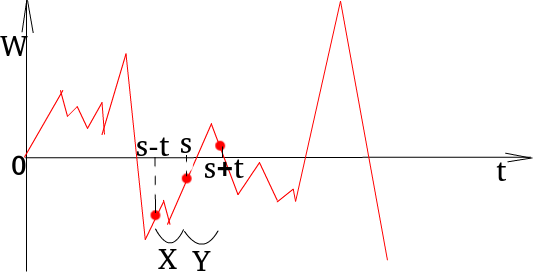
\includegraphics[width=.4\textwidth]{./pictures/5_6.png}
  \caption{График винеровского процесса}
  \label{fig:56}
\end{figure}

Есть 3 случайные величины.

У такого вектора есть плотность.
Случайные величины независимы
$$q_t =
  \iiint \limits_{x > y > z}
    p_{ \left( W \left( s \right), W \left( s - t \right), W \left( s + t \right) \right) }
      \left( x, y, z \right) dxdydz.$$

Вектор имеет нормальное распределение
$$ \begin{bmatrix}
    W \left( s \right) \\
    W \left( s - t \right) \\
    W \left( s + t \right)
  \end{bmatrix} \sim
  N \left(
    \left( \begin{bmatrix}
      0 \\
      0 \\
      0
    \end{bmatrix} \right),
    \left( \begin{bmatrix}
      s & s - t & s \\
      s - t & s - t & s - t \\
      s & s - t & s + t
    \end{bmatrix} \right) \right).$$

Нужно использовать какие-то свойства винеровского процесса.
Здесь нужно взять 2 приращения.
Эти приращения будут независимыми величинами с известным распределением $N \left( 0, t \right) $.

Вводим в рассмотрение приращения
$$ \begin{cases}
    X = W \left( s \right) - W \left( s - t \right), \\
    Y = W \left( s + t \right) - W \left( s \right).
  \end{cases}$$
Выразим из первого уравнения $W \left( s - t \right) = W \left( s \right) - X$,
а из второго --- $W \left( s + t \right) = W \left( s \right) + Y$.
Отнимем два последние уравнения
$$W \left( s + t \right) - W \left( s - t \right) =
  X + Y.$$
От всех частей неравенства в искомой вероятности вычтем $W \left( s - t \right) $
и заменим полученные выражения на введённые приращения
$$q_t =
  P \left\{
    W \left( s \right) - W \left( s - t \right) > 0 >
    W \left( s + t \right) - W \left( s - t \right) \right\} =
  P \left( X > 0 > X + Y \right).$$
Плотность вектора --- это произведение плотностей
$$P \left( X > 0 > X + Y \right) =
  \int \limits_{0}^{ \infty } \int \limits_{- \infty }^{-x}
    \frac{1}{2 \pi t} \cdot e^{-\frac{1}{2t} \left( x^2 + y^2 \right) } dydx =$$
Перейдём в полярную систему координат
$$x = r \cos \varphi, \,
  y = r \sin \varphi, \,
  dxdy = rdrd \varphi.$$
Получим
$$= \frac{1}{2 \pi t} \int \limits_0^{ \infty }
  \int \limits_{-\frac{ \pi }{2}}^{ \frac{ \pi }{4}} re^{-\frac{1}{2t} \cdot r^2} d \varphi dr =$$
Изобразим область интегрирования (рис. \ref{fig:561}).

\begin{figure}[h!]
  \centering
  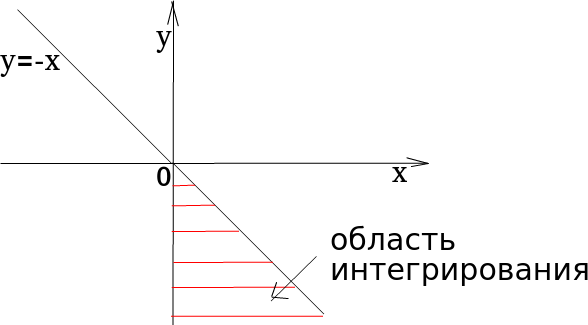
\includegraphics[width=.4\textwidth]{./pictures/5_6_1.png}
  \caption{Область интегрирования}
  \label{fig:561}
\end{figure}

По $ \varphi $ можем сразу проинтегрировать.
Интеграл по $ \varphi $ даст просто $ \frac{ \pi }{4}$.
Получаем
$$= \frac{1}{8} \int \limits_0^{ \infty } e^{-\frac{1}{2t} \cdot r^2} \cdot \frac{dr^2}{2t} =$$
Интеграл равен единице
$$= \frac{1}{8}$$

\subsubsection*{5.7}

\textit{Задание.}
Пусть $ \left\{ W \left( t \right), \, t \geq 0 \right\} $ --- винеровский процесс.
Найдите математическое ожидание и ковариационную функцию процессов:
\begin{enumerate}[label=\alph*)]
  \item $W^0 \left( t \right) = W \left( t \right) - tW \left( 1 \right), \, 0 \leq t \leq 1$
  (броуновский мост);
  \item $U \left( t \right) = e^{-\frac{t}{2}} W \left( e^t \right) $ (процесс Орнштейна-Уленбека).
\end{enumerate}
Выясните, какой из этих процессов является гауссовским.

\textit{Решение.}
\begin{enumerate}[label=\alph*)]
  \item $MW^0 \left( t \right) = 0$, потому что у винеровского процесса математическое ожидание 0.
  Найдём ковариационную функцию
  $$K \left( t, s \right) =
    cov \left[
      W \left( t \right) - tW \left( 1 \right), W \left( s \right) - sW \left( 1 \right) \right] =
    \min \left( t, s \right) - ts - st + st =$$
  Одинаковые слагаемые с разными знаками уничтожаются
  $$= \min \left( t, s \right) - st.$$

  Если возьмём вектор конечномерных распределений
  $$ \left( W^0 \left( t_1 \right), \dotsc, W^0 \left( t_n \right) \right),$$
  то этот вектор будет гауссовским.
  Такой процесс называется броуновский мост (рис. \ref{fig:57});

  \begin{figure}[h!]
    \centering
    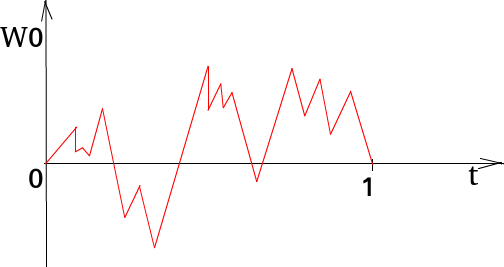
\includegraphics[width=.4\textwidth]{./pictures/5_7.png}
    \caption{Броуновский мост}
    \label{fig:57}
  \end{figure}

  \item $MU \left( t \right) = 0$, потому что винеровский.
  Ковариационная функция
  $$K \left( t, s \right) =
    cov \left[
      e^{-\frac{t}{2}} W \left( e^t \right), e^{-\frac{s}{2}} W \left( e^s \right) \right] =$$
  Выносим экспоненты (множители)
  $$= e^{-\frac{t}{2} - \frac{s}{2}} \min \left( e^t, e^s \right) =$$
  Экспонента --- монотонная функция
  $$= e^{-\frac{t}{2} - \frac{s}{2} + \min \left( t, s \right) } =
    e^{-\frac{1}{2} \left[ t + s - 2 \min \left( s, t \right) \right] } =
    e^{-\frac{1}{2} \cdot \left| t - s \right| }.$$
  Значение процесса $U \left( t \right) $ ---
  это линейное преобразование значений винеровского процесса, только в других точках.
  Процесс гауссовский.
\end{enumerate}

\subsubsection*{5.8}

\textit{Задание.}
Докажите, что случайный процесс
$$B \left( t \right) = \left( 1 - t \right) W \left( \frac{t}{1 - t} \right), \,
  0 \leq t < 1; \,
  B \left( 1 \right) = 0$$
имеет то же распределение, что и броуновский мост.

\textit{Решение.}
Конечномерные распределения такого процесса
$$ \left( B \left( t_1 \right), \dotsc, B \left( t_n \right) \right) $$
--- гауссовские вектора,
потому что это линейное преобразование винеровского процесса.

$MB \left( t \right) = 0$.

Найдём ковариацию
$$cov \left[ B \left( t \right), B \left( s \right) \right] =
  cov \left[
    \left( 1 - t \right) W \left( \frac{t}{1 - t} \right),
    \left( 1 - s \right) W \left( \frac{s}{1 - s} \right) \right] =$$
Множители выносим
$$= \left( 1 - t \right) \left( 1 - s \right)
  \min \left( \frac{t}{1 - t}, \frac{s}{1 - s} \right) =$$
Вносим положительный множитель в минимум
$$= \min \left( t - ts, s - ts \right) =$$
Общее выносим за минимум
$$= \min \left( t, s \right) - ts,$$
то есть ковариация такая же, как и у броуновского моста.

\addcontentsline{toc}{section}{Домашнее задание}
\section*{Домашнее задание}

\subsubsection*{5.12}

\textit{Задание.}
Пусть $ \left\{ W \left( t \right), \, t \geq 0 \right\} $ --- винеровский процесс.
Вычислите:
\begin{enumerate}[label=\alph*)]
  \item $M \left[
      \left( W \left( 4 \right) - 2W \left( 1 \right) + 2W \left( 2 \right) \right)^2 \right] $;
  \item $M \left[ \left( W \left( 1 \right) + 2W \left( 2 \right) + 1 \right)^3 \right] $;
  \item $M \left[ e^{W \left( 3 \right) - 2W \left( 2 \right) } \right] $;
  \item характеристическую функцию случайной величины $W \left( 1 \right) + 2W \left( 2 \right) + 1$.
\end{enumerate}

\textit{Решение.}
\begin{enumerate}[label=\alph*)]
  \item $W \left( 4 \right) - 2W \left( 1 \right) + W \left( 2 \right) =
    \xi \sim
    N \left( 0, 6 \right) $,
  потому что это линейная комбинация элементов гауссовского вектора.
  Найдём дисперссию
  $$D \xi =
    D \left[ W \left( 4 \right) - 2W \left( 1 \right) + W \left( 2 \right) \right] =
    cov \left( \xi, \xi \right) =$$
  Подставим выражения для случайной величины
  $$= cov \left[
      W \left( 4 \right) - 2W \left( 1 \right) + W \left( 2 \right),
      W \left( 4 \right) - 2W \left( 1 \right) + W \left( 2 \right) \right] =$$
  Воспользуемся линейностью
  \begin{gather*}
    = K \left( 4, 4 \right) - 2K \left( 4, 1 \right) + K \left( 4, 2 \right) -
    2K \left( 1, 4 \right) + 4K \left( 1, 1 \right) - 2K \left( 1, 2 \right) + \\
    + K \left( 2, 4 \right) - 2K \left( 2, 1 \right) + K \left( 2, 2 \right) = \\
    = 4 - 2 \cdot 1 + 2 - 2 \cdot 1 + 4 \cdot 1 - 2 \cdot 1 + 2 - 2 \cdot 1 + 2 =
    4 + 4 - 2 =
    6.
  \end{gather*}

  Нужно найти второй момент.
  $ \xi $ центрирована $M \xi^2 = D \xi = 6$;
  \item $W \left( 1 \right) + 2W \left( 2 \right) + 1 =
    \xi \sim
    N \left( 1, 5 \right) $,
  потому ято это линейная комбинация элементов гауссовского вектора.
  Найдём дисперсию.
  Константа на неё не влияет
  $D \xi =
    D \left[ W \left( 1 \right) - 2W \left( 2 \right) \right] =
    cov \left( \xi, \xi \right) $.
  Подставим выражения для случайной величины
  $$cov \left( \xi, \xi \right) =
    cov \left[
      W \left( 1 \right) + 2W \left( 2 \right) + 1,
      W \left( 1 \right) + 2W \left( 2 \right) + 1 \right] =$$
  Воспользуемся линейностью
  $$= \left( 1, 1 \right) + 2K \left( 1, 2 \right) + 2K \left( 2, 1 \right) +
    4K \left( 2, 2 \right) =
    1 + 2 + 2 + 8 =
    13.$$

  Нужно найти третий момент.
  $ \xi $ не центрирована.
  Нужно её центрировать $M \xi^3 = M \left[ \left( \xi - 1 \right) + 1 \right]^3$.
  Раскрываем скобки
  $$M \left[ \left( \xi - 1 \right) + 1 \right]^3 =
    M \left( \xi - 1 \right)^3 + 3M \left( \xi - 1 \right) + 3M \left( \xi - 1 \right) + 1 =$$
  По задаче 5.2 первое слагаемое --- 0, так как величина центрирована, второй момент --- 5,
  так как это дисперсия, первый момент --- ноль.
  Тогда
  $$= 0 + 3 \cdot 13 + 3 \cdot 0 + 1 = 38 + 1 = 40;$$
  \item $W \left( 3 \right) - 2W \left( 2 \right) = \xi \sim N \left( 0, 3 \right) $,
  потому что это линейная комбинация элементов гауссовского вектора.
  Найдём дисперсию
  $$D \xi =
    D \left[ W \left( 3 \right) - 2W \left( 2 \right) \right] =
    cov \left( \xi, \xi \right) =$$
  Подставим выражение для случайной величины
  $$= cov \left[
      W \left( 3 \right) - 2W \left( 2 \right), W \left( 3 \right) - 2W \left( 2 \right) \right] =$$
  Воспользуемся линейностью
  $$= K \left( 3, 3 \right) - 2K \left( 3, 2 \right) - 2K \left( 2, 3 \right) +
    4K \left( 2, 2 \right) =
    3 - 2 \cdot 2 - 2 \cdot 2 + 3 \cdot 2 =
    3.$$
  Нужно найти
  $$Me^{ \xi } =
    \int \limits_{ \mathbb{R}}
      \frac{1}{ \sqrt{6 \pi }} \cdot e^x \cdot p_{ \xi } \left( x \right) dx =
    \int \limits_{ \mathbb{R}}
      \frac{1}{6 \pi } \cdot e^x \cdot \frac{1}{6 \pi } \cdot e^{- \frac{x^2}{2 \cdot 9}} dx =
    \int \limits_{ \mathbb{R}} \frac{1}{ \sqrt{6 \pi }} \cdot e^{x - \frac{x^2}{18}} dx.$$
  Выделим полный квадрат в степени экспоненты
  $$ \frac{x^2}{18} - x =
    \frac{x^2}{ \left( 3 \sqrt{2} \right)^2} -
    2 \cdot \frac{1}{2} \cdot x \cdot \frac{1}{3 \sqrt{2}} \cdot 2 \sqrt{2} +
    \left( \frac{1}{2} \right)^2 \cdot \left( 2 \sqrt{2} \right)^2 =$$
  Три первых слагаемых образуют полный квадрат
  $$= \left( \frac{x}{3 \sqrt{2}} - \frac{3 \sqrt{2}}{2} \right)^2 + \frac{ 9 \cdot 2}{4} =
    \left( \frac{x}{3 \sqrt{2}} - \frac{3}{ \sqrt{2}} \right)^2 + \frac{9}{2} =
    \frac{ \left( x - 9 \right)^2}{2 \cdot 3} + \frac{9}{2}.$$
  Подставим полученное выражение в экспоненту
  $$ \int \limits_{ \mathbb{R}} \frac{1}{ \sqrt{6 \pi }} \cdot e^{x - \frac{x^2}{18}} dx =
    e^{- \frac{9}{2}}
    \int \limits_{ \mathbb{R}}
      \frac{1}{ \sqrt{6 \pi }} \cdot e^{- \frac{ \left( x - 9 \right)^2}{2 \cdot 9}} dx =$$
  Умножим и поделим на $ \sqrt{3}$ чтобы получить гауссовскую плотность
  $$= \sqrt{3} e^{- \frac{9}{2}}
    \int \limits_{ \mathbb{R}}
      \frac{1}{ \sqrt{2 \pi \cdot 9}} \cdot e^{-\frac{ \left( x - 9 \right)^2}{2 \cdot 9}} dx =$$
  Подинтергальная функция --- плотность нормального распределения,
  потому такой интеграл равен единице
  $$= \sqrt{3} e^{- \frac{9}{2}};$$
  \item нужно найти характеристическую функцию $W \left( 1 \right) + 2W \left( 2 \right) + 1$.

  Математическое ожидание такой величины равно 1, а дисперсия --- 13.
  Значит, получается
  $ \varphi_{W \left( 1 \right) =
    2W \left( 2 \right) + 1} \left( \lambda \right) =
    \varphi_{N \left( 1, 13 \right) } \left( \lambda \right) =
    e^{it - \frac{13t^2}{2}}$.
\end{enumerate}

\addcontentsline{toc}{chapter}{Занятие 6. Стохастическая непрерывность случайного процесса.
                                Существование непрерывной модификации}
\chapter*{Занятие 6. Стохастическая непрерывность случайного процесса.
          Существование непрерывной модификации}

\addcontentsline{toc}{section}{Контрольные вопросы и задания}
\section*{Контрольные вопросы и задания}

\subsubsection*{Приведите опредедение стохастически непрерывного процесса.}

Стохастически непрерывный процесс:
$ \xi \left( t \right) \overset{P} \xi \left( t_0 \right), \, t \to t_0$.

Это означает, что
$ \forall \varepsilon > 0 \qquad
  P \left( \left| \xi \left( t \right) - \xi \left( t_0 \right) \right| > \varepsilon \right) \to 0,
  \, t \to t_0$.

\subsubsection*{Сформулируйте достаточное условие существования непрерывной модификации случайного
                процесса.}

Пусть $ \xi \left( t \right), \, t \in \left[ 0, 1 \right] $ удовлетворяет условию
$$ \exists \alpha, \beta, C > 0: \qquad
  \forall t_1, t_2 \in \left[ 0, 1 \right] \qquad
  M \left| \xi \left( t_1 \right) =
  \xi \left( t_2 \right) \right|^{ \alpha } \leq C \left| t_1 - t_2 \right|^{1 + \beta }.$$
Тогда $ \xi $ имеет непрерывную модификацию.

\addcontentsline{toc}{section}{Аудиторные задачи}
\section*{Аудиторные задачи}

\subsubsection*{6.4}

\textit{Задание.}
Пусть $ \left\{ \xi \left( t \right), \, t \in \left[ 0, 1 \right] \right\} $ ---
случайный процесс, все значения которого являются независимыми и имеют одинаковое невырожденное
распределение.
Докажите, что этот процесс не является стохастически непрерывным ни в какой точке.

\textit{Решение.}
Распределения невырождены в том смысле, что это не константа (рис. \ref{fig:64}).

\begin{figure}[h!]
  \centering
  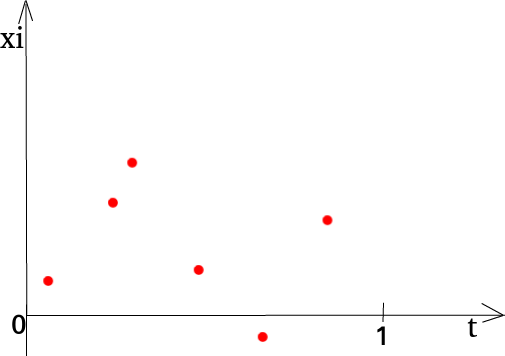
\includegraphics[width=.4\textwidth]{./pictures/6_4.png}
  \caption{График функции $ \xi \left( t \right) $}
  \label{fig:64}
\end{figure}

Стохастическая непрерывность означает, что вероятность
$$P \left\{ \left| \xi \left( s \right) - \xi \left( t \right) \right| > \varepsilon \right\} \to
  0.$$

Предположим, что распределение равномерное на отрезке $ \left[ 0, 1 \right] $.

Тогда такая вероятность равна
$$P \left\{ \left| \xi \left( s \right) - \xi \left( t \right) \right| > \varepsilon \right\} =
  \left( 1 - \varepsilon \right)^2 \not \to
  0, \,
  t \to s$$
(рис. \ref{fig:641}).

\begin{figure}[h!]
  \centering
  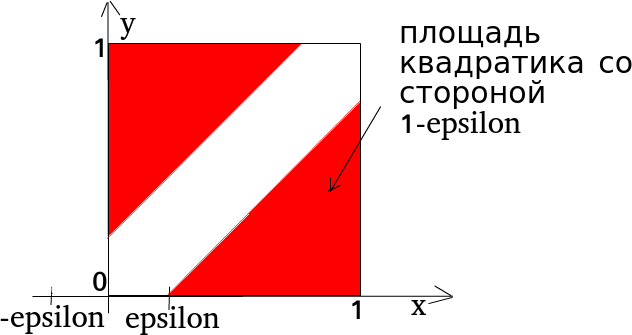
\includegraphics[width=.4\textwidth]{./pictures/6_4_1.png}
  \caption{Площадь квадратика со стороной $1 - \varepsilon$}
  \label{fig:641}
\end{figure}

Для такого процесса вероятность --- это постоянная и она не может стремиться к нулю.

\subsubsection*{6.5}

\textit{Задание.}
Пусть $X = \left\{ X \left( t \right), \, t \in T \right\} $ ---
стохастически непрерывный случайный процесс.
Докажите, что для произвольной непрерывной ограниченной функции $g$ функция
$M \left[ g \left( X \left( t \right) \right) \right] $ является непрерывной по $t$.

\textit{Решение.}
Нужно проверить, что если $t \to t_0$, то
$$M \left[ g \left( X \left( t \right) \right) \right] \to
  M \left[ g \left( X \left( t_0 \right) \right) \right].$$

Знаем, что если $t \to t_0$, то
$$X \left( t \right) \overset{P}{ \to }
  X \left( t_0 \right).$$
Следовательно, есть слабая сходимость.
Она как раз и означает, что такие математические ожидания должны сходиться.

\subsubsection*{6.6}

\textit{Задание.}
Пусть $ \left\{ X \left( t \right), \, t \in T \right\} $~---~стохастчески непрерывный процесс.
Докажите, что он является стохастически ограниченным, то есть:
$ \forall \varepsilon > 0 \, \exists C \, : \qquad \forall t \in \left[ a, b \right] \,
  P \left( \left| X \left( t \right) \right| > C \right) < \varepsilon $.

\textit{Решение.}
Непрерывная на отрезке функция ограничена.

Решим вспомогательную задачу,
то есть $f \, : \, \left[ a, b \right] \to \mathbb{R}$~---~непрерывная.

Тогда $f$~---~ограничена, то есть $sup \left| f \right| < \infty $.
Попробуем это доказать.

Предположим противное,
то есть $ \forall n \, \exists t_n \, : \, \left| f \left( t_n \right) \right| > n$.
Это бы означало неограниченность.

\subsubsection*{6.7}

\textit{Задание.}
Пусть $ \left\{ \xi \left( t \right), \, t \in \left[ a, b \right] \right\} $ ---
стохастически непрерывный процесс, а $f$ --- неслучайная функция,
определённая на $ \left[ a, b \right] $.
Докажите, что случайный процесс
$ \eta \left( t \right) =
  \xi \left( t \right) + f \left( t \right), \, t \in \left[ a, b \right] $
является стохастически непрерывным в тех и только тех точках отрезка $ \left[ a, b \right] $,
где является непрерывной функция $f$.

\textit{Решение.}
Нужно доказывать в обе стороны.

Сначала предположим, что $f$ --- непрерывная.
Пусть $f$ --- непрерывная в точке $t_0$.
Будем сейчас проверять, что сумма стохастически непрерывна.

Если $ \xi \left( t \right) $ --- стохастически непрерывна, то
$$ \xi \left( t \right) \overset{P}{ \to }
  \xi \left( t_0 \right)$$
при $t \to t_0$.

Сходимость по вероятности сохраняется при непрерывных операциях.
Сумма --- непрерывная операция.

Знаем, что $f$ --- непрерывна, то есть если $t \to t_0$,
то $f \left( t \right) \to f \left( t_0 \right) $.
От $ \omega $ тут зависимости нет.
Эту сходимость можно интерпретировать как сходимость почти наверное, следовательно,
$$f \left( t \right) \overset{P}{ \to }
  f \left( t_0 \right).$$

Значит и сумма будет сходиться.
Значит, отсюда следует, что $ \eta $ --- стохастически непрерывен.

Теперь предоложим, что вся сумма стохастически непрерывна.

Пусть $ \eta $ --- стохастически непрерывен в $t_0$.
Это значит, что
$$ \eta \left( t \right) \overset{P}{ \to } \eta \left( t_0 \right), \,
  t \to t_0.$$

Для $ \eta $ и $ \xi $ мы знаем, что есть сходимость по вероятности.
Надо взять разность.
Разность --- это $f$, то есть
$$ \begin{cases}
    \xi \left( t \right) + f \left( t \right) \overset{P}{ \to }
    \xi \left( t_0 \right) + f \left( t_0 \right), \\
    \xi \left( t \right) \overset{P}{ \to } \xi \left( t_0 \right).
  \end{cases}$$

Вычтем из первого второе
$$f \left( t \right) \overset{P}{ \to }
  f \left( t_0 \right).$$
Нужно проверить, что для неслучайной функции сходимость по вероятности и просто сходимость ---
одно и то же.
Сходимость по вероятности:
$ \forall \varepsilon > 0 \qquad
  P \left\{ \left| f \left( t \right) - f \left( t_0 \right) \right| > \varepsilon \right\} \to 0,
  \, t \to t_0$.
Это есть.
Просто сходимость: $ \forall \varepsilon > 0 \, \exists \delta > 0$,
чтобы выполнялось соотношение
$ \left| f \left( t \right) - f \left( t_0 \right) \right| <
  \varepsilon $
при $ \left| t - t_0 \right| < \delta $.
Это нужно проверить.

$ \forall \varepsilon > 0 \, \forall \alpha > 0 \, \exists \delta > 0 \qquad
  P \left\{ \left| f \left( t \right) - f \left( t_0 \right) \right| > \varepsilon \right\} <
  \alpha $
при $ \left| t - t_0 \right| < \delta $.

Функция $f$ --- неслучайная функция, то есть событие неслучайно.
Его вероятность равна или нулю, или единице.
Если $ \alpha > 1$, то вероятность равна нулю.
Значит, $ \left| f \left( t \right) - f \left( t_0 \right) \right| < \varepsilon $ при
$ \left| t - t_0 \right| <
  \delta $.
То есть $ \alpha < 1$.

Тогда
$P \left\{ \left| f \left( t \right) - f \left( t_0 \right) \right| > \varepsilon \right\} =
  0$.
Из этого следует, что при $ \left| t - t_0 \right| < \delta $ выполняется дополнение
$ \left| f \left( t \right) - f \left( t_0 \right) \right| \leq
  \varepsilon $.
Это и значит непрерывность в точке $t_0$.
Таким образом, для неслучайных величин все сходимости равносильны.

\subsubsection*{6.8}

\textit{Задание.}
Пусть $ \left\{ W \left( t \right), \, t \geq 0 \right\} $ --- винеровский процесс.
Докажите, что для произвольного $A > 0$
$$P \left\{
    \sum \limits_{i = 0}^{n - 1}
      \left| W \left( \frac{i + 1}{n} \right) - W \left( \frac{i}{n} \right) \right| > A
  \right\} \to
  1, \,
  n \to \infty.$$

\textit{Решение.}
Приращения --- нормальные независимые величины
$$W \left( \frac{i + 1}{n} \right) - W \left( \frac{i}{n} \right) \sim
  N \left( 0, \frac{1}{n} \right).$$

Сумма одинаково распределённых случайных величин
$$ \frac{1}{n} \sum \limits_{i = 1}^{n - 1}
    \left| W \left( \frac{i + 1}{n} \right) - W \left( \frac{1}{n} \right) \right| \cdot
  \sqrt{n} \overset{a.s.}{ \to }
  M \left| W \left( 1 \right) \right|, \,
  n \to \infty $$
по усиленному закону больших чисел, так как
$$ \sqrt{n} \left[ W \left( \frac{i + 1}{n} \right) - W \left( \frac{i}{n} \right) \right] \sim
  N \left( 0, 1 \right).$$

Тогда вероятность
$$P \left\{
    \sum \limits_{i = 0}^{n - 1}
      \left| W \left( \frac{i + 1}{n} \right) - W \left( \frac{i}{n} \right) \right| \cdot
    \frac{ \sqrt{n}}{n} \cdot \frac{n}{ \sqrt{n}} > A \right\} =
  P \left\{ M \left| W \left( 1 \right) \right| > 0 \right\} =
  1.$$

\subsubsection*{6.9}

\textit{Задание.}
Пусть $ \left\{ X \left( t \right), \, t \in T \right\} $ --- случайный процесс такой, что
$$MX \left( t \right) = 0, \,
  MX^2 \left( t \right) = 1$$
для произвольного $t \in T$.
\begin{enumerate}[label=\alph*)]
  \item Докажите, что $ \left| MX \left( t \right) X \left( t + h \right) \right| \leq 1$
  для произвольного $h > 0$ и произвольного $t \in \left[ 0, T - h \right] $.
  \item Допустим, что для некоторых $ \lambda < \infty, \, p > 1$ и $h_0 > 0$
  $$M \left[ X \left( t \right) X \left( t + h \right) \right] \geq
    1 - \lambda h^p$$
  для произвольного $h \in \left( 0, h_0 \right] $.
  Докажите, что $ \left\{ X \left( t \right), \, t \in T \right\} $ имеет непрерывную модификацию.
\end{enumerate}

\textit{Решение.}
\begin{enumerate}[label=\alph*)]
  \item Пусть $X \left( t \right) = \xi $ и $X \left( t + h \right) = \eta $.
  Тогда
  $$ \left| M \xi \eta \right| \leq
    M \left| \xi \eta \right| \leq
    \left( M \left| \xi \right|^p \right)^{ \frac{1}{p}}
    \left( M \left| \eta \right|^q \right)^{ \frac{1}{q}},$$
  где
  $$ \frac{1}{p} + \frac{1}{q} =
    1$$
  (неравенство Гёльдера).
  Возьмём $p = q = 2$.

  Получаем неравенство Коши-Буняковского
  $$M \left[ X \left( t \right) X \left( t + h \right) \right] \leq
    \left\{ M \left| X \left( t \right) \right|^2 \right\}^{ \frac{1}{2}}
    \left\{ M \left| X \left( t + h \right) \right|^2 \right\}^{ \frac{1}{2}} =
    1 \cdot 1 =
    1.$$
  \item Будем пользоваться достаточным условием Колмогорова
  $$ \exists \alpha, \beta, C > 0 \, : \,
    \forall t_1, t_2 \in \left[ 0, 1 \right] \qquad
    M \left| \xi \left( t_1 \right) - \xi \left( t_2 \right) \right|^{ \alpha } \leq
    C \left| t_1 - t_2 \right|^{1 - \beta }.$$
  Тогда у процесса будут непрерывные модификации.
  Нужно оценить
  $$M \left| X \left( t + h \right) - X \left( t \right) \right|^2 =
    M\left[X^2\left(t+h\right)-2X\left(t+h\right)X\left(t\right)+X^2\left(t\right)\right] =$$
  Воспользуемся линейностью математического ожидания
  $$= MX^2 \left( t + h \right) - 2M \left[  X \left( t + h \right) X \left( t \right) \right] +
    MX^2 \left( t \right).$$
  Здесь первое и последнее слагаемые равны единице, а второе не меньше $1 - \lambda h^p$.
  Тогда
  $$MX^2 \left( t + h \right) - 2M \left[  X \left( t + h \right) X \left( t \right) \right] +
    MX^2 \left( t \right) \geq
    2 - 2 \left( 1 - \lambda h^p \right) =
    2 \lambda h^p,$$
  где $2 \lambda = const, \, p = 1 + \beta $.

  Теорема Колмогорова работает с $ \alpha = 2, \, C = 2 \lambda $ и $ \beta = p - 1$.

  Значит, такой процесс имеет непрерывные модификации.
\end{enumerate}

\addcontentsline{toc}{section}{Домашнее задание}
\section*{Домашнее задание}

\subsubsection*{6.13}

\textit{Задание.}
На отрезке $ \left[ 0, 1 \right] $ независимым образом наугад выбраны две точки.
Пусть $ \xi \left( t \right) $ --- количество точек,
которые попали в интервал
$$ \left[ 0, t \right], \,
  t \in \left[ 0, 1 \right].$$
Найдите одномерные распределения процесса
$ \left\{ \xi \left( t \right), \, t \in \left[ 0, 1 \right] \right\} $.
Выясните, является ли этот процесс стохастически непрерывным.

\textit{Решение.}
Начнём с того, что найдём одномерные распределения.

$ \xi $ --- дискретная величина
$P \left\{ \xi \left( t \right) = k \right\} = C_2^k t^k \left( 1 - t \right)^{2 - k}, \,
  k \in \left\{ 0, 1, 2 \right\} $.

При $k = 0$ получаем
$P \left\{ \xi \left( t \right) = 0 \right\} =
  C_2^0 t^0 \left( 1 - t \right)^{2 - 0} =
  \left( 1 - t \right)^2$.

При $k = 1$ получаем
$P \left\{ \xi \left( t \right) = 1 \right\} =
  C_2^1 t^1 \left( 1 - t \right)^{2 - 1} =
  2t \left( 1 - t \right) $.

При $k = 2$ получаем
$P \left\{ \xi \left( t \right) = 2 \right\} =
  C_2^2 t^2 \left( 1 - t \right)^{2 - 2} =
  t^2$.

Будет ли этот процесс стохастически непрерывным?
Стохастическая непрерывность означает следующее
$P \left\{ \left| \xi \left( t \right) - \xi \left( s \right) \right| > \varepsilon \right\} \to
  0$,
когда $t \to s$ или $s \to t$.
Тогда
$P \left\{ \left| \xi \left( t \right) - \xi \left( s \right) \right| > \varepsilon \right\} =
  P$(в интервал $ \left[ s, t \right] $ попала хотя бы одна точка) $=
  P$(в интервал $ \left[ s, t \right] $ попала одна точка) $+
  P$(в интервал $ \left[ s, t \right] $ попало две точки) $=
  2 \left[ 1 - \left( t - s \right) \right] \left( t - s \right) + \left( t - s \right)^2 =
  2 \left( t - s \right) - \left( t - s \right)^2 \to
  0$,
когда $t \to s$ или $s \to t$.
То есть вывод такой, что этот процесс стохастически непрерывен.

\subsubsection*{6.14}

\textit{Задание.}
Пусть $ \left\{ W \left( t \right), \, t \geq 0 \right\} $ --- винеровский процесс.
Докажите, что
$$ \frac{W \left( t \right) }{t} \overset{P, \, n \to \infty }{ \to }
  0.$$

\textit{Решение.}
$$ \frac{W \left( t \right) }{t} \overset{P, \, n \to \infty }{ \to }
  0,$$
если
$$ \forall \varepsilon > 0 \,
  P \left\{ \left| \frac{W \left( t \right) }{t} \right| > \varepsilon \right\} \to 0,$$
когда $t \to \infty $.

Найдём математическое ожидание такой величины
$$M \frac{W \left( t \right) }{t} =
  \frac{1}{t} \cdot MW \left( t \right) =
  0.$$

Посчитаем дисперсию
$$D \frac{W \left( t \right) }{t} =
  \frac{1}{t^2} \cdot DW \left( t \right) =
  \frac{1}{t^2} \cdot t =
  \frac{1}{t}.$$

Используем неравенство Чебышева
\begin{gather*}
  P \left\{
    \left| \frac{W \left( t \right) }{t} - M \frac{W \left( t \right) }{t} \right| \geq \varepsilon
  \right\} =
  P \left\{ \left| \frac{W \left( t \right) }{t} - 0 \right| \geq \varepsilon \right\} \leq
  \frac{D \frac{W \left( t \right) }{t}}{ \varepsilon^2} =
  \frac{ \frac{1}{t}}{ \varepsilon^2} =
  \frac{1}{t \varepsilon^2} \to \\
  \to 0, \,
  t \to \infty.
\end{gather*}

\subsubsection*{6.15}

\textit{Задание.}
Докажите, что если случайный процесс $ \left\{ \xi \left( t \right), \, t \in \mathbb{R} \right\} $
имеет непрерывную функцию математического ожидания $m \left( t \right) $ и непрерывную по $t, s$
ковариационную функцию $K \left( t, s \right) $, то он является стохастически непрерывным.

\textit{Решение.}
Стохастическая непрерывность означает следующее
$$P \left\{ \left| \xi \left( t \right) - \xi \left( s \right) \right| > \varepsilon \right\} \to
  0,$$
когда $t \to s$ или $s \to t$.

Используем неравенство Чебышева
$$P \left\{
    \left|
      \xi \left( t \right) - \xi \left( s \right) -
      \left[ m \left( t \right) - m \left( s \right) \right] \right| \geq \varepsilon \right\} \leq
  \frac{D \left[ \xi \left( t \right) - \xi \left( s \right) \right] }{ \varepsilon^2} =$$
Дисперсия суммы нескольких случайных величин вычисляется по формуле
$$D \left( \xi_1, \dotsc, \xi_n \right) =
  \sum \limits_{i, j = 0}^n cov \left( \xi_i, \xi_j \right).$$
Тогда
$$= \frac{K \left( t, t \right) - K \left( t, s \right) - K \left( t, s \right) + K \left( s, s \right) }{ \varepsilon^2} \to
  0$$
при $t \to s$ или $s \to t$.
То есть вывод такой, что этот процесс стохастически непрерывен.

\subsubsection*{6.16}

\textit{Задание.}
Пусть $ \left\{ X \left( t \right), \, t \in T \right\} $~---~стохастически непрерывный процесс,
а $g$~---~непрерывная функция.
Докажите, что процесс $ \left\{ g \left( X \left( t \right) \right), \, t \in T \right\} $
тоже является стохастически непрерывным.

\textit{Решение.}
Процесс подставляется в функцию $g$.

Нужно проверить, что если $t \to s$, то
$P \left\{
    \left| g \left( X \left( t \right) \right) - g \left( X \left( s \right) \right) \right| >
    \varepsilon \right\}
  \to 0$.

Знаем, что если $t \to s$, то
\begin{equation*}
  X \left( t \right) \overset{P}{ \to }
  X \left( s \right),
\end{equation*}
функция $g$~---~непрерывная функция.
Тогда
\begin{equation*}
  g \left( X \left( t \right) \right) \overset{P}{ \to } g \left( X \left( s \right) \right), \,
  t \to s.
\end{equation*}
Непрерывная функция сохраняет сходимость по вероятности.

\subsubsection*{6.17}

\textit{Задание.}
Пусть все значения процесса $ \left\{ X \left( t \right), \, t \in \mathbb{R}^+ \right\} $
являются независимыми и равномерно распределёнными на $ \left[ 0, 1 \right] $.
Выясните, имеет ли этот процесс непрерывную модификацию.

\textit{Решение.}
Из задачи 6.4 $X \left( t \right) $ не стохастически непрерывен в каждой точке.

Стохастическая непрерывность означает,
что $X \left( t \right) \overset{P}{ \to } X \left( t_0 \right) $ при $t \to t_0$.

Пусть процесс $X \left( t \right) $ имеет непрерывную модификацию.
Тогда
$$ \begin{cases}
    X \left( t \right) = \tilde{X} \left( t \right) \, a.s., \\
    \tilde{X} \left( t \right) \to \tilde{X} \left( t_0 \right), \, t \to t_0, \\
    X \left( t_0 \right) = \hat{X} \left( t_0 \right) \, a.s.
  \end{cases} \Rightarrow X \left( t \right) \to X \left( t_0 \right) \, a.s.,$$
то есть процесс $X \left( t \right) $ стохастически непрерывен --- противоречие с условием.
Значит, $X \left( t \right) $ не имеет непрерывной модификации.

\subsubsection*{6.18}

\textit{Задание.}
Пусть $X = \left\{ X \left( t \right), \, t \in \mathbb{R}^+ \right\} $ ---
гауссовский процесс с нулевым математическим ожиданием и ковариационной функцией
$K \left( t, s \right) $, которая равна
\begin{enumerate}[label=\alph*)]
  \item $e^{-\left| t - s \right| }$,
  \item $ \left( t^{ \alpha } + s^{ \alpha } - \left| t - s \right|^{ \alpha } \right) / 2, \,
    \alpha \in \left( 0, 2 \right] $.
\end{enumerate}
Докажите, что $X$ имеет непрерывную модификацию.

\textit{Решение.}
Нам нужно доказать, что существуют такие константы
$$ \alpha > 0, \,
  \beta > 0, \,
  C > 0,$$
что
$M \left| X \left( t + h \right) - X \left( t \right) \right|^{ \alpha} \leq
  C \left| h \right|^{1 + \beta }$
для произвольных $t, \, t + h \in \mathbb{R}^+, \, h > 0$.

Поскольку процесс $X$ является гауссовским, то для произвольных
$$t, \, t + h \in \mathbb{R}^+$$
вектор $ \left( X \left( t \right), X \left( t + h \right) \right) $ является гауссовским.
Поэтому случайная величина $X \left( t + h \right) - X \left( t \right) $,
как линейная комбинация компонент гауссовского вектора, имеет нормальное распределение.
Найдём параметры этого распределения.
Имеем
$M \left[ X \left( t + h \right) - X \left( t \right) \right] =
  MX \left( t + h \right) - MX \left( t \right) =
  0$,
\begin{enumerate}[label=\alph*)]
  \item $D \left[ X \left( t + h \right) - X \left( t \right) \right] =
    M \left[ X \left( t + h \right) - X \left( t \right) \right]^2.$
  Раскроем квадрат
  $$M \left[ X \left( t + h \right) - X \left( t \right) \right]^2 =
    K \left( t + h, t + h \right) - 2K \left( t + h, t \right) + K \left( t, t \right) =$$
  Подставим выражения для ковариационной функции
  $$= e^{-\left| t + h - t - h \right| } - 2e^{-\left| t + h - t \right| } +
    e^{-\left| t - t \right| } =
    1 - 2e^{-\left| h \right| } + 1 =
    2 - 2e^{-h}.$$

  Тогда любой чётный момент случайной величины $X \left( t + h \right) - X \left( t \right) $ равен
  $M \left[ X \left( t + h \right) - X \left( t \right) \right]^{2n} =
    \left( 2n - 1 \right)!! \left( 2 - 2e^{-h} \right)^n$.

  Поскольку $1 - e^{-h} \leq h$ для $h > 0$,
  то $M \left[ X \left( t + h \right) - X \left( t \right) \right]^4 \leq 12h^2$ и, значит,
  достаточное условие Колмогорова существования непрерывной модификации выполняется при
  $ \alpha = 4, \,
    \beta = 1, \,
    C = 12$.
  \item Имеем
  $$D \left[ X \left( t + h \right) - X \left( t \right) \right] =
    M \left[ X \left( t + h \right) - X \left( t \right) \right]^2 =$$
  Раскроем квадрат
  \begin{gather*}
    = K \left( t + h, t + h \right) - 2K \left( t + h, t \right) + K \left( t, t \right) = \\
    = \frac{\left(t+h\right)^{\alpha}+\left(t+h\right)^{\alpha}-\left|t+h-t-h\right|^{\alpha}}{2}- \\
    - 2\cdot\frac{\left(t+h\right)^{\alpha}+t^{\alpha}-\left|t+h-t\right|^{\alpha}}{2} +
    \frac{t^{ \alpha } + t^{ \alpha } - \left| t - t \right|^{ \alpha }}{2} = \\
    = \left( t + h \right)^{ \alpha } - \left( t + h \right)^{ \alpha } - t^{ \alpha } -
    h^{ \alpha } + t^{ \alpha } =
    -h^{ \alpha }.
  \end{gather*}

  Тогда любой чётный момент случайной величины $X \left( t + h \right) - X \left( t \right) $ равен
  $M \left[ X \left( t + h \right) - X \left( t \right) \right]^{2n} =
    \left( 2n - 1 \right)!! \left( -h^{ \alpha } \right)^n$.

  В частности,
  $M \left[ X \left( t + h \right) - X \left( t \right) \right]^2 =
    3!! \left( -h^{ \alpha } \right) =
    3h^{ \alpha }$
  и, значит, достаточное условие Колмогорова существования непрерывной модификации выполняется при
  $ \alpha = 2, \,
    \beta = \alpha - 1 = 2 - 1 = 1, \,
    C = 3$.
\end{enumerate}

\subsubsection*{6.19}

\textit{Задание.}
Для процесса Пуассона найдите предел с вероятностью единица последовательности случайных величин
$$ \sum \limits_{i = 0}^{n - 1} \left( N \left( t_{i + 1} \right) - N \left( t_i \right) \right)^2$$
при $ \max \left( t_{i + 1} - t_i \right) \to 0$, где $0 = t_0 < t_1 < \dotsc < t_n = 1$ ---
разбитие отрезка $ \left[ 0, 1 \right] $.

\textit{Решение.}
$$P \left\{
    \sum \limits_{i = 0}^{n - 1} \left[ N \left( t_{i + 1} \right) - N \left( t_i \right) \right]^2 >
    \varepsilon \right\} \leq
  \frac{M\sum\limits_{i=0}^{n-1}\left[N\left(t_{i+1}\right)-N\left(t_i\right)\right]^2}{\varepsilon} =$$
Пользуемся независимостью приращений
$$=\frac{\sum\limits_{i=0}^{n-1}M\left[N\left(t_{i+1}\right)-N\left(t_i\right)\right]^2}{\varepsilon} =$$
Пользуемся однородностью приращений
$$= \frac{ \sum \limits_{i = 0}^{n - 1} MN^2 \left( t_{i + 1} - t_i \right) }{ \varepsilon } =
  \frac{1}{ \varepsilon }
  \sum \limits_{i = 0}^{n - 1}
    \left[ DN \left( t_{i + 1} - t_i \right) + M^2 N \left( t_{i + 1} - t_i \right) \right] =$$
Пусть случайная величина $X \left( t \right) $ с распределением Пуассона имеет параметр $ \lambda $.
Тогда
$$= \frac{1}{ \varepsilon }
  \sum \limits_{i = 0}^{n - 1} \left[
  \lambda \left( t_{i + 1} - t_i \right) + \lambda^2 \left( t_{i + 1} - t_i \right)^2 \right] =
  \frac{1}{ \varepsilon }
  \sum \limits_{i = 0}^{n - 1}
    \lambda \left( t_{i + 1} - t_i \right)
    \left[ 1 + \lambda \left( t_{i + 1} - t_i \right) \right] \leq$$
Оценим сумму максимумом
$$\leq \frac{n}{ \varepsilon } \cdot \left\{
    \lambda \max \left( t_{i + 1} - t_i \right)
    \left[ 1 + \lambda \max \left( t_{i + 1} - t_i \right) \right] \right\} \to
  0$$
при $ \max \left( t_{i + 1} - t_i \right) \to 0$, следовательно, предел по вероятности равен нулю.

\addcontentsline{toc}{chapter}{Занятие 7. $L_2$ теория}
\chapter*{Занятие 7. $L_2$ теория}

\addcontentsline{toc}{section}{Контрольные вопросы и задания}
\section*{Контрольные вопросы и задания}

\subsubsection*{Приведите опредедение непрерывного в среднем квадратическом случайного процесса.}

$ \xi $ непрерывен в среднем квадратическом в точке $t_0$, если
$$ \xi \left( t \right) \overset{L_2}{ \to }
  \xi \left( t_0 \right) $$
при $t \to t_0$,
то есть $M \left[ \xi \left( t \right) - \xi \left( t_0 \right) \right]^2 \to 0, \, t \to t_0$.

Случайный процесс $ \xi $ непрерывен в среднем квадратическом на $T$,
если $ \xi $ непрерывен в среднем квадратическом в каждой точке $t_0 \in T$.

\subsubsection*{Как определяются производная случайного процесса, интеграл случайного процесса?}

$ \xi $ дифференцируем в среднем квадратическом в точке $t_0$, если
$$ \exists L_2-\lim \limits_{t \to t_0}
    \frac{ \xi \left(t \right) - \xi \left( t_0 \right) }{t - t_0} =
  \xi' \left( t_0 \right).$$

Случайный процесс $ \xi $ интегрируем в среднем квадратическом на отрезке $ \left[ a, b \right] $,
если
$$ \exists L_2-\lim \limits_{ \left| \pi \right| \to 0}
    \sum \limits_{k = 0}^{n - 1} \xi \left( t_k \right) \Delta t_k,$$
где $ \pi $ --- разбиение: $a = t_0 < \dotsc < t_n = b$.

Модуль разбиения --- это максимумальная разность между соседними точками.

\subsubsection*{Как изменяются характеристики случайного процесса при дифференцировании,
                интегрировании?}

$ \xi \in L_2 \, : \, M \left| \xi \right|^2 < \infty, \,
  \left( \xi, \eta \right) = M \xi \overline{ \eta }, \,
  \left( \xi, \xi \right) = M \left| \xi \right|^2$.

\subsubsection*{Приведите условия непрерывности, дифференцируемости,
                интегрируемости случайного процесса в терминах его ковариационной функции.}

$ \xi $ непрерывен в среднем квадратическом на интервале $T$ тогда и только тогда,
когда $m \in C \left( T \right), \, K \in C \left( T \times T \right) $.

Случайный процесс $ \xi $ дифференцируем в среднем квадратическои в точке $t_0$
тогда и только тогда, когда $m$ дифференцируема в точке $t_0$ и
$$ \exists \lim \limits_{s, t \to t_0}
    \frac{K \left( t, s \right) - K \left( t, t_0 \right) - K \left( t_0, s \right) + K \left( t_0, t_0 \right) }{ \left( s - t_0 \right) \left( t - t_0 \right) }.$$

Непрерывный в среднем квадратическом на отрезке $ \left[ a, b \right] $ процесс $ \xi $
интегрируем в среднем квадратическом на этом отрезке.

\addcontentsline{toc}{section}{Аудиторные задачи}
\section*{Аудиторные задачи}

\subsubsection*{7.2}

\textit{Задание.}
Пусть $ \zeta_1, \dotsc, \zeta_n$ --- интегрируемые с квадратом случайные величины.
Докажите, что случайный процесс
$$ \xi \left( t \right) =
  \sum \limits_{k = 1}^n \zeta_k e^{kt}$$
имеет производную в среднем квадратическом и найдите её.

\textit{Решение.}
$ \zeta_1, \dotsc, \zeta_n \in L_2$, то есть есть $n$ величин, и процесс определяется как
$$ \xi \left( t \right) =
  \sum \limits_{k = 1}^n \zeta_l e^{kt}.$$
Нужно проверить, что этот процесс дифференцируем и найти его производную в $L_2$.

Время $t$ входит только в экспоненту, которую мы умеем дифференцировать.
Нужно проверить, что
$$ \left \Vert
    \frac{ \xi \left( t \right) - \xi \left( t_0 \right) }{t - t_0} -
    \sum \limits_{k = 1}^n \zeta_k ke^{kt_0} \right \Vert \to
  0,$$
когда $t \to t_0$.

Будем это проверять.
Можно $ \xi \left( t \right) $ расписать.

$ \xi \left( t \right) $ --- это сумма
$$ \left \Vert
    \frac{ \xi \left( t \right) - \xi \left( t_0 \right) }{t - t_0} -
    \sum \limits_{k = 1}^n \zeta_k k e^{kt_0} \right \Vert =
  \left \Vert
    \frac{ \sum \limits_{k = 1}^n \zeta_k e^{kt} - \sum \limits_{k = 1}^n \zeta_k e^{kt_0}}{t - t_0} -
    \sum \limits_{k = 1}^n \zeta_k ke^{kt_0} \right \Vert =$$
Во всех слагаемых есть сумма и $ \zeta_k$.
Так что приведём подобные, и будет одна сумма
$$= \left \Vert
    \sum \limits_{k = 1}^n \zeta_k \left( \frac{e^{kt} - e^{kt_0}}{t - t_0} - ke^{kt_0} \right)
  \right \Vert \leq$$
Первое слагаемое в скобках стремится к производной, а второе и есть производная.
Из разность стремится к нулю.
Используем неравенство треугольника
$$ \leq \sum \limits_{k = 1}^n
  \left \Vert \zeta_k \left( \frac{e^{kt} - e^{kt_0}}{t - t_0} - ke^{kt_0} \right) \right \Vert =$$
С помощью свойства
$ \left \Vert \alpha \xi \right \Vert \leq
  \left| \alpha \right| \cdot \left \Vert \xi \right \Vert $
коэффициент выносится из нормы
$$= \sum \limits_{k = 1}^n
    \left| \frac{e^{kt} - e^{kt_0}}{t - t_0} - ke^{kt_0} \right| \cdot
    \left \Vert \zeta_k \right \Vert \to$$
Под модулем стоят числа, которые сходятся к нулю, под нормой --- числа
$$ \to 0.$$

\subsubsection*{7.3}

\textit{Задание.}
Пусть $ \left\{ W \left( t \right), \, t \geq 0 \right\} $ --- винеровский процесс.
Докажите, что случайный процесс
$$ \left\{ \eta \left( t \right) = \int \limits_0^t W \left( s \right) ds, \, t \geq 0 \right\} $$
являюется дифференцируемым в среднем квадратическом и что
$$ \eta' \left( t \right) =
  W \left( t \right) $$
для произвольного $t \geq 0$.

\textit{Решение.}
Дифференцируем интеграл по верхнему пределу.

Должна получиться подинтегральная функция.
Нужно проверить, что
$$ \frac{ \eta \left( t \right) - \eta \left( t_0 \right) }{t - t_0} \overset{L_2}{ \to }
  W \left( t_) \right).$$

Проверяем.
Вместо $ \eta $ подставляем интеграл
$$M \left[
    \frac{ \eta \left( t \right) - \eta \left( t_0 \right) }{t - t_0} - W \left( t_0 \right)
  \right]^2 =
  M \left[
    \frac{ \int \limits_0^t W \left( s \right) ds - \int \limits_0^{t_0} W \left( s \right) ds}{t - t_0} -
    W \left( t_0 \right)
  \right]^2 =$$
Разность интегралов --- это интеграл от $t_0$ до $t$.
Так что
$$= M \left[
    \frac{\int \limits_{t_0}^t W \left( s \right) ds}{t - t_0} - W \left( t_0 \right)
  \right]^2 =$$
Случайную величину $W \left( t_0 \right) $ можно внести под интеграл,
потому что он не зависит от $s$.
Знаменатель вынесем из-под интеграла
$$= M \left\{
    \int \limits_{t_0}^t \left[
      W \left( s \right) - W \left( t_0 \right)
    \right] ds
  \right\}^2 \cdot
  \frac{1}{ \left( t - t_0 \right)^2} =$$
Найдём дисперсию
$$D \int \limits_a^b \xi \left( s \right) ds =
  cov \left(
    \int \limits_a^b \xi \left( s \right) ds, \int \limits_a^b \xi \left( r \right) dr
  \right).$$
Ковариация --- это линейная функция, оба интеграла выносятся
$$cov \left(
    \int \limits_a^b \xi \left( s \right) ds, \int \limits_a^b \xi \left( r \right) dr
  \right) =
  \int \limits_a^b \int \limits_a^b
    cov \left[ \xi \left( s \right), \xi \left( t \right) \right]
  dsdr.$$
Тогда
$$= \frac{1}{ \left( t - t_0 \right)^2} \int \limits_{t_0}^t \int \limits_{t_0}^t cov \left[
    W \left( s \right) - W \left( t_0 \right), W \left( r \right) - W \left( t_0 \right) \right]
  dsdr =$$
Ковариацию винеровского процесса мы знаем
$$= \int \limits_{t_0}^t \int \limits_{t_0}^t \left[
    \min \left( s, r \right) - t_0 - t_0 + t_0 \right] dsdr \cdot
  \frac{1}{ \left( t - t_0 \right)^2} =$$
Одинаковые слагаемые с разными знаками уничножаются
$$= \int \limits_{t_0}^t \int \limits_{t_0}^t
    \left[ \min \left( s, r \right) - t_0 \right] dsdr \cdot
  \frac{1}{ \left( t - t_0 \right)^2} \leq
  \int \limits_{t_0}^t \int \limits_{t_0}^t \left( t - t_0 \right) dsdr \cdot
  \frac{1}{ \left( t - t_0 \right)^2} =$$
Величина $t - t_0 = const$, она вносится
$$= t - t_0 \to
  0.$$
Это и надо было проверить.

\subsubsection*{7.4}

\textit{Задание.}
Пусть $ \left\{ W \left( t \right), \, t \geq 0 \right\} $ --- винеровский процесс.
Докажите существование интеграла в среднем квадратическом
$$ \int \limits_0^{ \infty } e^{-t} W \left( t \right) dt =
  L_2-\lim \limits_{T \to + \infty } \int \limits_0^T e^{-t} W \left( t \right) dt$$
и найдите его распределение.

\textit{Решение.}
Рассматриваются интегралы
$$ \int \limits_0^T e^{-t} W \left( t \right) dt.$$
Нужно доказать, что у этих интегралов есть предел, то есть
$$ \int \limits_0^T e^{-t} W \left( t \right) dt \overset{L_2, \, T \to \infty }{ \to }?$$

Что нужно проверять, чтобы доказать, что этот интеграл сходится?
Надо брать математическое ожидание разностей в квадрате.
Предела мы не знаем.

Гильбертово пространство обладает свойством полноты
$$ \xi_n \overset{L_2, \, n \to \infty }{ \to }
  \xi$$
тогда и только тогда, когда $ \left\{ \xi_n \right\} $ фундаментальная, то есть
$$M \left( \xi_n - \xi_m \right)^3 \overset{n, m \to \infty }{ \to }
  0.$$

Предположим, что $T_1 < T_2$.
Из полноты следует, что нам достаточно проверить такое
$$M \left[
    \int \limits_0^{T_1} e^{-t} W \left( t \right) dt -
    \int \limits_0^{T_2} e^{-t} W \left( t \right) dt \right]^2 =
  M \left[ \int \limits_{T_1}^{T_2} e^{-t} W \left( t \right) dt \right]^2 =$$
Это двойной интеграл от ковариации
$$= \int \limits_{T_1}^{T_2} \int \limits_{T_1}^{T_2}
    cov \left[ e^{-t} W \left( t \right), e^{-s} W \left( s \right) \right] dtds =
  \int \limits_{T_1}^{T_2} \int \limits_{T_1}^{T_2}
    e^{-t-s} \min \left( t, s \right) dtds =$$
Нужно проверить, что это выражение стремится к нулю, когда $T_1, T_2 \to \infty $.
Распишем для всех случаев
$$= \int \limits_{T_1}^{T_2} \left( \int \limits_{T_1}^s e^{-t-s} tdt \right) ds +
  \int \limits_{T_1}^{T_2} \left( \int \limits_s^{T_2} e^{-t-s} sdt \right) ds \leq $$
Пусть $t < s$.
Тогда
$$ \leq \int \limits_{T_1}^{T_2} \left( \int \limits_{T_1}^s e^{-t-s} sdt \right) ds +
  \int \limits_{T_1}^{T_2} \left( \int \limits_s^{T_2} e^{-t-s} sdt \right) ds =
  \int \limits_{T_1}^{T_2} \int \limits_{T_1}^{T_2} e^{-s} e^{-t} sdtds =$$
Интегрируем по $y$, получаем
$$= \int \limits_{T_1}^{T_2} se^{-s} ds \int \limits_{T_1}^{T_2} e^{-t} dt =
  \int \limits_{T_1}^{T_2} se^{-s} ds \cdot \left( e^{-T_2} - e^{-T_1} \right) =$$
Берём интеграл по частям
$$= \left( e^{-T_2} - e^{-T_1} \right)
  \left( \left. -e^{-s} s \right|_{T_1}^{T_2} - \left. e^{-s} \right|_{T1}^{T_2} \right) =$$
Подставим пределы интегрирования
$$= \left( e^{-T_2} - e^{-T_1} \right)
  \left( -T_2 e^{-T_2} + T_1 e^{-T_1} - e^{-T_2} + e^{-T_1} \right)
  \overset{T_1, T_2 \to \infty }{ \to } 0,$$
Так как каждое слагаемое стремится к нулю,
то есть мы посчитали расстояние между двумя интегралами и показали, что оно стремится к нулю
$$ \exists \lim \limits_{T \to \infty } \int \limits_0^T e^{-t} W \left( t \right) dt =
  \int \limits_0^{ \infty } e^{-t} W \left( t \right) dt.$$

Теперь скажем, какое распределение у этого предела.

$W$ --- это винеровский процесс, а интеграл --- это предельные суммы, так что
$$ \int \limits_0^T e^{-t} W \left( t \right) dt \sim
  N \left( 0, \int \limits_0^T \int \limits_0^T e^{-t-s} \min \left( t, s \right) dtds \right).$$

Предел гауссовской величины --- это тоже нормальная величина
$$ \int \limits_0^{ \infty } e^{-t} W \left( t \right) dt \sim
  N \left(
    0, \int \limits_0^{ \infty } \int \limits_0^{ \infty } e^{-t-s} \min \left( t, s \right) dtds
  \right).$$

\addcontentsline{toc}{chapter}{Занятие 8. Стационарные случайные процессы}
\chapter*{Занятие 8. Стационарные случайные процессы}

\addcontentsline{toc}{section}{Контрольные вопросы и задания}
\section*{Контрольные вопросы и задания}

\subsubsection*{Приведите определение случайного процесса, стационарного в широком смысле.}

$ \xi \left( t \right), \, t \in T$ называется стационарным в широком смысле (стационарным), если
\begin{enumerate}
  \item $m \left( t \right) \equiv m \, \left( const \right) $;
  \item $K \left( t, s \right) = K \left( t + r, s + r \right), \, \forall t, s, r \in T$.
  Это означает, что ковариационная функция --- это сейчас функция разности аргументов,
  то есть $K \left( t, s \right) = k \left( t - s \right) $.
\end{enumerate}

\subsubsection*{Приведите определение ковариационной функции случайного процесса.}

$K \left( t, s \right) =
  M \left[ \xi \left( t \right) - m \left( t \right) \right] \cdot
  \left[ \xi \left( s \right) - m \left( s \right) \right], \,
  t, s \in T$.

\subsubsection*{Сформулируйте теорему Бохнера про спектральное изображения ковариационной функции
                стационарного в широком смысле случайного процесса.}

Пусть $ \xi \left( t \right), \, t \in \mathbb{R}$ ---
это стационарный и непрерывный в среднем квадратическом случайный процесс.
Тогда существует конечная мера $ \mu $ на $ \mathbb{R}$ такая, что
$$k \left( t \right) =
  \int \limits_{-\infty}^{+\infty} e^{it \lambda } \mu \left( d \lambda \right),$$
мера $ \mu $ определяется единственным образом.

\subsubsection*{Что называется спектральной функцией, спектральной плотностью стационарного в
                широком смысле случайного процесса?}

$ \mu $ называеься спектральной мерой, а если есть плотность $p$, то $p$ ---
это спектральная плотность.

\addcontentsline{toc}{section}{Аудиторные задачи}
\section*{Аудиторные задачи}

\subsubsection*{8.2}

\textit{Задание.}
Пусть $A, \eta, \varphi $ --- независимые случайные величины,
причём $ \varphi $ имеет равномерное распределение на отрезке $ \left[ 0, 2 \pi \right] $.
Докажите, что процесс
$ \left\{
    \xi \left( t \right) = A \cos \left( t \eta + \varphi \right), \, t \in \mathbb{R}
  \right\} $
является стационарным в широком смысле.

\textit{Решение.}
$$M \xi \left( t \right) =
  M \left[ A \cos \left( \eta t + \varphi \right) \right] =
  MA \cdot M \cos \left( \eta t + \varphi \right) =$$
Распишем косинус суммы
$$= MA \cdot M \left[
    \cos \left( \eta t \right) \cos \varphi - \sin \left( \eta t \right) \sin \varphi \right] =$$
Все множители независимы
$$= MA \cdot M \cos \left( \eta t \right) \cdot M \cos \varphi -
  MA \cdot M \sin \left( \eta t \right) \cdot M \sin \varphi =$$
Сгруппируем множители
$$= M \left[ A \cos \left( \eta t \right) \right] \cdot M \cos \varphi -
  M \left[ A \sin \left( \eta t \right) \right] \cdot M \sin \varphi =$$
Запишем математическое ожидание $ \sin \varphi $
через интеграл от плотности равномерного распределения
$$= M \left[ A \cos \left( \eta t \right) \right]
  \int \limits_{ \mathbb{R}} \cos x \cdot p \left( x \right) dx -
  M \left[ A \sin \left( \eta t \right) \right]
  \int \limits_{ \mathbb{R}} \sin x \cdot p \left( x \right) dx =$$
Подставим плотность
$$= M \left[ A \cos \left( \eta t \right) \right] \int \limits_0^{2 \pi } \cos xdx -
  M \left[ A \sin \left( \eta t \right) \right] \int \limits_0^{2 \pi } \sin xdx =$$
Возьмём интегралы
$$= M \left[ A \cos \left( \eta t \right) \right] \cdot \left. \sin x \right|_0^{2 \pi } -
  M \left[ A \sin \left( \eta t \right) \right] \cdot
  \left. \left( - \cos x \right) \right|_0^{2 \pi } =
  0.$$

Ковариационная функция
$$K \left( t, s \right) =
  M \xi \left( t \right) \xi \left( s \right) =
  M A^2 \cdot M \cos \left( \eta t + \varphi \right) \cdot \cos \left( \eta s + \varphi \right) =$$
Распишем произведение косинусов
$$= \frac{MA^2}{2} \cdot \left\{
  M \cos \left[ \eta \left( t + s \right) + 2 \varphi \right] +
  M \cos \left[ \eta \left( t - s \right) \right] \right\} =$$
Первое слагаемое равно нулю
$$= \frac{MA^2}{2} \cdot M \cos \left[ \eta \left( t - s \right) \right].$$
Значит, процесс стационарный.

\subsubsection*{8.3}

\textit{Задание.}
Пусть $ \left\{ N \left( t \right), \, t \geq 0 \right\} $ ---
процесс Пуассона с параметром $ \lambda $.
Докажите, что процесс
$ \left\{ \xi \left( t \right) = N \left( t + 1 \right) - N \left( t \right), \, t \geq 1 \right\} $
является стационарным в широком смысле.

\textit{Решение.}
$ \left\{ \xi \left( t \right) = N \left( t + 1 \right) - N \left( t \right), \, t \geq 1 \right\} $
--- процесс приращений пуассоновского процесса.

\begin{enumerate}
  \item
  $$M \xi \left( t \right) =
    M \left[ N \left( t + 1 \right) - N \left( t \right) \right] =
    MN \left( t + 1 \right) - MN \left( t \right) =
    \lambda \left( t + 1 \right) - \lambda t =
    \lambda,$$
  то есть математическое ожидание постоянное.
  \item Теперь найдём ковариационную функцию
  $$K \left( t, s \right) =
    cov \left[ \xi \left( t \right), \xi \left( s \right) \right] =
    cov \left[
      N \left( t + 1 \right) - N \left( t \right),
      N \left( s + 1 \right) - N \left( s \right) \right] =$$
  Известно, что
  $cov \left[ N \left( t \right), N \left( s \right) \right] =
    \lambda \min \left( t, s \right) $.
  Раскрываем ковариацию и получаем 4 слагаемых
  $$= \lambda \left[
      \min \left( t + 1, s + 1 \right) - \min \left( t + 1, s \right) -
      \min \left( t, s + 1 \right) + \min \left( t, s \right) \right] =$$
  Возможные случаи изображены на рисунке \ref{fig:83}.

  \begin{figure}[h!]
    \centering
    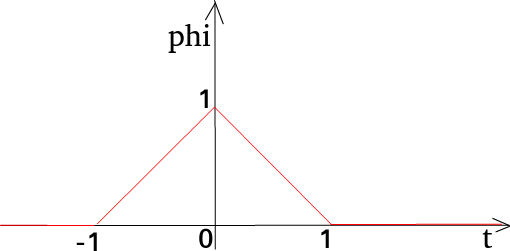
\includegraphics[width=.4\textwidth]{./pictures/4_2.png}
    \caption{Возможные случаи (два последних симметричны двум первым)}
    \label{fig:83}
  \end{figure}

  В первом случае
  $$= 0.$$
  Во втором случае
  $$= \lambda \left[ s + 1 - t \right].$$

  Запишем ковариационную функцию
  $$K \left( t, s \right) =
    \begin{cases}
      0, \qquad s + 1 \leq t \, \left( 1 \leq t - s \right), \\
      \lambda \left[ 1 - \left( t - s \right) \right],
      \qquad s \leq t \leq s + 1 \, \left( 0 \leq t - s \leq 1 \right), \\
      0, \qquad s \geq t + 1 \, \left( t - s \leq 1 \right), \\
      \lambda \left[ 1 - \left( s - t \right) \right],
      \qquad t \leq s \leq t + 1 \, \left( -1 \leq t - s \leq 0 \right).
    \end{cases}$$

  Надо понять, это функция от разности или нет.
  Условия переписываются через разности, тогда ковариация зависит от разности.

  Сейчас
  $$K \left( t, s \right) =
    \begin{cases}
      0, \qquad \left| t - s \right| \geq 1, \\
      \lambda \left( 1 - \left| t - s \right| \right), \qquad \left| t - s \right| \leq 1.
    \end{cases}$$
\end{enumerate}

\subsubsection*{8.4}

\textit{Задание.}
Пусть $ \left\{ W \left( t \right), \, t \geq 0 \right\} $ --- винеровский процесс.
Надите сектральную функцию процесса
$ \left\{
  \xi \left( t \right) = W \left( t + 1 \right) - W \left( t \right), \, t \geq 0 \right\} $.

\textit{Решение.}
Если $ \left\{ \xi_n, \, n \in \mathbb{Z} \right\} $ ---
это стационарная последовательность с $K \left( n, m \right) = k \left( n - m \right) $,
тогда теорема Герглотца говорит,
что функцию $k$ можно представить как преобразование Фурье какой-то меры, то есть
$$k \left( n \right) =
  \frac{1}{2 \pi } \int \limits_{-\pi }^{ \pi } e^{i \lambda n} \mu \left( d \lambda \right).$$

Эта мера называется спектральной мерой.

Это в слуае дискретного времени.
Для непрерывного времени если
$$ \left\{ \xi \left( t \right), \, t \in \mathbb{R} \right\} $$~---~это стационарный процесс,
непрерывный в $L_2$, его ковариационная функция ---
это $K \left( t, s \right) = k \left( t - s \right) $, в этом случае есть теорема Бохнера,
которая говорит, что
$$k \left( t \right) =
  \frac{1}{2 \pi }
  \int \limits_{-\infty }^{+\infty } e^{i \lambda t} \mu \left( d \lambda \right).$$

Если у этой меры есть плотность, то она называется спектральной плотностью.

$$K \left( t, s \right) =
  \begin{cases}
    1 - \left| t - s \right|, \, \left| t - s \right| \leq 1, \\
    0, \qquad \left| t - s \right| \geq 1.
  \end{cases}$$

Это то же самое, что
$$k \left( t \right) =
  \begin{cases}
    1 - \left| t \right|, \qquad \left| t \right| \leq 1, \\
    0, \qquad \left| t \right| \geq 1.
  \end{cases}$$

Теперь нужно подобрать меру, для которой это --- преобразование Фурье.

Сейчас спектральная плотность
$$p \left( \lambda \right) =
  \int \limits_{-\infty }^{+\infty } k \left( t \right) e^{-i \lambda t} dt =
  \int \limits_{-1}^1 \left( 1 - \left| t \right| \right) e^{-i \lambda t} dt =$$
Экспонента расписывается по формуле Эйлера как сумма косинуса и синуса,
умноженного на мнимую единицу.
Интеграл от синуса равен нулю, так как синус --- нечётная функция, $1 - \left| t \right| $ ---
чётная функция, интегрирование происходит по симметричному отрезку
$$= 2 \int \limits_0^1 \left( 1 - t \right) \cos \lambda t dt =$$
Интегрируем по частям, при этом $1 - \left| t \right| = u$, а $ \cos \lambda t = v$.
Тогда
$$= 2 \left. \left( 1 + t \right) \cdot \frac{ \sin \lambda t}{ \lambda } \right|_0^1 +
  \frac{2}{ \lambda } \int \limits_0^1 \sin \lambda t dt =$$
Первое слагаемое равно нулю
$$= \frac{2}{ \lambda^2} \left( 1 - \cos \lambda \right).$$

\addcontentsline{toc}{section}{Домашнее задание}
\section*{Домашнее задание}

\subsubsection*{8.10}

\textit{Задание.}
Докажите, что сумма независимых стационарных в широком смысле процессов является стационарным в
широком смысле процессом.

\textit{Решение.}
Пусть $ \left\{ \xi_i \left( t \right), \, t \in T \right\}, \, i = \overline{1, n}$ ---
независимые стационарные в широком смысле процессы.
Нужно доказать, что процесс
$$ \left\{
  \eta \left( t \right) = \sum \limits_{i = 1}^n \xi_i \left( t \right), \, t \in T \right\} $$
является стационарным в широком смысле.

$$M \eta \left( t \right) =
  M \sum \limits_{i = 1}^n \xi_i \left( t \right) =
  \sum \limits_{i = 1}^n M \xi_i \left( t \right) =
  \sum \limits_{i = 1}^n m_i =
  m =
  const.$$

Ковариационная функция
$$K \left( t, s \right) =
  cov \left[ \eta \left( t \right), \eta \left( s \right) \right] =
  cov \left[
    \sum \limits_{i = 1}^n \xi_i \left( t \right), \sum \limits_{j = 1}^n \xi_j \left( s \right)
  \right] =$$
Вынесем суммы, так как ковариация --- линейная функция
$$= \sum \limits_{i = 1}^n
    \sum \limits_{j = 1}^n cov \left[ \xi_i \left( t \right), \xi_j \left( s \right) \right] =
  \sum \limits_{i = 1}^n cov \left[ \xi_i \left( t \right), \xi_i \left( s \right) \right] =
  \sum \limits_{i = 1}^n K_i \left( t, s \right) =$$
Все $ \xi_i \left( t \right) $ стационарные,
поэтому их ковариационные функции зависят только от разности аргументов
$$= \sum \limits_{i = 1}^n k_i \left( t - s \right) =
  k \left( t - s \right).$$
Значит, процесс стационарный.

\subsubsection*{8.11}

\textit{Задание.}
Пусть $ \xi_1, \xi_2$ --- независимые одинаково распределённые случайные величины,
которые принимают значения $+1$ и $-1$ с вероятностью $1 / 2$.
Докажите, что процесс
$ \left\{
  \xi \left( t \right) = \xi_1 \cos \lambda t + \xi_2 \sin \lambda t, \, t \in \mathbb{R} \right\} $
является стационарным в широком смысле.

\textit{Решение.}
$$M \xi \left( t \right) =
  M \left( \xi_1 \cos \lambda t + \xi_2 \sin \lambda t \right) =
  M \left( \xi_1 \cos \lambda t \right) + M \left( \xi_2 \sin \lambda t \right) =$$
Вынесем константы
$$= \cos \lambda t \cdot M \xi_1 + \sin \lambda t \cdot M \xi_2 =
  \cos \lambda t \cdot \left( 1 \cdot \frac{1}{2} - 1 \cdot \frac{1}{2} \right) +
  \sin \lambda t \cdot \left( 1 \cdot \frac{1}{2} - 1 \cdot \frac{1}{2} \right) =
  0.$$

Ковариационная функция
$$K \left( t, s \right) =
  M \xi \left( t \right) \xi \left( s \right) =
  M \left[
    \left( \xi_1 \cos \lambda t + \xi_2 \sin \lambda t \right)
    \left( \xi_1 \cos \lambda s + \xi_2 \sin \lambda s \right) \right] =$$
Перемножим скобки
\begin{gather*}
  = \cos \lambda t \cdot \cos \lambda s \cdot M \xi_1^2 +
  \cos \lambda t \cdot \sin \lambda s \cdot M \left( \xi_1 \xi_2 \right) +
  \sin \lambda t \cdot \cos \lambda s \cdot M \left( \xi_2 \xi_1 \right) + \\
  + \sin \lambda t \cdot \sin \lambda s \cdot M \xi_2^2 =
  \cos \lambda t \cdot \cos \lambda s + \sin \lambda t \cdot \sin \lambda s =
  \cos \left[ \lambda \left( t - s \right) \right] = \\
  = k \left( t - s \right).
\end{gather*}
Значит, процесс стационарный.

\subsubsection*{8.12}

\textit{Задание.}
Пусть $ \xi_1, \dotsc, \xi_n, \theta_1, \dotsc, \theta_n$ --- независимые случайные величины,
причём $ \theta_1, \dotsc, \theta_n$ имеют равномерное распределение на $ \left[ 0, 2 \pi \right] $.
Докажите, что процесс
$$ \left\{
    \xi \left( t \right) = \sum \limits_{k = 1}^n \xi_k \cos k \left( \theta_k + t \right)
  \right\} $$
является стационарным в широком смысле.

\textit{Решение.}
$$M \xi \left( t \right) =
  M \sum \limits_{k = 1}^n \xi_k \cos k \left( \theta_k + t \right) =$$
Распишем косинус суммы
$$= \sum \limits_{k = 1}^n
    M \xi_k \cdot
    M \left[
      \cos \left( k \theta_k \right) \cos \left( kt \right) -
      \sin \left( k \theta_k \right) \sin \left( kt \right) \right] =$$
Все множители независимы
$$= \sum \limits_{k = 1}^n
  M \xi_k \cdot
  \left[
    \cos \left( kt \right) \cdot M \cos \left( k \theta_k \right) -
    \sin \left( kt \right) \cdot M \sin \left( k \theta_k \right) \right] =$$
Запишем математическое ожидание $ \cos \left( k \theta_k \right) $ и
$ \sin \left( k \theta_k \right) $ через интеграл от плотности равномерного распределения
$$= \sum \limits_{k = 1}^n
  M \xi_k \left[
    \cos \left( kt \right) \int \limits_{ \mathbb{R}} \cos \left( kx \right) p \left( x \right) dx -
    \sin \left( kt \right) \int \limits_{ \mathbb{R}} \sin \left( kx \right) p \left( x \right) dx
  \right] =$$
Подставим плотность
$$= \sum \limits_{k = 1}^n
  M \xi_k \left[
    \cos \left( kt \right) \int \limits_0^{2 \pi } \cos \left( kx \right) dx -
    \sin \left( kt \right) \int \limits_0^{2 \pi } \sin \left( kx \right) dx \right] =$$
Замена
$$kx = u, \,
  du = kdx, \,
  dx = \frac{du}{k}, \,
  x = 0 \Rightarrow u = 0, \,
  x = 2 \pi \Rightarrow u = 2k \pi.$$
Используя данную замену, получим
$$= \sum \limits_{k = 1}^n
    \frac{M \xi_k}{k} \left[
      \cos \left( kt \right) \int \limits_0^{2k \pi } \cos udu -
      \sin \left( kt \right) \int \limits_0^{2k \pi } \sin udu \right] =$$
Возьмём интегралы
$$= \sum \limits_{k = 1}^n
    \frac{M \xi_k}{k} \left[
      \cos \left( kt \right) \left. \sin u \right|_0^{2k \pi } +
      \sin \left( kt \right) \left. \cos u \right|_0^{2k \pi } \right] =$$
Подставим пределы интегрирования
$$= \sum \limits_{k = 1}^n
    \frac{M \xi_k}{k}
    \left\{
      \cos \left( kt \right) \cdot \sin \left( 2k \pi \right) +
      \sin \left( kt \right) \cdot \left[ \cos \left( 2k \pi \right) - 1 \right] \right\} =$$
Синус в точках 0 и $2 \pi $ равен нулю, а косинус в нуле равен единице
$$= \sum \limits_{k = 1}^n
    \frac{M \xi_k}{k} \left[ 0 + \sin \left( kt \right) \left( 1 - 1 \right) \right] =
  0.$$

Ковариационная функция
$$K \left( t, s \right) =
  cov \left[ \xi \left( t \right), \xi \left( s \right) \right] =
  cov \left[
    \sum \limits_{k = 1}^n \xi_k \cos k \left( \theta_k + t \right),
    \sum \limits_{j = 1}^n \xi_j \cos j \left( \theta_j + s \right) \right] =$$
Вынесем суммы и константы из-под знака ковариации
$$= \sum \limits_{k = 1}^n
    \sum \limits_{j = 1}^n
      \cos k \left( \theta_k + t \right) \cdot
      \cos j \left( \theta_j + s \right) \cdot cov \left( \xi_k, \xi_j \right) =$$
Случайные величины независимы, поэтому ковариация не равна нулю, только если индексы совпадают
$$= \sum \limits_{k = 1}^n
    \cos k \left( \theta_k + t \right) \cdot \cos k \left( \theta_k + s \right) \cdot
    cov \left( \xi_k, \xi_k \right) =$$
Распишем произведение косинусов через сумму
\begin{gather*}
  = \sum \limits_{k = 1}^n
    M \xi_k^2 \cdot \frac{1}{2} \cdot
    \left\{
      \cos \left[ k \left( \theta_k + t - \theta_k - s \right) \right] +
      \cos \left[ k \left( 2 \theta_k + t + s \right) \right] \right\} = \\
  = \frac{1}{2} \sum \limits_{k = 1}^n M \xi_k^2 \cdot \cos \left[ k \left( t - s \right) \right] =
  k \left( t - s \right).
\end{gather*}

Значит, процесс стационарный.

\subsubsection*{8.13}

\textit{Задание.}
Пусть $ \xi \left( t \right) = e^t W \left( e^{-2t} \right), \, t \in \mathbb{R}$,
где $ \left\{ W \left( t \right), \, t \geq 0 \right\} $ --- винеровский процесс.
Докажите, что процесс $ \xi $ является стационарным в широком смысле.
Найдите ковариационную и спектральную функции этого процесса.

\textit{Решение.}
Вычислим математическое ожидание и ковариационную функцию случайного процесса $ \xi $.
Поскольку $W \left( t \right) $ --- винеровский процесс, то
$M \xi \left( t \right) =
  M \left[ e^t W \left( e^{-2t} \right) \right] =
  e^t MW \left( e^{-2t} \right) =
  0$.

Обозначим $ \xi_1 = \xi \left( t_1 \right), \, \xi_2 = \xi \left( t_2 \right), \, t_1 < t_2$.
Тогда
$$K \left( t_1, t_2 \right) =
  M \xi_1 \xi_2 =
  M \left[ e^{t_1} W \left( e^{-2t_1} \right) e^{t_2} W \left( e^{-2t_2} \right) \right] =$$
Вынесем экспоненты
$$= e^{t_1 + t_2} M \left[ W \left( e^{-2t_1} \right) W \left( e^{-2t_2} \right) \right] =
  e^{t_1 + t_2} \min \left( e^{-2t_1}, e^{-2t_2} \right) =
  e^{t_1 + t_2} e^{-2t_2} =$$
Запишем в виде одной экспоненты
$$= e^{t_1 + t_2 - 2t_2} =
  e^{t_1 - t_2}.$$

Таким образом, $K \left( t_1, t_2 \right) = e^{-\left| t_1 - t_2 \right| }$
и значит процесс является стационарным в широком смысле.

Обозначим $k \left( u \right) = e^{-\left| u \right| }$.
Поскольку
$$ \int \limits_{-\infty }^{+\infty } \left| k \left( u \right) \right| du =
  \int \limits_{-\infty }^{+\infty } \left| e^{-\left| u \right| } \right| du =
  \int \limits_{-\infty }^{+\infty } e^{-\left| u \right| } du =
  \int \limits_{-\infty }^0 e^u du + \int \limits_0^{+\infty } e^{-u} du =$$
Возьмём интегралы
$$= \left. e^u \right|_{-\infty }^0 - \left. e^{-u} \right|_0^{+\infty } =
  1 - 1 =
  0 <
  + \infty,$$
то спектральную плотность процесса $ \left\{ \xi \left( t \right), \, t \in \mathbb{R} \right\} $
находим как обратное преобразование Фурье функции $k \left( u \right) $
$$p \left( \lambda \right) =
  \frac{1}{2 \pi } \int \limits_{-\infty }^{+\infty } e^{-iu \lambda } k \left( u \right) du =
  \frac{1}{2 \pi } \int \limits_{-\infty }^{+\infty } e^{-iu \lambda } e^{-\left| u \right| } du =$$
Разобьём интеграл на два
$$= \frac{1}{2 \pi } \int \limits_{-\infty }^0 e^{-iu \lambda } e^u du +
  \frac{1}{2 \pi } \int \limits_0^{+ \infty } e^{-iu \lambda } e^{-u} du =$$
Запишем под одной экспонентой
$$= \frac{1}{2 \pi } \int \limits_{-\infty }^0 e^{u \left( 1 - i \lambda \right) } du +
  \frac{1}{2 \pi } \int \limits_0^{+\infty } e^{-u \left( 1 + i \lambda \right) } du =$$
Возьмём интегралы
$$= \left.
    \frac{1}{2 \pi \left( 1 - i \lambda \right) } \cdot e^{u \left( 1 - i \lambda \right) }
  \right|_{-\infty }^0 -
  \left.
    \frac{1}{2 \pi \left( 1 + i \lambda \right) } \cdot e^{-u \left( 1 + i \lambda \right) }
  \right|_0^{+\infty } =$$
Подставим пределы интегрирования
$$= \frac{1}{2 \pi \left( 1 - i \lambda \right) } + \frac{1}{2 \pi \left( 1 + i \lambda \right) } =
  \frac{1}{2 \pi } \left( \frac{1}{1 - i \lambda } + \frac{1}{1 + i \lambda } \right) =
  \frac{1}{2 \pi } \cdot
  \frac{1 + i \lambda + 1 - i \lambda }{ \left( 1 - i \lambda \right) \left( 1 + i \lambda \right) } =$$
Упрощаем числитель, а в знаменателе применяем формулу разности квадратов
$$= \frac{1}{2 \pi } \cdot \frac{2}{1 - \left( i \lambda \right)^2} =
  \frac{1}{ \pi \left( 1 + \lambda^2 \right) }.$$

\subsubsection*{8.14}

\textit{Задание.}
Пусть $ \xi \left( t \right) = \varepsilon_1 e^{it} + \varepsilon_2 e^{2it}$,
где $ \varepsilon_1, \varepsilon_2$ --- независимые случайные величины,
которые имеют стандартное нормальное распределение.
Найдите ковариационную и спектральную функции этого процесса.

\textit{Решение.}
Если $ \left\{ \xi_n, \, n \in \mathbb{Z} \right\} $ ---
стационарная последовательность с
$$K \left( n, m \right) =
  k \left( n - m \right),$$
тогда теорема Герглотца говорит,
что функцию $k$ можно представить как преобразование Фурье какой-то меры, то есть
$$k \left( n \right) =
  \frac{1}{2 \pi } \int \limits_{-\pi }^{ \pi } e^{i \lambda n} \mu \left( d \lambda \right).$$

Эта мера называется спектральной мерой.

Это в случае дискретного времени.
Для непрерывного времени если
$$ \left\{ \xi \left( t \right), \, t \in \mathbb{R} \right\} $$~---~
это стационарный случайный процесс с $K \left( t, s \right) = k \left( t - s \right) $,
непрерывный в $L_2$, в этом случае есть теорема Бохнера, которая говорит, что
$$k \left( t \right) =
  \frac{1}{2 \pi }
  \int \limits_{-\infty }^{+\infty } e^{i \lambda t} \mu \left( d \lambda \right).$$

Если у этой меры есть плотность, то она называется спектральной плотностью.

$$K \left( t, s \right) =
  cov \left[ \xi \left( t \right), \xi \left( s \right) \right] =
  cov \left(
    \varepsilon_1 e^{it} + \varepsilon_2 e^{2it}, \varepsilon_1 e^{is} + \varepsilon_2 e^{2is}
  \right) =$$
Раскроем ковариацию
$$= cov \left( \varepsilon_1 e^{it}, \varepsilon_2 e^{is} \right) +
  cov \left( \varepsilon_1 e^{it}, \varepsilon_2 e^{2is} \right) +
  cov \left( \varepsilon_2 e^{2it}, \varepsilon_1 e^{is} \right) +
  cov \left( \varepsilon_2 e^{2it}, \varepsilon_2 e^{2is} \right) =$$
Вынесем константы и воспользуемся независимостью
$$= e^{i \left( t + s \right) } M \varepsilon_1^2 + e^{2i \left( t + s \right) } M \varepsilon_2^2 =
  e^{i \left( t + s \right) } + e^{2i \left( t + s \right) } =
  k \left( t + s \right) \neq
  k \left( t - s \right),$$
следовательно, $ \xi \left( t \right) $ --- нестационарный процесс и не имеет спектральной функции.

\addcontentsline{toc}{chapter}{Занятие 9. Линейные преобразования случайных процессов.}
\chapter*{Занятие 9. Линейные преобразования случайных процессов.}

\addcontentsline{toc}{section}{Контрольные вопросы и задания}
\section*{Контрольные вопросы и задания}

\subsubsection*{Приведите определение стационарного в широком смысле процесса.}

$ \xi \left( t \right), \, t \in T$ называется стационарным в широком смысле, если
\begin{enumerate}
  \item $m \left( t  \right) \equiv m$ (const);
  \item $K \left( t, s \right) = k \left( t + r, s + r \right), \qquad \forall t, s, r \in T$.
  Это означает, что ковариационная функция~---~это сейчас функция разности аргументов,
  то есть $K \left( t, s \right) = k \left( t - s \right) $.
\end{enumerate}

\subsubsection*{Сформулируйте теорему Бохнера про спектральное изображение ковариационной функции
                стационарного в широком смысле случайного процесса.}

Пусть $ \xi \left( t \right), \, t \in \mathbb{R}$~---~это
стационарный и непрерывный в среднем квадратическом случайный процесс.
Тогда существует конечная мера $ \mu $ на $ \mathbb{R}$ такая, что
\begin{equation*}
  k \left( t \right) =
  \int \limits_{-\infty }^{+\infty } e^{it \lambda } \mu \left( d \lambda \right),
\end{equation*}
мера $ \mu $ определяется единственным образом.

\subsubsection*{Запишите, как изменяются ковариационная функция и спектральная функция стационарного
                в широком смысле случайного процесса при применении к нему линейного
                дифференциального оператора, интегрального оператора.}

\begin{equation*}
  P \left( \frac{d}{dt} \right) \xi \left( t \right) =
  Q \left( \frac{d}{dt} \right) \eta \left( t \right),
\end{equation*}
где $ \xi $ и $ \eta $ --- гладкие в среднем квадратическом стационарные процессы.

Спектральная мера для
\begin{equation*}
  P \left( \frac{d}{dt} \right) \xi
\end{equation*}
имеет вид
\begin{equation*}
  \rho \left( d \lambda \right) =
  \left| P \left( i \lambda \right) \right|^2 \mu \left( d \lambda \right).
\end{equation*}
Следовательно,
\begin{equation*}
  \mu_{ \xi } \left( d \lambda \right) =
  \frac{ \left| Q \left( i \lambda \right) \right|^2}{ \left| P \left( i \lambda \right) \right|^2} \cdot
  \mu_{ \eta } \left( d \lambda \right).
\end{equation*}

\addcontentsline{toc}{section}{Аудиторные задачи}
\section*{Аудиторные задачи}

\subsubsection*{9.2}

\textit{Задание.}
Пусть $ \left\{ \xi \left( t \right), \, t \in \mathbb{R} \right\} $~---~стационарный
в широком смысле процесс.
Положим
\begin{equation*}
  \eta \left( t \right) =
  \sum \limits_{k = 1}^n c_k \xi \left( t + \delta_k \right), \,
  t \in \mathbb{R},
\end{equation*}
где $c_1, \dotsc, c_n, \delta_1, \dotsc, \delta_n$~---~некоторые постоянные.
Докажите, что процесс $ \left\{ \eta \left( t \right), \, t \in \mathbb{R} \right\} $
являвтся стационарным в широком смысле.
Выразите ковариационную и спектральную функции процесса $ \eta $
через ковариационную и спектральную функцию процесса $ \xi $.

\textit{Решение.}
Если $ \xi $~---~стационарный, это значит, что $M \xi \left( t \right) = m_{ \xi } = const$ и
$cov \left[ \xi \left( t \right), \xi \left( s \right) \right] =
  k_{ \xi } \left( t - s \right) $.

Проверим, что $ \eta $~---~стационарный
\begin{equation*}
  M \eta \left( t \right) =
  M \sum \limits_{k = 1}^n c_k \xi \left( t + \delta_k \right) =
\end{equation*}
Выносим сумму и коэффициенты
\begin{equation*}
  = \sum \limits_{k = 1}^n c_k M \xi \left( t + \delta_k \right) =
  m_{ \xi } \sum \limits_{k = 1}^n c_k.
\end{equation*}
Значит, математическое ожидание $ \eta $ будет тоже постоянным.

Теперь найдём ковариационную функцию для $ \eta $.
Вынесем две суммы и коэффициенты
\begin{equation*}
  cov \left[ \eta \left( t \right), \eta \left( s \right) \right] =
  \sum \limits_{k = 1}^n
    \sum \limits_{i = 1}^n
      c_k c_i cov \left[ \xi \left( t + \delta_k \right), \xi \left( s + \delta_i \right) \right] =
\end{equation*}
Такая ковариация~---~это $k_{ \xi }$ от разности аргументов
\begin{equation*}
  = \sum \limits_{k = 1}^n
    \sum \limits_{i = 1}^n c_k c_i k_{ \xi } \left( t + \delta_k - s - \delta_i \right)=
  \sum \limits_{k = 1}^n
    \sum \limits_{i = 1}^n c_k c_i k_{ \xi } \left( t - s + \delta_k - \delta_i \right).
\end{equation*}

Ответ зависит только от разности $t$ и $s$, значит, это стационарный процесс
\begin{equation*}
  k_{ \xi } \left( t \right) =
  \int \limits_{ \mathbb{R}} e^{i \lambda t} F_{ \xi } \left( d \lambda \right),
\end{equation*}
где $F_{ \xi } \left( d \lambda \right) $~---~спектральная функция для $ \xi $.

Для процесса $ \eta $ нужно найти представление
\begin{equation*}
  k_{ \eta } \left( t \right) =
  \int \limits_{ \mathbb{R}} e^{i \lambda t} F_{ \eta } \left( d \lambda \right),
\end{equation*}
где $F_{ \eta } \left( d \lambda \right) $~---~искомая функция.

Выпишем
\begin{equation*}
  k_{ \eta } \left( t \right) =
  \sum \limits_{k, j} c_k c_j k_{ \xi } \left( t + \delta_k - \delta_j \right).
\end{equation*}

Для $k_{ \xi }$ есть интегральное выражение, подставим его и попытаемся вынести интеграл за сумму
\begin{equation*}
  k_{ \eta } \left( t \right) =
  \sum \limits_{k, j = 1}^n
    c_k c_j \int \limits_{ \mathbb{R}}
      e^{i \lambda \left( t + \delta_k - \delta_j \right) } F_{ \xi } \left( d \lambda \right) =
\end{equation*}
Приведём интеграл к нужному виду.
Нужно интеграл вынести за сумму, и чтобы в интеграле получилась экспонента без всяких $ \delta $.
Получим
\begin{equation*}
  = \int \limits_{ \mathbb{R}}
      \sum \limits_{k, j = 1}^n
        c_k c_j e^{i \lambda t} e^{i \lambda \left( \delta_k - \delta_j \right) }
    F_{ \xi } \left( d \lambda \right) =
  \int \limits_{ \mathbb{R}} e^{i \lambda t} F_{ \eta } \left( d \lambda \right).
\end{equation*}

Получилось, что $F_{ \eta } \left( d \lambda \right) $~---~спектральная функция для $ \eta $, равная
\begin{equation*}
  F_{ \eta } \left( d \lambda \right) =
  \sum \limits_{k, j = 1}^n
    c_k c_j e^{i \lambda \left( \delta_k - \delta_j \right) } F_{ \xi } \left( d \lambda \right).
\end{equation*}

Плотность должна всегда быть неотрицательной.

Как понять, что такая двойная сумма неотрицательна?

Экспоненту запишем как произведение
\begin{equation*}
  \sum \limits_{k, j = 1}^n c_k c_j e^{i \lambda \left( \delta_k - \delta_j \right) } =
  \sum \limits_{k = 1}^n
    \sum \limits_{j = 1}^n c_k e^{i \lambda \delta_k} c_j e^{-i \lambda \delta_j} =
\end{equation*}
Запишем через произведение двух сумм
\begin{equation*}
  = \left( \sum \limits_{k = 1}^n c_k e^{i \lambda \delta_k} \right) \cdot
  \left( \sum \limits_{k = 1}^n c_k e^{-i \lambda \delta_k} \right) =
\end{equation*}
Это комплексно сопряжённые числа
\begin{equation*}
  = \left| \sum \limits_{k = 1}^n c_k e^{i \lambda \delta_k} \right|^2.
\end{equation*}
Получили неотрицательную величину, которая может быть плотностью.

\subsubsection*{9.3}

\textit{Задание.}
Пусть $ \left\{ \xi \left( t \right), \, t \in \mathbb{R} \right\} $~---~стационарный в широком
смысле процесс, непрерывный в среднем квадратическом;
$f$~---~непрерывная функция с компактным носителем.
Положим
\begin{equation*}
  \eta \left( t \right) =
  \int \limits_{-\infty }^{ \infty } f \left( t - s \right) \xi \left( s \right) ds.
\end{equation*}
Выразите спектральную функцию $F_{ \eta }$ через спектральную функцию $F_{ \xi }$.

\textit{Решение.}
Проверим, что $ \eta $~---~тоже стационарный.
Начнём с математического ожидания
\begin{equation*}
  M \eta \left( t \right) =
  M \int \limits_{-\infty }^{+\infty } f \left( t - s \right) \xi \left( s \right) ds =
\end{equation*}
Математическое ожидание и интеграл можно поменять местами
\begin{equation*}
  = \int \limits_{-\infty }^{+\infty } f \left( t - s \right) M \xi \left( s \right) ds =
  \int \limits_{-\infty }^{+\infty } f \left( t - s \right) \cdot const \cdot ds =
  \int \limits_{-\infty }^{+\infty } f \left( t - s \right) \cdot m_{ \xi } ds =
\end{equation*}
Сделаем замену переменных: $t - s = x$~---~новая переменная
\begin{equation*}
  = m_{ \xi } \int \limits_{-\infty }^{+\infty } f \left( x \right) dx
\end{equation*}
не зависит от $t$.

Значит, математическое ожидание постоянное.
Теперь ковариационная функци
\begin{equation*}
  cov \left[ \eta \left( t \right), \eta \left( s \right) \right] =
  cov \left[
    \int \limits_{-\infty }^{+\infty } f \left( t - u \right) \xi \left( u \right) du,
    \int \limits_{-\infty }^{+\infty } f \left( s - v \right) \xi \left( v \right) dv \right] =
\end{equation*}
Интегралы выносим, $f$ выносим,
остаётся под интегралами $cov \left[ \xi \left( u \right), \xi \left( v \right) \right] $, то есть
\begin{equation*}
  \int \limits_{-\infty }^{+\infty }
    \int \limits_{-\infty }^{+\infty }
      f \left( t - u \right) f \left( s - v \right) \cdot k_{ \xi } \left( u - v \right) dudv =
\end{equation*}
Сделаем две замены: $t - u = x, \, s - v = y$.
Получим
\begin{equation*}
  = \int \limits_{-\infty }^{+\infty }
    \int \limits_{-\infty }^{+\infty }
      f \left( x \right) f \left( y \right) \cdot
      k_{ \xi } \left( t - x + y - s \right)
    dx
  dy.
\end{equation*}

Интеграл зависит от разности $t - s$.
Спектральную функцию для $ \eta $ выразим через спектральную функцию для $ \xi $.
Нашли, что
\begin{gather*}
  k_{ \eta } \left( t \right) =
  \iint \limits_{ \mathbb{R}^2}
    f \left( x \right) f \left( y \right) k_{ \xi } \left( t - x + y \right) dxdy = \\
  = \iint \limits_{ \mathbb{R}^2}
    f \left( x \right) f \left( y \right)
    \int \limits_{ \mathbb{R}}
      e^{i \lambda \left( t - x + y \right) } F_{ \xi } \left( d \lambda \right) dxdy = \\
  = \int \limits_{ \mathbb{R}}
    e^{i \lambda t} \iint \limits_{ \mathbb{R}^2}
      f \left( x \right) f \left( y \right) e^{i \lambda \left( y - x \right) }
    dxdy F_{ \xi } \left( d \lambda \right).
\end{gather*}
Двойной интеграл~---~спектральная функция для $ \eta $.

Ответ получился следующий.
Спектральная функция для $ \eta $ равна
\begin{equation*}
  k_{ \eta } \left( \lambda \right) =
  \left|
    \int \limits_{-\infty }^{+\infty }
      f \left( s \right) e^{i \lambda s} ds \right|^2 F_{ \xi } \left( d \lambda \right).
\end{equation*}

При этом процесс $ \eta $ задавался как
\begin{equation*}
  \eta \left( t \right) =
  \int \limits_{-\infty }^{+\infty } f \left( t - s \right) \xi \left( s \right) ds =
  \int \limits_{-\infty }^{+\infty } f \left( s \right) \xi \left( t + s \right) ds.
\end{equation*}

\subsubsection*{9.4}

\textit{Задание.}
Найдите ковариационную функцию процессов $ \eta, \zeta $
и совместную ковариационную функцию $ \eta, \zeta $, если
\begin{equation*}
  \eta \left( t \right) =
  \xi \left( t \right) + \xi' \left( t \right) + \xi'' \left( t \right); \,
  \zeta \left( t \right) =
  3 \xi'' \left( t \right) -2 \xi \left( t \right);
\end{equation*}
а $ \xi $~---~стационарный в широком смысле процесс с ковариационной функцией
$K \left( t \right) =
  e^{-\frac{t^2}{2}}$.

\textit{Решение.}
\begin{equation*}
  K_{ \eta } \left( t, s \right) =
  cov \left[ \eta \left( t \right), \eta \left( s \right) \right] =
\end{equation*}

Напишем отдельно
\begin{gather*}
  cov \left[ \xi \left( t \right), \xi \left( s \right) \right] =
  k \left( t - s \right), \,
  cov \left[ \xi \left( t \right), \xi' \left( s \right) \right] =
  -k' \left( t - s \right), \, \\
  cov \left[ \xi' \left( t \right), \xi \left( s \right) \right] =
  k' \left( t - s \right), \,
  cov \left[ \xi' \left( t \right), \xi' \left( s \right) \right] =
  -k'' \left( t - s \right).
\end{gather*}
Ещё нужно
\begin{gather*}
  cov \left[ \xi \left( t \right), \xi'' \left( s \right) \right] =
  k'' \left( t - s \right), \,
  cov \left[ \xi'' \left( t \right), \xi \left( s \right) \right] =
  k'' \left( t - s \right), \, \\
  cov \left[ \xi' \left( t \right), \xi'' \left( s \right) \right] =
  k''' \left( t - s \right), \,
  cov \left[ \xi'' \left( t \right), \xi' \left( s \right) \right] =
  -k''' \left( t - s \right), \, \\
  cov \left[ \xi'' \left( t \right), \xi'' \left( s \right) \right] =
  k^{ \left( 4 \right) } \left( t - s \right).
\end{gather*}
Подставим в ковариацию выражение для процесса
\begin{equation*}
  = cov \left[
    \xi \left( t \right) + \xi' \left( t \right) + \xi'' \left( t \right),
    \xi \left( s \right) + \xi' \left( s \right) + \xi'' \left( s \right)
  \right] =
\end{equation*}
Слагаемые с нечётными производными сокращаются
\begin{equation*}
  = k \left( t - s \right) + k'' \left( t - s \right) +
  k^{ \left( 4 \right) } \left( t - s \right) =
\end{equation*}
Посчитаем производные
\begin{gather*}
  k' \left( t \right) =
  \left( e^{-\frac{t^2}{2}} \right) =
  -\frac{1}{2} \cdot 2te^{-\frac{t^2}{2}} =
  -te^{-\frac{t^2}{2}} =
  -tk \left( t \right), \,
  k'' \left( t \right) = -k \left( t \right) + t^2 k \left( t \right), \, \\
  k''' \left( t \right) =
  tk \left( t \right) + 2tk \left( t \right) + t^2 k \left( t \right).
\end{gather*}
Подставим производные в ковариацию
\begin{gather*}
  = k \left( t - s \right) - k \left( t - s \right) +
  \left( t - s \right)^2 k \left( t - s \right) + 3k \left( t - s \right) -
  6 \left( t - s \right)^2 k \left( t - s \right) + \\
  + \left( t - s \right)^4 k \left( t - s \right) =
  3k \left( t - s \right) - 5 \left( t - s \right)^2 k \left( t - s \right) +
  \left( t - s \right)^4 k \left( t - s \right) = \\
  = k \left( t - s \right)
  \left[ 3 - 5 \left( t - s \right)^2 + \left( t - s \right)^4 \right] =
  e^{-\frac{ \left( t - s \right)^2}{2}}
  \left[ 3 - 5 \left( t - s \right)^2 + \left( t - s \right)^4 \right] = \\
  = k_{ \eta } \left( t - s \right).
\end{gather*}

Для другого процесса~---~аналогично.

Видно, что ковариационная функция меняется сложно.

Как меняется спектральная плотность при действии дифференцирования?
Оператор, действующий на $ \xi $~---~это
\begin{equation*}
  \eta \left( t \right) =
  \xi \left( t \right) + \xi' \left( t \right) + \xi'' \left( t \right) =
  P \left( \frac{d}{dt} \right) \xi, \,
  P \left( x \right) = 1 + x + x^2.
\end{equation*}

Тогда спектральная плотность
$f_{ \eta } \left( \lambda \right) =
  \left| P \left( i \lambda \right) \right|^2
  f_{ \xi } \left( \lambda \right) $.

Спектральная плотность меняется гораздо проще чем ковариационная функция.

\subsubsection*{9.5}

\textit{Задание.}
Найдите спектральную плотность процесса
\begin{equation*}
  \eta \left( t \right) =
  \xi \left( t \right) + \xi' \left( t \right) + \xi'' \left( t \right),
\end{equation*}
если спектральная плотность стационарного процесса $ \xi $ равна
\begin{equation*}
  f_{ \xi } \left( \lambda \right) =
  \mathbbm{1}_{ \left[ 0, 1 \right] } \left( \lambda \right).
\end{equation*}

\textit{Решение.}
\begin{equation*}
  \eta \left( t \right) =
  P \left( \frac{d}{dt} \right) \xi,
\end{equation*}
где $P \left( x \right) = 1 + x + x^2$.

Тогда спектральная плотность считается по формуле
\begin{gather*}
  f_{ \eta } \left( \lambda \right) =
  \left| P \left( i \lambda \right) \right|^2 f_{ \xi } \left( \lambda \right) =
  \left| 1 + i \lambda - \lambda^2 \right|^2 \cdot
  \mathbbm{1}_{ \left[ 0, 1 \right] } \left( \lambda \right) = \\
  = \left[ \left( 1 - \lambda^2 \right)^2 + \lambda^2 \right] \cdot
  \mathbbm{1}_{ \left[ 0, 1 \right] } \left( \lambda \right) =
\end{gather*}
Раскроем скобки
\begin{equation*}
  = \left( 1 - \lambda^2 + \lambda^4 \right) \cdot
  \mathbbm{1}_{ \left[ 0, 1 \right] } \left( \lambda \right).
\end{equation*}

\subsubsection*{9.6}

\textit{Задание.}
Найдите спектральную плотность стационарного решения уравнения
$ \xi' \left( t \right) =
  \eta \left( t \right) $,
если спектральная плотность стационарного процесса $ \eta $ равна
$f_{ \eta } \left( \lambda \right) =
  \lambda^2 \mathbbm{1}_{ \left[ 1, 2 \right] } \left( \lambda \right) $.

\textit{Решение.}
Перепишем равенство в дифференциальном виде, то есть через многочлен
\begin{equation*}
  P \left( \frac{d}{dt} \right) \xi \left( t \right) =
  \eta \left( t \right).
\end{equation*}

Тогда $P \left( x \right) = x$.
Теперь $f_{ \eta }$ будет записываться как
$f_{ \eta } \left( \lambda \right) =
  \left| P \left( i \lambda \right) \right|^2
  f_{ \xi } \left( \lambda \right) $.
Теперь отсюда можно найти
\begin{equation*}
  f_{ \xi } \left( \lambda \right) =
  \frac{f_{ \eta } \left( \lambda \right) }{ \left| P \left( i \lambda \right) \right|^2} =
  \frac{f_{ \eta } \left( \lambda \right) }{ \left| i \lambda \right|^2} =
  \frac{f_{ \eta } \left( \lambda \right) }{ \lambda^2} =
\end{equation*}
Подставим $f_{ \eta }$.
Получим
\begin{equation*}
  = \frac{ \lambda^2 \mathbbm{1}_{ \left[ 1, 2 \right] } \left( \lambda \right) }{ \lambda^2 } =
  \mathbbm{1}_{ \left[ 1, 2 \right] } \left( \lambda \right).
\end{equation*}

\subsubsection*{9.7}

\textit{Задание.}
Найдите спектральную плотность стационарного решения уравнения
$ \xi'' \left( t \right) - 2 \xi' \left( t \right) =
  \eta' \left( t \right) - \eta \left( t \right) $,
если спектральная плотность стационарного процесса $ \eta $ равна
$f_{ \eta } \left( \lambda \right) =
  \lambda^2 \mathbbm{1}_{ \left[ 1, 2 \right] } \left( \lambda \right) $.

\textit{Решение.}
Перепишем равенство в виде
\begin{equation*}
  P \left( \frac{d}{dt} \right) \xi \left( t \right) =
  Q \left( \frac{d}{dt} \right) \eta \left( t \right),
\end{equation*}
где $P \left( x \right) = -2x + x^2, \, Q \left( x \right) = -1 + x$.

Тогда
\begin{equation*}
  f_{ \xi } \left( \lambda \right) =
  \frac{ \left| Q \left( i \lambda \right) \right|^2}{ \left| Q \left( i \lambda \right) \right|^2} \cdot
  f_{ \eta } \left( \lambda \right) =
  \left( \frac{ \left| 1 - 2i \lambda - \lambda^2 \right|^2}{ \left| -1 + i \lambda \right|^2} \right)^{-1} \cdot
  f_{ \eta } \left( \lambda \right) =
  \frac{1 + \lambda^2}{4 \lambda^2 + \lambda^4} \cdot f_{ \eta } \left( \lambda \right) =
\end{equation*}
Подставим плотность
\begin{equation*}
  = \frac{1 + \lambda^2}{4 \lambda^2 + \lambda^4} \cdot \lambda^2 \cdot
  \mathbbm{1}_{ \left[ 1, 2 \right] } \left( \lambda \right) =
  \frac{1 + \lambda^2}{4 + \lambda^2} \cdot
  \mathbbm{1}_{ \left[ 1, 2 \right] } \left( \lambda \right).
\end{equation*}

\subsubsection*{9.8}

\textit{Задание.}
Работа дифференцирующей RC-цепи описывается уравнением
$RC \eta' \left( t \right) + \eta \left( t \right) =
  RC \xi' \left( t \right), \,
  t \in \left[ 0, \infty \right) $.
Найдите математическое ожидание и дисперсию процесса $ \eta $, если
$M \xi \left( t \right) = 0, \,
  k_{ \xi } \left( t \right) = \sigma^2 \cos \left( \beta t \right) $.

\textit{Решение.}
$ \xi $~---~стационарный процесс, $m_{ \xi } = 0$.
Нужно найти ковариационную функцию для процесса $ \eta $.

Найдём спектральную функцию для $k_{ \xi }$.
Найдём представление $k_{ \xi }$ в виде интеграла
\begin{equation*}
  k_{ \xi } \left( t \right) =
  \int \limits_{-\infty }^{+\infty }
    e^{i \lambda t} F_{ \xi } \left( d \lambda \right).
\end{equation*}

Запишем косинус через экспоненты по формулам Эйлера
\begin{equation*}
  \sigma^2 \cos \left( \beta t \right) =
  \sigma^2 \left( e^{i \beta t} + e^{-i \beta t} \right) =
\end{equation*}
Первая экспонента отвечает $ \delta $-мере в точке $ \beta $,
вторая~---~$ \delta $-мере в точке $-\beta $.
Получим
\begin{equation*}
  = \int \limits_{-\infty }^{+\infty }
    e^{i \lambda t} \cdot \frac{ \sigma^2}{2} \left[
      \delta_{ \beta } \left( d \lambda \right) +
      \delta_{-\beta } \left( d \lambda \right)
    \right].
\end{equation*}
Всё, что стоит после экспоненты,~---~это $F_{ \xi } \left( d \lambda \right) $.

Уравнение можем переписать в таком виде
\begin{equation*}
  P \left( \frac{d}{dt} \right) \eta =
  Q \left( \frac{d}{dt} \right) \xi.
\end{equation*}

Сейчас $P \left( x \right) = RCx + 1$~---~это левая часть, правая часть~---~это
\begin{equation*}
  Q \left( x \right) =
  RCx.
\end{equation*}
Тогда спектральная функция
\begin{equation*}
  F_{ \eta } \left( d \lambda \right) =
  \frac{ \left| Q \left( i \lambda \right) \right|^2}{ \left| P \left( i \lambda \right) \right|^2} \cdot
  F_{ \xi } \left( d \lambda \right) =
  \frac{R^2 C^2 \lambda^2}{1 + R^2 C^2 \lambda^2} \cdot
  F_{ \xi } \left( d \lambda \right).
\end{equation*}

Тогда ковариационная функция равна
\begin{gather*}
  k_{ \eta } \left( t \right) =
  \int \limits_{-\infty }^{+\infty }
    e^{i \lambda t} \cdot \frac{R^2 C^2 \lambda^2}{1 + R^2 C^2 \lambda^2} \cdot
    \frac{ \sigma^2}{2} \left[
      \delta_{ \beta } \left( d \lambda \right) +
      \delta_{-\beta } \left( d \lambda \right)
    \right] = \\
  = e^{i \beta t} \cdot \frac{R^2 C^2 \beta^2}{1 + R^2 C^2 \beta^2} \cdot
  \frac{ \sigma^2}{2} +
  e^{-i \beta t} \cdot \frac{R^2 C^2 \beta^2}{1 + R^2 C^2 \beta^2} \cdot
  \frac{ \sigma^2}{2} =
\end{gather*}
Вынесем общий множитель, экспоненту складываем обратно в косинус
\begin{equation*}
  = \frac{R^2 C^2 \beta^2}{1 + R^2 C^2 \beta^2} \cdot \frac{ \sigma^2}{2} \cdot
  \cos \left( \beta t \right).
\end{equation*}

\addcontentsline{toc}{section}{Домашнее задание}
\section*{Домашнее задание}

\subsubsection*{9.10}

\textit{Задание.}
Пусть $ \left\{ \xi \left( t \right), \, t \in T \right\} $~---~действительнозначный
стационарный в широком смысле процесс с математическим ожиданием $m$ и спектральной плотностью
$f \left( \lambda \right) $.
Положим
$ \eta \left( t \right) = \xi \left( t \right) \cos \left( \Lambda t + \varphi \right), \,
  t \in T$,
где
\begin{equation*}
  \Lambda =
  const,
\end{equation*}
а $\varphi$~---~независимая от $ \xi $ случайна величина,
равномерно распределённая на $ \left[ 0, 2 \pi \right) $.
Докажите, что случайный процесс $ \left\{ \eta \left( t \right), \, t \in T \right\} $
является стационарным в широком смысле и найдите его спектральную функцию.

\textit{Решение.}
Если $ \xi $~---~стационарный, это значит,
что $M \xi \left( t \right) = m_{ \xi } = const$ и
$cov \left[ \xi \left( t \right), \xi \left( s \right) \right] =
  k_{ \xi } \left( t - s \right) $.

Проверим, что $ \eta $~---~стационарный
\begin{equation*}
  M \eta \left( t \right) =
  M \left[ \xi \left( t \right) \cos \left( \Lambda t + \varphi \right) \right] =
  M \xi \left( t \right) \cdot M \cos \left( \Lambda t + \varphi \right) =
\end{equation*}
Запишем математическое ожидание $ \varphi $ через интеграл от плотности
\begin{equation*}
  = m_{ \xi } \cdot \int \limits_0^{2 \pi } \cos \left( \Lambda t + x \right) dx =
\end{equation*}
Сделаем замену
\begin{equation*}
  \Lambda t + x = u \Rightarrow du = dx, \,
  x = 0 \Rightarrow u = \Lambda t, \,
  x = 2 \pi \Rightarrow u = \Lambda t + 2 \pi.
\end{equation*}
Подставив замену в интеграл, получим
\begin{equation*}
  = m_{ \xi } \cdot \int \limits_{ \Lambda t}^{ \Lambda t + 2 \pi } \cos u du =
  m_{ \xi } \cdot \left. \sin u \right|_{ \Lambda t}^{ \Lambda t + 2 \pi } =
  m_{ \xi } \left[ \sin \left( \Lambda t + 2 \pi \right) - \sin \left( \Lambda t \right) \right] =
\end{equation*}
Запишем разность синусов через произведение синуса на косинус
\begin{equation*}
  = m_{ \xi } \cdot 2 \sin \frac{ \Lambda t + 2 \pi - \Lambda t}{2} \cdot
  \cos \frac{ \Lambda t + 2 \pi + \Lambda t}{2} =
  2m_{ \xi } \cdot \sin \pi \cos \left( \Lambda t + \pi \right) =
  0.
\end{equation*}

Значит, математическое ожидание $ \eta $ будет тоже постоянным.

Теперь найдём ковариационную функцию для $ \eta $.
Получим
\begin{equation*}
  cov \left[ \eta \left( t \right), \eta \left( s \right) \right] =
  M \left[ \eta \left( t \right) \eta \left( s \right) \right] -
  M \eta \left( t \right) \cdot M \eta \left( s \right) =
\end{equation*}
Подставим выражение для случайного процесса
\begin{equation*}
  = M \left[
    \xi \left( t \right) \cos \left( \Lambda t + \varphi \right)
    \xi \left( s \right) \cos \left( \lambda s + \varphi \right) \right] =
\end{equation*}
Распишем произведение косинусов через их сумму
\begin{equation*}
  = M \left[
    \xi \left( t \right) \xi \left( s \right) \cdot \frac{1}{2} \cdot
    \cos \left( \Lambda t + \varphi - \Lambda s - \varphi \right) +
    \cos \left( \Lambda t + \varphi + \Lambda s + \varphi \right) \right] =
\end{equation*}
Упростим аргументы косинусов
\begin{equation*}
  = M \left\{
    \xi \left( t \right) \xi \left( s \right) \cdot
    \frac{ \cos \left[ \Lambda \left( t - s \right) \right] + \cos \left[ \Lambda \left( t + s \right) + 2 \varphi \right] }{2} \right\} =
\end{equation*}
Разобьём на 2 математических ожидания
\begin{gather*}
  = M \left\{
    \xi \left( t \right) \xi \left( s \right) \cdot
    \frac{ \cos \left[ \Lambda \left( t - s \right) \right] }{2} \right\} +
  M \left\{
    \xi \left( t \right) \xi \left( s \right)
    \cos \left[ \Lambda \left( t + s \right) + 2 \varphi \right] \right\} = \\
  = M \left[ \xi \left( t \right) \xi \left( s \right) \right] \cdot
  \frac{ \cos \left[ \Lambda \left( t - s \right) \right] }{2} = \\
  = \left\{
    cov \left[ \xi \left( t \right), \xi \left( s \right) \right] -
    M \xi \left( t \right) M \xi \left( s \right)
  \right\} \cdot \frac{ \cos \left[ \Lambda \left( t - s \right) \right] }{2} = \\
  = \frac{k_{ \xi } \left( t - s \right) - m_{ \xi }^2}{2} \cdot
  \cos \left[ \Lambda \left( t - s \right) \right].
\end{gather*}

Ответ зависит только от разности $t$ и $s$, значит, это стационарный процесс
\begin{equation*}
  k_{ \xi } \left( t \right) =
  \int \limits_{ \mathbb{R}} e^{i \lambda t} dF_{ \xi } \left( d \lambda \right) =
  \int \limits_{ \mathbb{R}} e^{i \lambda t} f \left( \lambda \right) d \lambda,
\end{equation*}
где $F_{ \xi } \left( d \lambda \right) $~---~спектральная функция для $ \xi $.

Для процесса $ \eta $ нужно найти представление
\begin{equation*}
  k_{ \eta } \left( t \right) =
  \int \limits_{ \mathbb{R}} e^{i \lambda t} F_{ \eta } \left( d \lambda \right),
\end{equation*}
где $F_{ \eta } \left( d \lambda \right) $~---~искомая функция.

Выпишем
\begin{equation*}
  k_{ \eta } \left( t \right) =
  \frac{k_{ \xi } \left( t \right) - m_{ \xi }^2}{2} \cdot \cos \left( \Lambda t \right).
\end{equation*}
Для $k_{ \xi }$ есть интегральное выражение, подставим его
\begin{equation*}
  k_{ \eta } \left( t \right) =
  \left[
    \frac{1}{2} \int \limits_{ \mathbb{R}} e^{i \lambda t} f \left( \lambda \right) d \lambda -
    \frac{m_{ \xi }^2}{2} \right] \cdot \cos \left( \Lambda t \right) =
\end{equation*}
Можем внести косинус и константы под знак интеграла, потому что они не зависят от аргумента,
по которому идёт интегрирование,
\begin{equation*}
  = \int \limits_{ \mathbb{R}}
    e^{i \lambda t} \cdot
    \left[ \frac{1}{2} \cdot f \left( \lambda \right) - \frac{m_{ \xi }^2}{2} \right] \cdot
    \cos \left( \Lambda t \right) d \lambda =
  \int \limits_{ \mathbb{R}} e^{i \lambda t} F_{ \eta } \left( d \lambda \right).
\end{equation*}

Получили, что $F_{ \eta } \left( d \lambda \right) $~---~спектральная функция для $ \eta $, равная
\begin{equation*}
  F_{ \eta } \left( d \lambda \right) =
  \left[ \frac{1}{2} \cdot f \left( \lambda \right) - \frac{m_{ \xi }^2}{2} \right] \cdot
  \cos \left( \Lambda t \right).
\end{equation*}

\addcontentsline{toc}{chapter}{Занятие 11. Стационарные случайные последовательности.}
\chapter*{Занятие 11. Стационарные случайные последовательности.}

\addcontentsline{toc}{section}{Контрольные вопросы и задания}
\section*{Контрольные вопросы и задания}

\subsubsection*{Приведите определение стационарной случайной последовательности.}

Последовательность $ \left\{ \xi_n, \, n \in \mathbb{Z} \right\} $ называется стационарной
(в широком смысле), если
$M \xi_n = M \xi_0, \, n \in \mathbb{Z}, \,
  cov \left( \xi_{n + m}, \xi_m \right) = cov \left( \xi_n, \xi_0 \right), \, n, m \in \mathbb{Z}.$

\subsubsection*{Приведите примеры стационарных случайных последовательностей.}

\begin{enumerate}
  \item $ \xi_n = \eta \cdot e^{i \lambda n}, \, n \in \mathbb{Z}$,
  где $ \lambda \in \mathbb{R}, \, \eta $~---~случайная величина такая,
  что $M \eta = 0$ и $M \left| \eta \right|^2 \equiv \sigma^2 < +\infty $.

  При этом
  \begin{equation*}
    cov \left( \xi_{n + m}, \xi_m \right) =
    M \left[
      \eta \cdot e^{i \lambda \left( n + m \right) } \cdot \overline{ \eta } \cdot e^{-i \lambda m}
    \right] =
    M \left| \eta \right|^2 \cdot e^{i \lambda n} =
    \sigma^2 \cdot e^{i \lambda n} =
  \end{equation*}
  Нет зависимости от $m$,
  есть зависимость только от разностей
  \begin{equation*}
    \left( n + m \right) - m = n + m - m = n.
  \end{equation*}
  Получаем
  \begin{equation*}
    = K \left( n \right).
  \end{equation*}
  \item Пусть
  \begin{equation*}
    \eta_n =
    \sum \limits_{k = 1}^N \eta_k e^{i \lambda_k n}, \,
    n \in \mathbb{Z},
  \end{equation*}
  где $ \eta_1, \dotsc, \eta_N$~---~случайные величина с $M \eta_i = 0, \, 1 \leq i \leq N$ и
  \begin{equation*}
    M \eta_i \overline{ \eta_j} = 0, \,
    1 \leq i, j \leq N, \,
    i \neq j,
  \end{equation*}
  и $M \left| \eta_i \right|^2 = \sigma_i^2$,
  а $ \lambda_i \neq \lambda_j, \, i \neq j$~---~действительные числа.
  Тогда
  \begin{equation*}
    cov \left( \xi_{n + m}, \xi_n \right) =
    M \left[
      \sum \limits_{k = 1}^N \eta_k e^{i \lambda_k \left( n + m \right) } \cdot
      \sum \limits_{l = 1}^N \overline{ \eta_l} e^{-i \lambda_l m}
    \right] =
  \end{equation*}
  Запишем произведение двух сумм в виде двойной суммы
  \begin{equation*}
    = \sum \limits_{k = 1}^N
      \sum \limits_{l = 1}^N \left[
        M \eta_k \overline{ \eta }_l \cdot e^{i \lambda_k \left( n + m \right) } e^{-i \lambda_l m}
      \right] =
  \end{equation*}
  Воспользуемся тем, что $M \eta_i \overline{ \eta }_j = 0$.
  Получим
  \begin{equation*}
    = \sum \limits_{k = 1}^n \sigma_k^2 \cdot e^{i \lambda_k n} =
  \end{equation*}
  Ковариационная функция элементов последовательности зависит только от разности их индексов
  \begin{equation*}
    = K \left( n \right).
  \end{equation*}
\end{enumerate}

\subsubsection*{Сформулируйте теорему Герглотца про спектральное изображение ковариационной функции
                стационарной случайной последовательности.}

Если $k$~---~ковариационная функция стационарной в широком смысле последовательности,
то существует мера на
$ \left( \left[ -\pi, \pi \right], \beta \left( \left[ -\pi, \pi \right] \right) \right) $,
где $ \beta $~---~борелевская $ \sigma$-алгебра.
Мера такая, что
\begin{equation*}
  k \left( n \right) =
  \frac{1}{2 \pi } \int \limits_{-\pi }^{ \pi } e^{i \lambda n} \mu \left( d \lambda \right), \,
  n \in \mathbb{Z}.
\end{equation*}

\subsubsection*{Что называется спектральной функцией, спектральной плотностью стационарной случайной
                последовательности?}

Мера $ \mu $, которая фигурировала в теореме Герглотца, называется спектральной мерой, а функция
$f \left( \lambda \right) := \mu \left( \left[ \-\pi, \pi \right] \right), \,
  -\pi \leq \lambda < \pi $~---~спектральной
функцией стационарной последовательности с ковариационной функцией $k$.

\addcontentsline{toc}{section}{Аудиторные задачи}
\section*{Аудиторные задачи}

\subsubsection*{11.2}

\textit{Задание.}
Пусть $ \left\{ \xi_n \right\}_{n \in \mathbb{Z}}$~---стационарная
в широком смысле последовательность, $M \xi_n = 2, R \left( n \right) = 2^{-\left| n \right| }$.
Вычислите:
\begin{equation*}
  cov \left( \xi_3, \xi_5 \right), \,
  cov \left( \xi_{100}, \xi_{105} \right), \,
  M \xi_2 \xi_8, \,
  D \xi_4.
\end{equation*}

\textit{Решение.}
Посчитаем ковариационную функцию $R$ от разности аргументов
\begin{equation*}
  cov \left( \xi_3, \xi_5 \right) =
  R \left( 2 \right) =
  \frac{1}{4}.
\end{equation*}

Дальше $cov \left( \xi_{100}, \xi_{105} \right) = R \left( 5 \right) = 2^{-5}$.

Перепишем следующее математическое ожидание через ковариацию
\begin{equation*}
  M \xi_2 \xi_8 =
  cov \left( \xi_2, \xi_8 \right) + M \xi_2 \cdot M \xi_8 =
  K \left( 6 \right) + 2 \cdot 2 =
  2^{-6} + 4.
\end{equation*}

Найдём дисперсию $D \xi_4 = cov \left( \xi_4, \xi_4 \right) = R \left( 0 \right) = 2^{-0} = 1$.

\addcontentsline{toc}{chapter}{Занятие 12.
                                Регулярные и сингурярные стационарные последовательности.}
\chapter*{Занятие 12. Регулярные и сингурярные стационарные последовательности.}

\addcontentsline{toc}{section}{Контрольные вопросы и задания}
\section*{Контрольные вопросы и задания}

\subsubsection*{Приведите определение стационарной последовательноси.}

Последовательность $ \left\{ \xi_n, n \in \mathbb{Z} \right\} $ называется стационарной
(в широком смысле), если
$M \xi_n = M \xi_0, n \in \mathbb{Z},
  cov \left( \xi_{n + m}, \xi_m \right) = cov \left( \xi_nn, \xi_0 \right), n, m \in \mathbb{Z}$.

\subsubsection*{Запишите спектральное изображение ковариационной функции стационарной
                последовательности}

Если $k$~---~ковариационная функция стационарной в широком смысле последовательности,
то сущетвует мера на
$ \left( \left[ -\pi, \pi \right], \beta \left( \left[ -\pi, \pi \right] \right) \right)$ такая, что
\begin{equation*}
  k \left( n \right) =
  \frac{1}{2 \pi } \int \limits_{-\pi }^{ \pi } e^{i \lambda n} \mu \left( d \lambda \right),
  n \in \mathbb{Z}.
\end{equation*}

\subsubsection*{Приведите определение подпространств будущего,
                связанных со стационарной последовательностью.}
$H_n^{ \xi } = \overline{LS \left\{ \xi_k, k \leq n \right\} }$~---~замыкание
в среднем квадратическом линейной оболочки
$ \left\{ \xi_k, k \leq n \right\} $~---~подпространство пространства
$L_2 \left( \Omega, \mathcal{F}, P \right) $.

\subsubsection*{Приведите определение регулярной и сингулярной последовательности.}

Стационарная последовательность называется сингулярной, если
\begin{equation*}
  H_{-\infty }^{ \xi } =
  \dotsc =
  H_0^{ \xi } =
  \dotsc,
\end{equation*}
то есть если они все просто совпадают между собой, и называется рещулярной,
если $H_{-\infty }^{ \xi } = \left\{ 0 \right\} $.

\subsubsection*{Сформулируйте задачу прогноза стационарной последовательности.}

Найти $ \hat{ \xi_n} = Q_{n_0} \xi_n, n_0 < n$, где $Q_n$~---~это проектор на $H_n$.

\subsubsection*{Сформулируйте критерий Колмогорова регулярности стационарной последовательности.}

Пусть $ \left\{ \xi_n \right\} $ имеет спектральную плотность $p$.
Тогда $ \left\{ \xi_n \right\} $~---~сингулярная или решулярная в зависимости от
\begin{equation*}
  \int \limits_{-\pi }^{ \pi } ln \, p \left( \lambda \right) d \lambda =
  \begin{cases}
    -\infty, \qquad singular, \\
    \in \mathbb{R}, \qquad regular.
  \end{cases}
\end{equation*}

\addcontentsline{toc}{section}{Аудиторные задачи}
\section*{Аудиторные задачи}

\addcontentsline{toc}{section}{Домашнее задание}
\section*{Домашнее задание}

\subsubsection*{12.10}

\textit{Задание.}
Стационарная последовательность имеет спектральную плотность
\begin{equation*}
  f \left( \lambda \right) =
  \frac{1}{2 \pi } \left| 4 + e^{i \lambda } \right|^2.
\end{equation*}
Докажите, что последовательность является регулярной, показав,
что её можно подать в виде одностороннего скользящего среднего.

\textit{Решение.}
\begin{equation*}
  f \left( \lambda \right) =
  \frac{1}{2 \pi } \left| 4 + e^{i \lambda } \right|^2 =
  \frac{1}{2 \pi } \left| 4e^{-i \lambda } + 1 \right|^2.
\end{equation*}

Представим $ \xi_n = \varepsilon_n + 4 \varepsilon_{n - 1}$,
где $ \left\{ \varepsilon_n \right\}_{n \in \mathbb{Z}}$~---~белый шум.

Последовательность одностороннего скользящего среднего имеет вид
\begin{equation*}
  \xi_n = \sum \limits_{k = 0}^{+\infty } c_k \varepsilon_{n - k}, \,
  \sum \limits_{k = 0}^{+\infty } \left| c_k \right|^2 < +\infty.
\end{equation*}

Тогда
\begin{equation*}
  \xi_n =
  \varepsilon_n + 4 \varepsilon_{n - 1} + \sum \limits_{k > 1} c_k \varepsilon_{n - k},
\end{equation*}
откуда $c_0 = 1, c_1 = 4, c_k = 0, k > 1$.

\subsubsection*{12.11}

\textit{Задание.}
Стационарная последовательность имеет спектральную плотность
\begin{equation*}
  f \left( \lambda \right) =
  \frac{1}{2 \pi } \left( 6 + \cos \lambda \right).
\end{equation*}
Докажите, что последовательность является регулярной, показав,
что её можно подать в виде одностороннего скользящего среднего.

\textit{Решение.}
\begin{equation*}
  f \left( \lambda \right) =
  \left| \varphi \left( \lambda \right) \right|^2 \cdot f_{ \varepsilon } \left( \lambda \right) =
  \frac{1}{2 \pi } \left( 6 + \cos \lambda \right),
\end{equation*}
где
\begin{equation*}
  f_{ \varepsilon } \left( \lambda \right) =
  \frac{1}{2 \pi }
\end{equation*}
это плотность белого шума.

Воспользуемся формулой Эйлера
\begin{equation*}
  6 + \cos \lambda =
  6 + \frac{e^{i \lambda } + e^{-i \lambda }}{2}.
\end{equation*}

Тогда
\begin{gather*}
  \left| \varphi \left( \lambda \right) \right|^2 =
  \left( c_1 + c_2 e^{i \lambda} \right) \left( c_1 + c_2 e^{-i \lambda } \right) =
  c_1^2 + c_1 c_2 e^{-i \lambda } + c_1 c_2 e^{i \lambda } + c_2^2 = \\
  = 6 + \frac{1}{2} \cdot e^{i \lambda } + \frac{1}{2} \cdot e^{-i \lambda }.
\end{gather*}

Находим коэффициенты из системы уравнений
\begin{equation*}
  \begin{cases}
    c_1^2 + c_2^2 = 6, \\
    c_1 c_2 = \frac{1}{2}.
  \end{cases}
\end{equation*}
Выразим из второго уравнения
\begin{equation*}
  c_1 =
  \frac{1}{2c_2}
\end{equation*}
и подставим в первое уравнение
\begin{equation*}
  \frac{1}{4c_2^2} + c_2^2 = 6.
\end{equation*}
Умножим уравнение на $4c_2^2$ и сделаем замену $c_2^2 = t$.
Получим квадратное уравнение $4t^2 - 24t + 1 = 0$.
Найдём дискриминант
\begin{equation*}
  D =
  576 - 16 = 560 = 16 \cdot 35.
\end{equation*}
Тогда корни имеют вид
\begin{equation*}
  t_{1, 2} =
  \frac{24 \pm 4 \sqrt{35}}{8} =
  \frac{6 \pm \sqrt{35}}{2},
\end{equation*}
откуда
\begin{equation*}
  c_2 = \frac{ \left( 6 + \sqrt{35} \right)^2}{4}, \,
  c_1 = \frac{2}{ \left( 6 + \sqrt{35} \right)^2}.
\end{equation*}
Тогда
\begin{equation*}
  \varphi \left( \lambda \right) =
  c_1 + c_2 e^{-i \lambda } =
  \sum \limits_{k = 0}^{+\infty } a_k e^{-ik \lambda },
\end{equation*}
откуда $a_0 = c_1, a_1 = c_2, a_k = 0, k > 1$.

\subsubsection*{12.12}

\textit{Задание.}
Спектральная плотность стационарной последовательности
\begin{equation*}
  \left\{ \xi_n \right\}_{n \in \mathbb{Z}}
\end{equation*}
равна $f \left( \lambda \right) = e^{-\frac{1}{ \left| \lambda \right| }}$.
Выясните, является ли последовательность регулярной, сингулярной.

\textit{Решение.}
Согласно критерию Колмогорова,
стационарная последовательность со спектральной плотностью $f \left( \lambda \right) $
является регулярной тогда и только тогда, когда
\begin{equation*}
  \int \limits_{-\pi }^{ \pi } ln f \left( \lambda \right) d \lambda >
  -\infty.
\end{equation*}
Проверим выполнимость этого условия для заданной спектральной плотности.
Имеем:
\begin{equation*}
  \int \limits_{-\pi }^{ \pi } ln e^{-\frac{1}{ \left| \lambda \right| }} d \lambda =
  -\int \limits_{-\pi }^{ \pi } \frac{1}{ \left| \lambda \right| } d \lambda =
  \int \limits_{-\pi }^0 \frac{1}{ \lambda } d \lambda -
  \int \limits_0^{ \pi } \frac{1}{ \lambda } d \lambda =
  -2 \int \limits_0^{ \pi } \frac{1}{ \lambda } d \lambda =
  -2 \left. ln \lambda \right|_0^{ \pi } =
\end{equation*}
Подставим пределы интегрирования
\begin{equation*}
  = -2 ln \pi + 2 ln 0 =
  -2 ln \pi - 2 \cdot \infty =
  -\infty.
\end{equation*}

Из бесконечности этого интеграла следует,
что последовательность
\begin{equation*}
  \left\{ \xi_n \right\}_{n \in \mathbb{Z}}
\end{equation*}
является сингулярной.

\subsubsection*{12.13}

\textit{Задание.}
Докажите, что последовательность со спектральной плотностью
$f \left( \lambda \right) =
  \mathbbm{1}_{ \left[ 0, \pi \right] } \left( \lambda \right) $
является сингулярной.

\textit{Решение.}
Согласно критерию Колмогорова,
стационарная последовательность со спектральной плотностью $f \left( \lambda \right) $
является сингулярной тогда и только тогда, когда
\begin{equation*}
  \int \limits_{-\pi }^{ \pi } ln f \left( \lambda \right) d \lambda =
  -\infty.
\end{equation*}

Проверим выполнимость этого условия для заданной спектральной плотности.
Имеем
\begin{equation*}
  \int \limits_{-\pi }^{ \pi }
    ln \mathbbm{1}_{ \left[ 0, \pi \right] } \left( \lambda \right) d \lambda =
  \int \limits_{-\pi }^0 ln \mathbbm{1}_{ \left[ 0, \pi \right] } \left( \lambda \right) d \lambda +
  \int \limits_0^{ \pi } ln \mathbbm{1}_{ \left[ 0, \pi \right] } \left( \lambda \right) d \lambda =
  \int \limits_{-\pi }^0 ln 0 d \lambda + \int \limits_0^{ \pi } ln 1 d \lambda =
\end{equation*}
Второй интеграл равен нулю
\begin{equation*}
  = -\infty.
\end{equation*}

Из бесконечности этого интеграла следует,
что последовательность $ \left\{ \xi_n \right\}_{n \in \mathbb{Z}}$ сингулярна.

\addcontentsline{toc}{chapter}{Занятие 13. Разложение Вольда. Задача прогноза.}
\chapter*{Занятие 13. Разложение Вольда. Задача прогноза.}

\addcontentsline{toc}{section}{Контрольные вопросы и задания}
\section*{Контрольные вопросы и задания}

\subsubsection*{Приведите определение сингулярной и регулярной стационарной последовательности,
                приведите примеры.}

Стационарная последовательность называется сингулярной, если
\begin{equation*}
  H_{-\infty }^{ \xi } =
  \dotsc =
  H_0^{ \xi } =
  \dotsc,
\end{equation*}
то есть если они все просто совпадают между собой, и называется регулярной,
если $H_{-\infty }^{ \xi } = \left\{ 0 \right\} $.

Примеры:
\begin{enumerate}
  \item если $ \left\{ \xi_n \right\} $~---~это последовательность случайных колебаний, то
  \begin{equation*}
    \mu =
    \sum \limits_{k = 1}^m \delta_{ \lambda_k}.
  \end{equation*}
  Прогноз: $ \hat{ \xi }_n = \xi_n$.

  Сейчас $H_n^{ \xi } = \overline{LS \left\{ \xi_k \right\} }, \, n \in \mathbb{Z}$.

  Нет зависимости от $n$, следовательно, $ \dotsc = H_n^{ \xi } = H_{n + 1}^{ \xi } = \dotsc $.

  Так как $H_n^{ \xi }$ не меняется, то
  \begin{equation*}
    \bigcap \limits_{n \in \mathbb{Z}} H_n^{ \xi } =
    H_0^{ \xi };
  \end{equation*}
  \item последовательность белого шума $ \left\{ \xi_n, \, n \in \mathbb{Z} \right\} $.
  У неё есть спектральная плотность $p \equiv 1$ на $ \left[ -\pi, \pi \right] $.
  В этом случае прогноза вообще никакого нет.
  Вместо проекции получаем $ \hat{ \xi }_n = 0$.

  Сейчас $H_n^{ \xi } = \overline{LS \left\{ \xi_k, \, k \leq n \right\} }$.

  Так как последовательность белого шума~---~ортонональные случайные величины,
  то $ \xi_{n + 1} \perp H_n^{ \xi }$.

  Следовательно, $H_n^{ \xi } \subset H_{n + 1}^{ \xi }$ (включение строгое).

  $H_n^{ \xi }$~---~это прошлое до момента времени $n$.

  Тогда
  \begin{equation*}
    \bigcap \limits_{n \in \mathbb{Z}} H_n^{ \xi } =
    \left\{ 0 \right\}.
  \end{equation*}

  Докажем это.
  Возьмём
  \begin{equation*}
    \zeta =
    \bigcap \limits_{n \in \mathbb{Z}} H_n^{ \xi } \equiv
    H_{-\infty }^{ \xi }.
  \end{equation*}
  Если $ \zeta $ принадлежит пересечению, то $ \zeta \in H_0^{ \xi }$.
  Раз так, то $ \zeta $ должно представляться как предел линейной комбинации
  \begin{equation*}
    \zeta =
    \lim \limits_{m \to \infty } \sum \limits_{k = -m}^0 c_{km} \zeta_k.
  \end{equation*}

  Замыканием такой линейной комбинации и есть $H_0^{ \xi }$.

  Одновременно с этим $ \zeta \in H_{-1}^{ \xi }$.
  Следовательно, $ \zeta \perp \xi_0$.
  Можем сделать заключение, что $ \zeta \in H_{-2}^{ \xi } \Rightarrow \zeta \perp \xi_{-1}$.

  Таким образом, $ \forall k \leq 0 \; : \; \zeta \perp \xi_k$.
  Отсюда
  \begin{equation*}
    M \left| \zeta \right|^2 =
    \lim \limits_{m \to \infty } M \zeta \cdot \overline{ \sum \limits_{k = -m}^0 c_{km} \zeta_k} =
    0
  \end{equation*}
  (так как $ \zeta $ ортогональная ко всем $ \xi_k$).

  Таким образом, $H_{-\infty }^{ \xi } = \left\{ 0 \right\} $.
\end{enumerate}

\subsubsection*{Опишите пространства, связанные со стационарной последовательностью.}

Будем использовать
$ \forall n \in \mathbb{Z} \; : \;
  H_n^{ \xi } = \overline{LS \left\{ \xi_k, \, k \leq n \right\} }$~---~замыкание
в среднем квадратическом линейной оболочки $ \left\{ \xi_k, \, k \leq n \right\} $.

Получили $H_n^{ \xi }$~---~подпространство пространства
$L_2 \left( \Omega, \mathcal{F}, P \right) $.

Пусть $Q_n$~---~это проектор на $H_n$.

\subsubsection*{Что такое разложение Вольда?}

Для произвольной стационарной последовательности $ \left\{ \xi_n \right\} $
существует регулярная последовательность $ \left\{ \xi_n' \right\} $
и сингулярная последовательность $ \left\{ \xi_n'' \right\} $ такие, что
\begin{enumerate}
  \item $ \xi_n = \xi_n' + \xi_n''$;
  \item $ \xi_n' \perp \xi_m'', \qquad \forall n, m \in \mathbb{Z}$;
  \item $ \xi_n', \xi_n'' \in H_n^{ \xi }$.
\end{enumerate}

Это представление называется разложением Вольда.

\subsubsection*{Как определяются прогноз и погрешность прогноза $ \xi_n, \, n \geq 1$ при
                $ \xi^0 = \left( \dotsc, \xi_{-1}, \xi_0 \right) $ с помощью разложения Вольда?}

Решение задачи прогноза:
\begin{equation*}
  Q_{n_0} \xi_n =
  \sum \limits_{k = n - n_0}^{ \infty } \alpha_k e_{n - k}.
\end{equation*}

Можем посчитать ошибку прогноза:
\begin{equation*}
  \left \Vert \xi_n - Q_{n_0} \xi_n \right \Vert^2 =
  \left \Vert \sum \limits_{k = 0}^{n - n_0 - 1} \alpha_k e_{n - k} \right \Vert^2 =
  \sum \limits_{k = 0}^{n - n_0 - 1} \left| \alpha_k \right|^2.
\end{equation*}

\subsubsection*{Запишите формулу для погрешности прогноза в терминах спектральной плотности.}

\begin{equation*}
  \sigma^2 =
  e^{ \frac{1}{2 \pi } \int \limits_{-\pi }^{ \pi } ln \, p \left( \lambda \right) d \lambda }.
\end{equation*}

\addcontentsline{toc}{section}{Аудиторные задачи}
\section*{Аудиторные задачи}

\subsubsection*{13.2}

\textit{Задание.}
Стационарная последовательность $ \left\{ \xi_n \right\}_{n \in \mathbb{Z}}$ задана соотношением
$ \xi_{n + 1} =
  3 \varepsilon_{n + 1} + \varepsilon_n$,
где $ \left\{ \varepsilon_n \right\}_{n \in \mathbb{Z}}$~---~белый шум.
Найдите оптимальную линейную оценку $ \xi_n$ при $ \xi^0 = \left( \dotsc, \xi_{-1}, \xi_0 \right) $
и погрешность прогноза $M \left( \xi_n - \hat{ \xi_n} \right)^2$.

\textit{Решение.}
$ \hat{ \xi_n}$~---~проекция $ \xi_n$ на $H_0^{ \xi }$.

Нужно знать базис в пространстве $H_0^{ \xi }$.

Если $ \varepsilon_n \in H_n^{ \xi }$,
то $ \varepsilon_0, \varepsilon_{-1}, \varepsilon_{-2}, \dotsc $~---~это
и будет ортонормированный базис в $H_0^{ \xi }$.
Можно ли $ \varepsilon_n$ переписать через $ \xi_n$?

Выразим из соотношения, которое задано в условии, $3 \varepsilon_n = \xi_n - \varepsilon_{n - 1}$,
откуда
\begin{equation*}
  \varepsilon_n =
  \frac{1}{3} \cdot \xi_n - \frac{1}{3} \cdot \varepsilon_{n - 1} =
  \frac{1}{3} \cdot \xi_n -
  \frac{1}{3} \cdot
  \left( \frac{1}{3} \cdot \xi_{n - 1} - \frac{1}{3} \cdot \varepsilon_{n - 2} \right) = \\
\end{equation*}
Раскроем скобки
\begin{equation*}
  = \frac{1}{3} \cdot \xi_n - \frac{1}{9} \cdot \xi_{n - 1} + \frac{1}{9} \cdot \varepsilon_{n - 2} =
  \dotsc =
  \sum \limits_{k = 0}^{N - 1} \left( -1 \right)^k \cdot \frac{1}{3^{k + 1}} \cdot \xi_{n - k} +
  \frac{ \varepsilon_{n - N}}{3^N} \cdot \left( -1 \right)^N.
\end{equation*}
Второе слагаемое стремится к нулю при $N \to \infty $, потому что его длина~---~это
\begin{equation*}
  \frac{1}{3^N}.
\end{equation*}

Тогда
\begin{equation*}
  \varepsilon_n =
  \sum \limits_{k = 0}^{ \infty } \frac{ \left( -1 \right)^k}{3^{k + 1}} \cdot \xi_{n - k} \in
  H_n^{ \xi }.
\end{equation*}
Вывод такой, что у нас появился ортономированный базис в
$H_0^{ \xi } \,
  \left\{ \varepsilon_k, \, k \leq 0 \right\} $.

Значит, мы можем посчитать проекцию
\begin{equation*}
  \hat{ \xi_n} =
  \sum \limits_{k = -\infty }^0 \left( \xi_n, \varepsilon_k \right) \varepsilon_k.
\end{equation*}
Чтобы получить ответ, нужно найти ковариацию, то есть
\begin{equation*}
  \left( \xi_n, \varepsilon_k \right) =
  3 \left( \varepsilon_n, \varepsilon_k \right) +
  \left( \varepsilon_{n - 1}, \varepsilon_k \right) =
\end{equation*}
Первое слагаемое равно нулю
\begin{equation*}
  = \begin{cases}
    1, \qquad n = 1, \, k = 0, \\
    0, \qquad otherwise.
  \end{cases}
\end{equation*}

Говорили, что $n \geq 1$, а $k \leq 0$.

Теперь получается ответ.
Если хотим спрогнозировать $ \xi_n$ при $n \geq 2$, то $ \hat{ \xi_n} = 0$.
Значит, ошибка прогноза
\begin{equation*}
  M \left( \xi_n - \hat{ \xi_n} \right)^2 =
  M \xi_n^2 =
  M \left( 3 \varepsilon_n + \varepsilon_{n - 1} \right)^2 =
\end{equation*}
По теореме Пифагора
\begin{equation*}
  = 9 + 1 =
  10.
\end{equation*}
Если $n = 1$, то
\begin{equation*}
  \hat{ \xi_1} =
  \varepsilon_0 =
  \sum \limits_{k = 0}^{ \infty } \left( -1 \right)^k \cdot \frac{1}{3^{k + 1}} \cdot \xi_{-k}.
\end{equation*}
Значит,
ошибка прогноза $M \left( \xi_1 - \hat{ \xi_1} \right)^2 = M \left( 3 \varepsilon_1 \right)^2 = 9$.
Решили задачу прогноза.

\subsubsection*{13.3}

\textit{Задание.}
Стационарная последовательность $ \left\{ \xi_n \right\}_{n \in \mathbb{Z}}$
удовлетворяет уравнению $ \xi_{n + 1} = 3 \xi_n + \varepsilon_n$,
где $ \left\{ \varepsilon_n \right\}_{n \in \mathbb{Z}}$~---~белый шум.
Найдите оптимальную линейную оценку $ \xi_n$ при $ \xi^0 = \left( \dotsc, \xi_{-1}, \xi_0 \right) $
и погрешность прогноза $M \left( \xi_n - \hat{ \xi }_n \right)^2$.

\textit{Решение.}
Нужно сначала понять, как устроено пространство $H_0^{ \xi }$,
то есть нужно найти ортонормированный базис в этом пространстве.

$ \xi_n =
  2 \xi_{n - 1} + \varepsilon_{n - 1} =
  4 \xi_{n - 2} + 2 \varepsilon_{n - 2} + \varepsilon_{n - 1}$,
но так сейчас плохо делать, потому что длина остатка стремится к бесконечности.
$ \xi_{n + 3} = 2 \xi_{n + 2} + \varepsilon_{n + 2}$, откуда
\begin{equation*}
  \xi_{n + 1} =
  \frac{1}{2} \cdot \xi_{n + 3} - \frac{1}{2} \cdot \varepsilon_{n + 2}.
\end{equation*}

Тогда
\begin{equation*}
  \xi_n =
  \frac{ \xi_{n + 1}}{2} - \frac{ \varepsilon_n}{2} =
  \frac{1}{2} \cdot
  \left( \frac{1}{2} \cdot \xi_{n + 2} - \frac{1}{2} \cdot \varepsilon_{n + 1 } \right) -
  \frac{1}{2} \cdot \varepsilon_n =
  \frac{1}{4} \cdot \xi_{n + 2} - \frac{1}{4} \cdot \varepsilon_{n + 1} -
  \frac{1}{2} \cdot \varepsilon_n =
\end{equation*}
За $N$ шагов получим
\begin{equation*}
  = -\sum \limits_{k = 0}^{N - 1} \frac{1}{2^{k + 1}} \cdot \varepsilon_{n + k} +
  \frac{ \varepsilon_{n + N}}{2^N}.
\end{equation*}
Второе слагаемое сходится к нулю, значит, мы нашли $ \xi $.

Сейчас
\begin{equation*}
  \xi_n =
  -\sum \limits_{k = 0}^{ \infty } \frac{1}{2^{k + 1}} \cdot \varepsilon_{n + k}.
\end{equation*}

Как построить ортонормированный базис в $H_0^{ \xi }$?
Напомним, что
\begin{equation*}
  H_n^{ \xi } =
  \overline{LS \left\{ \dotsc, \xi_{-2}, \xi_{-1}, \xi_0 \right\} }.
\end{equation*}

Знаем, что $ \xi_{n + 1} = 2 \xi_n + \varepsilon_n$.
Используем ортогонализацию Грама-Шмидта.
По условию
\begin{equation*}
  \xi_0 =
  2 \xi_{n - 1} + \varepsilon_{-1} =
  -\left( \frac{1}{2} \cdot \varepsilon_0 + \frac{1}{4} \cdot \varepsilon_1 + \dotsc \right).
\end{equation*}

Как организовать $ \xi_{-1}$?

Получаем
\begin{equation*}
  \xi_{-1} =
  -\left(
    \frac{1}{2} \cdot \varepsilon_{-1} + \frac{1}{4} \cdot \varepsilon_0 +
    \frac{1}{8} \cdot \varepsilon_1 + \dotsc
  \right),
\end{equation*}
где
\begin{equation*}
  \frac{1}{4} \cdot \varepsilon_0 + \frac{1}{8} \cdot \varepsilon_1 + \dotsc =
  -\frac{1}{2} \cdot \xi_0.
\end{equation*}
Слагаемое
\begin{equation*}
  -\frac{1}{2} \cdot \varepsilon_{-1}
\end{equation*}
это ортогональная составляющая $ \xi_{-1}$ до $ \xi_0$.

Ортонормированный базис тогда будет таким:
$ \sqrt{3} \xi_0, \varepsilon_{-1}, \varepsilon_{-2}, \varepsilon_{-3}, \dotsc $.

Посчитаем длину $ \xi_0$.
Получим
\begin{equation*}
  \left \Vert \xi_0 \right \Vert^2 =
  \sum \limits_{k = 0}^{ \infty } \frac{1}{4^{k + 1}} =
  \frac{ \frac{1}{4}}{1 - \frac{1}{4}} =
  \frac{1}{3}.
\end{equation*}

Запишем прогноз
\begin{equation*}
  \hat{ \xi }_n =
  3 \left( \xi_n, \xi_0 \right) \xi_0 + \left( \xi_n, \varepsilon_{-1} \right) \varepsilon_{-1} +
  \left( \xi_n, \varepsilon_{-2} \right) \varepsilon_{-2} + \dotsc =
\end{equation*}
Все слагаемые, начиная со второго, равны нулю.
Здесь $n \geq 1$.
Получаем
\begin{equation*}
  = 3 \left( \xi_n, \xi_0 \right) \xi_0.
\end{equation*}

Найдём отдельно
\begin{equation*}
  \left( \xi_n, \xi_0 \right) =
  \left(
    -\sum \limits_{k = 0}^{ \infty } \varepsilon_{n + 2} \cdot \frac{1}{2^{k + 1}},
    -\sum \limits_{j = 0}^{ \infty } \frac{ \varepsilon_j}{2^{j + 1}}
  \right) =
\end{equation*}
Двойные суммы выносятся
\begin{equation*}
  = \sum \limits_{k, j = 0}^{ \infty }
    \frac{1}{2^{k + j + 2}} \left( \varepsilon_{n + k}, \varepsilon_j \right) =
\end{equation*}
Скалярное произведение равно единице, когда индексы совпадают, то есть $k = j - n$.
Вместо двойной суммы остаётся одинарная сумма
\begin{equation*}
  = \sum \limits_{j = n}^{ \infty } \frac{1}{2^{2j - n + 2}} =
  2^{n - 2} \sum \limits_{j = n}^{ \infty } \frac{1}{4j} =
  2^{n - 2} \cdot \frac{ \frac{1}{4^n}}{1 - \frac{1}{4}} =
  \frac{1}{3 \cdot 2^n}.
\end{equation*}

Подставляем скалярное произведение в формулу и получим ответ
\begin{equation*}
  \hat{ \xi }_n = \frac{ \xi_0}{2^n}, \,
  n \geq 1.
\end{equation*}
Это оптимальный прогноз.

Найдём ошибку прогноза по теореме Пифагора
\begin{equation*}
  M \left| \xi_n - \hat{ \xi }_n \right|^2 =
  M \xi_n^2 - M \hat{ \xi }_n^2 =
  \frac{1}{3} - \frac{1}{3 \cdot 4^n}.
\end{equation*}

\subsubsection*{13.4}

\textit{Задание.}
Пусть
\begin{equation*}
  R_{ \xi } \left( n \right) =
  \begin{cases}
    5, \qquad n = 0, \\
    2, \qquad \left| n \right| = 1, \\
    0, \qquad \left| n \right| > 1.
  \end{cases}
\end{equation*}
Найдите оптимальную линейную оценку $ \xi_n$ при $ \xi^0 = \left( \dotsc, \xi_{-1}, \xi_0 \right) $.

\textit{Решение.}
Нужно решить задачу прогноза, то есть найти $ \hat{ \xi }_n$.

Знаем, что
\begin{equation*}
  \xi_n =
  \sum \limits_{k = 0}^{ \infty } a_k \varepsilon_{n - k}.
\end{equation*}

Чтобы обеспечить условие 3, возьмём $a_k = 0, \, k \geq 2$.

Условие номер 1 означает, что $a_0^2 + a_1^2 = 5$, а условие 2 означает, что $a_0 a_1 = 2$.

Отсюда
\begin{equation*}
  a_0 =
  \frac{2}{a_1}.
\end{equation*}

Подставим это в первое уравнение
\begin{equation*}
  \frac{4}{a_1^2} + a_1^2 = 5.
\end{equation*}

Умножим на $a_1^2$ и получим $a_1^4 - 5a_1^2 + 4 = 0$.

Сделаем замену $a_1^2 = t$ и подставим её в уравнение $t^2 - 5t + 4 = 0$.

По теореме Виета
\begin{equation*}
  \begin{cases}
    t_1 + t_2 = 5, \\
    t_1 \cdot t_2 = 4,
  \end{cases}
\end{equation*}
откуда $t_1 = 1, t_2 = 4$.

Тогда $a_1 = \pm 1, \pm 2, \, a_0 = \pm 2, \pm 1$.

Имеем представление $ \xi_n = 2 \varepsilon_n + \varepsilon_{n - 1}$, откуда
\begin{equation*}
  \varepsilon_n =
  \frac{1}{2} \cdot \xi_n - \frac{1}{2} \cdot \varepsilon_{n - 1} =
  \sum \limits_{k = 0}^{ \infty } \left( -1 \right)^k \cdot \frac{1}{2^{k + 1}} \cdot \xi_{n - k}.
\end{equation*}

Тогда прогноз равен $ \hat{ \xi }_n = 0, \, n \geq 2$ и
\begin{equation*}
  \hat{ \xi_1} =
  \varepsilon_0 =
  \sum \limits_{k = 0}^{ \infty } \frac{ \left( -1 \right)^k}{2^{k + 1}} \cdot \xi_{-k}.
\end{equation*}

\addcontentsline{toc}{section}{Домашнее задание}
\section*{Домашнее задание}

\subsubsection*{13.8}

\textit{Задание.}
Найдите оптимальную линейную оценку $ \xi_n, \, n \geq 1$ при
\begin{equation*}
  \xi^0 =
  \left( \dotsc, \xi_{-1}, \xi_0 \right)
\end{equation*}
и погрешность прогноза, если
\begin{enumerate}[label=\alph*)]
  \item $ \xi_n = 10 \varepsilon_n + 3 \varepsilon_{n - 1} - \varepsilon_{n - 2}$;
  \item $ \xi_n = 3 \varepsilon_n + 11 \varepsilon_{n - 1} - 4 \varepsilon_{n - 2}$.
\end{enumerate}

\textit{Решение.}
Оптимальная оценка $ \hat{ \xi }_n$~---~это проекция $ \xi_n$ на $H_0^{ \xi }$.

Нужно знать базис в пространстве $H_0^{ \xi }$.

Если $ \varepsilon_n \in H_0^{ \xi }$,
то $ \varepsilon_0, \varepsilon_{-1}, \varepsilon_{-2}, \dotsc $~---~это
и будет ортонормированный базис в $H_0^{ \xi }$.
Можно ли $ \varepsilon_n$ переписать через $ \xi_n$?
\begin{enumerate}[label=\alph*)]
  \item Выразим из соотношения, заданного в условии
  \begin{equation*}
    10 \varepsilon_n =
    \xi_n - 3 \varepsilon_{n - 1} + \varepsilon_{n - 2},
  \end{equation*}
  откуда
  \begin{equation*}
    \varepsilon_n =
    \frac{1}{10} \cdot \xi_n - \frac{3}{10} \cdot \varepsilon_{n - 1} +
    \frac{1}{10} \cdot \varepsilon_{n - 2} =
  \end{equation*}
  Подставим выражение для $ \varepsilon_{n - 1}$ и раскроем скобки
  \begin{equation*}
    = \frac{1}{10} \cdot \xi_n - \frac{3}{10^2} \cdot \xi_{n - 1} +
    \frac{9}{10^2} \cdot \varepsilon_{n - 2} - \frac{3}{10^2} \cdot \varepsilon_{n - 3} +
    \frac{1}{10} \cdot \varepsilon_{n - 2} =
  \end{equation*}
  Приведём подобные
  \begin{equation*}
    = \frac{1}{10} \cdot \xi_n - \frac{3}{10^2} \cdot \xi_{n - 1} +
    \frac{19}{10^2} \cdot \varepsilon_{n - 2} - \frac{3}{10^3} \varepsilon_{n - 3} =
    \dotsc =
  \end{equation*}
  После $N$ шагов получим
  \begin{equation*}
    = \sum \limits_{k = 0}^N \left( -1 \right)^k \cdot \frac{c_k}{10^{k + 1}} \cdot \xi_{n - k} +
    \frac{ \varepsilon_{n - N}}{10^N} \cdot c_N \cdot \left( -1 \right)^N.
  \end{equation*}

  Второе слагаемое стремится к нулю при $N \to \infty $, потому что его длина~---~это
  $c_N \cdot 10^{-N}$.

  Тогда
  \begin{equation*}
    \varepsilon_n =
    \sum \limits_{k = 0}^{ \infty }
      \frac{ \left( -1 \right)^k \cdot c_k}{10^{k + 1}} \cdot \xi_{n - k} \in
    H_0^{ \xi }.
  \end{equation*}

  Вывод такой, что у нас появился ортонормированный базис в $H_0^{ \xi }$,
  то есть $ \left\{ \varepsilon_k, \, k \leq 0 \right\} $.

  Значит, мы можем посчитать проекцию
  \begin{equation*}
    \hat{ \xi }_n =
    \sum \limits_{k = -\infty }^0 \left( \xi_n, \varepsilon_k \right) \varepsilon_k.
  \end{equation*}

  Чтобы получить ответ, нужно найти ковариацию, то есть
  \begin{equation*}
    \left( \xi_n, \varepsilon_k \right) =
    \left( 10 \varepsilon_n + 3 \varepsilon_{n - 1} - \varepsilon_{n - 2}, \varepsilon_k \right) =
  \end{equation*}
  Раскроем скобки
  \begin{equation*}
    = 10 \left( \varepsilon_n, \varepsilon_k \right) +
    3 \left( \varepsilon_{n - 1}, \varepsilon_k \right) -
    \left( \varepsilon_{n - 2}, \varepsilon_k \right) =
  \end{equation*}
  Первое слагаемое равно нулю
  \begin{equation*}
    = \begin{cases}
      3, \qquad n = 1, k = 0, \\
      -1, \qquad n = 1, k = -1, \\
      -1, \qquad n = 2, k = 0, \\
      0, \qquad in \, other \, cases.
    \end{cases}
  \end{equation*}

  Говорили, что $n \geq 1$, а $k \leq 0$.

  Теперь получим ответ.
  Если хотим спрогнозировать $ \xi_n$ при $n > 2$, то $ \hat{ \xi }_n = 0$.
  Значит, ошибка прогноза
  \begin{equation*}
    M \left( \xi_n - \hat{ \xi }_n \right)^2 =
    M \xi_n^2 =
    M \left( 10 \varepsilon_n + 3 \varepsilon_{n - 1} - \varepsilon_{n - 2} \right)^2 =
  \end{equation*}
  По теореме Пифагора
  \begin{equation*}
    = 100 + 9 + 1 =
    110.
  \end{equation*}

  Если $n = 1$, то
  \begin{equation*}
    \hat{ \xi }_1 =
    3 \varepsilon_0 - \varepsilon_{-1} =
    3 \sum \limits_{k = 0}^{ \infty }
      \frac{ \left( -1 \right)^k \cdot c_k}{10^{k + 1}} \cdot \xi_{-k} -
    \sum \limits_{k = 0}^{ \infty }
      \frac{ \left( -1 \right)^k \cdot c_k}{10^{k + 1}} \cdot \xi_{-1 - k} =
  \end{equation*}
  Запишем под одну сумму
  \begin{equation*}
    = \sum \limits_{k = 0}^{ \infty } \frac{ \left( -1 \right)^k \cdot c_k}{10^{k + 1}}
    \left( 3 \xi_{-k} - \xi_{-1 - k} \right).
  \end{equation*}

  Значит, ошибка прогноза
  \begin{equation*}
    M \left( \xi_1 - \hat{ \xi }_1 \right)^2 =
    M \left(
      10 \varepsilon_1 + 3 \varepsilon_0 - \varepsilon_{-1} - 3 \varepsilon_0 + \varepsilon_{-1}
    \right)^2 =
    M \left( 10 \varepsilon_1 \right)^2 =
    100.
  \end{equation*}

  Если $n = 2$, то
  \begin{equation*}
    \hat{ \xi }_2 = - \varepsilon_0 =
    - \sum \limits_{k = 0}^{ \infty }
      \frac{ \left( -1 \right)^k \cdot c_k}{10^{k + 1}} \cdot \xi_{-k}.
  \end{equation*}

  Значит, ошибка прогноза
  \begin{equation*}
    M \left( \xi_2 - \hat{ \xi }_2 \right)^2 =
    M \left( 10 \varepsilon_2 + 3 \varepsilon_1 - \varepsilon_0 + \varepsilon_0 \right)^2 =
    M \left( 10 \varepsilon_2 + 3 \varepsilon_1 \right)^2 =
    109.
  \end{equation*}
  \item Выразим из соотношения, которое задано в условии,
  \begin{equation*}
    3 \varepsilon_n =
    \xi_n - 11 \varepsilon_{n - 1} + 4 \varepsilon_{n - 2},
  \end{equation*}
  откуда
  \begin{equation*}
    \varepsilon_n =
    \frac{1}{3} \cdot \xi_n - \frac{11}{3} \cdot \varepsilon_{n - 1} +
    \frac{4}{3} \cdot \varepsilon_{n - 2} =
  \end{equation*}
  Подставим выражение для $ \varepsilon_{n - 1}$.
  Получим
  \begin{equation*}
    = \frac{1}{3} \cdot \xi_n - \frac{11}{3} \left(
      \frac{1}{3} \cdot \xi_{n - 1} - \frac{11}{3} \cdot \varepsilon_{n - 2} +
      \frac{4}{3} \cdot \varepsilon_{n - 3}
    \right) + \frac{4}{3} \cdot \varepsilon_{n - 2} =
  \end{equation*}
  Раскроем скобки
  \begin{equation*}
    = \frac{1}{3} \cdot \xi_n - \frac{11}{3^2} \cdot \xi_{n - 1} +
    \frac{133}{3^2} \cdot \varepsilon_{n - 2} - \frac{44}{3^3} \cdot \varepsilon_{n - 3} =
    \dotsc =
  \end{equation*}
  После $N$ шагов получим
  \begin{equation*}
    = \sum \limits_{k = 0}^N \left( -1 \right)^k \cdot \frac{1}{3^{k + 1}} \cdot c_k \xi_{n - k} +
    \frac{ \varepsilon_{n - N}}{3^N} \cdot c_n \left( -1 \right)^N.
  \end{equation*}

  Второе слагаемое стремится к нулю при $N \to \infty $,
  потому что его длина~---~это $c^N \cdot 3^{-N}$.

  Тогда
  \begin{equation*}
    \varepsilon_n =
    \sum \limits_{k = 0}^{ \infty } \frac{ \left( -1 \right)^k}{3^{k + 1}} \cdot c_k \xi_{n - k} \in
    H_0^{ \xi }.
  \end{equation*}

  Вывод такой, что у нас появился ортонормированный базис в
  $H_0^{ \xi }$, то есть $ \left\{ \varepsilon_k, \, k \leq 0 \right\} $.

  Значит, мы можем найти проекцию
  \begin{equation*}
    \hat{ \xi }_n =
    \sum \limits_{k = -\infty }^0 \left( \xi_n, \varepsilon_k \right) \varepsilon_k.
  \end{equation*}

  Чтобы получить ответ, нужно найти ковариацию, то есть
  \begin{equation*}
    \left( \xi_n, \varepsilon_k \right) =
    \left( 4 \varepsilon_n + 11 \varepsilon_{n - 1} - 4 \varepsilon_{n - 2}, \varepsilon_k \right) =
  \end{equation*}
  Раскроем скобки
  \begin{equation*}
    = 3 \left( \varepsilon_n, \varepsilon_k \right) +
    11 \left( \varepsilon_{n - 1}, \varepsilon_k \right) -
    4 \left( \varepsilon_{n - 2}, \varepsilon_k \right) =
  \end{equation*}
  Первое слагаемое равно нулю
  \begin{equation*}
    = \begin{cases}
      11, \qquad n = 1, k = 0, \\
      -4, \qquad n = 1, k = -1, \\
      -4, \qquad n = 2, k = 0, \\
      0, \qquad otherwise.
    \end{cases}
  \end{equation*}

  Говорили, что $n \geq 1, \, k \leq 0$.

  Теперь получим ответ.
  Если хотим спрогнозировать $ \xi_n$ при $n \geq 3$, то $ \hat{ \xi }_n = 0$.
  Значит, ошибка прогноза
  \begin{equation*}
    M \left( \xi_n - \hat{ \xi }_n \right)^2 =
    M \xi_n^2 =
    M \left( 3 \varepsilon_n + 11 \varepsilon_{n - 1} - 4 \varepsilon_{n - 2} \right)^2 =
  \end{equation*}
  По теореме Пифагора
  \begin{equation*}
    = 9 + 121 + 16 =
    146.
  \end{equation*}

  Если $n = 1$, то
  \begin{equation*}
    \hat{ \xi }_1 =
    11 \varepsilon_0 - 4 \varepsilon_{-1} =
    11 \sum \limits_{k = 0}^{ \infty } \frac{ \left( -1 \right)^k}{3^{k + 1}} \cdot c_k \xi_{-k} -
    4 \sum \limits_{k = 0}^{ \infty }
      \frac{ \left( -1 \right)^k}{3^{k + 1}} \cdot c_k \xi_{-1 - k} =
  \end{equation*}
  Запишем под одной суммой
  \begin{equation*}
    = \sum \limits_{k = 0}^{ \infty } \frac{ \left( -1 \right)^k}{3^{k + 1}} \cdot c_k
    \left( 11 \xi_{-k} - 4 \xi_{-1 - k} \right).
  \end{equation*}

  Значит, ошибка прогноза
  \begin{equation*}
    M \left( \xi_1 - \hat{ \xi }_1 \right)^2 =
    M \left(
      3 \varepsilon_1 + 11 \varepsilon_0 - 4 \varepsilon_{-1} - 11 \varepsilon_0 +
      4 \varepsilon_{-1}
    \right)^2 =
    M \left( 3 \varepsilon_1 \right)^2 =
    9.
  \end{equation*}

  Если $n = 2$, то
  \begin{equation*}
    \hat{ \xi }_2 =
    -4 \varepsilon_0 =
    -4 \sum \limits_{k = 0}^{ \infty } \frac{ \left( -1 \right)^k}{3^{k + 1}} \cdot c_k \xi_{-k}.
  \end{equation*}

  Значит, ошибка прогноза
  \begin{equation*}
    M \left( \xi_2 - \hat{ \xi }_2 \right)^2 =
    M \left( 3 \varepsilon_2 + 11 \varepsilon_1 - 4 \varepsilon_0 + 4 \varepsilon_0 \right)^2 =
    M \left( 3 \varepsilon_2 + 11 \varepsilon_1 \right)^2 =
    9 + 121 =
    130.
  \end{equation*}
\end{enumerate}
Решили задачу прогноза.

\addcontentsline{toc}{chapter}{Занятие 14. Цепи Маркова. Классификация состояний.}
\chapter*{Занятие 14. Цепи Маркова. Классификация состояний.}

\addcontentsline{toc}{section}{Контрольные вопросы и задания}
\section*{Контрольные вопросы и задания}

\subsubsection*{Приведите определение цепи Маркова.}

Последовательность дискретных случайных величин $ \left\{ x_n \right\}_{n \geq 0}$
называется простой цепью Маркова (с дискретным временем), если
\begin{equation*}
  P \left( x_{n + 1} = i_{n + 1} \; \middle| \; x_n = i_n, \dotsc, x_0 = i_0 \right) =
  P \left( x_{n + 1} = i_{n + 1} \; \middle| \; x_n = i_n \right).
\end{equation*}

\subsubsection*{Что называется переходными вероятностями цепи Маркова?}

Матрица $P \left( n \right) $,
где $P_{ij} \left( n \right) = P \left( x_{n + 1} = i_{n + 1} \; \middle| \; x_n = i \right) $,
называется матрицей переходных вероятностей на $n$-м шаге.

\subsubsection*{Как вычисляются переходные вероятности цепи Маркова за $n$ шагов?}

Матрица переходных вероятностей за $n$ шагов однородной цепи Маркова есть $n$-я
степень матрицы переходных вероятностей за 1 шаг.

\subsubsection*{Запишите уравнение Колмогорова-Чепмена.}

$P \left( x_n - i_n \; \middle| \; x_0 = i_0 \right) =
  \left( P^n \right)_{i_0, i_n}$.

\subsubsection*{Опишите, как классифицируются состояния цепи Маркова.}

Группы состояний марковской цепи (подмножества вершин графа переходов),
которым соответствуют тупиковые вершины диаграммы порядка графа переходов,
называются эргодическими классами цепи.
Состояния, которые находятся в эргодических классах, называются существенными,
а остальные~---~несущественными.
Поглощающее состояние является частным случаем эргодического класса.
Тогда попав в такое состояние, процесс прекратится.

\addcontentsline{toc}{section}{Аудиторные задачи}
\section*{Аудиторные задачи}

\subsubsection*{14.2}

\textit{Задание.}
Подбрасывается игральный кубик.
Выясните
образует ли последовательность $ \left\{ \xi_n \right\}_{n \geq 1}$ однородную цепь Маркова, если
\begin{enumerate}[label=\alph*)]
  \item $ \xi_n$~---~это наибольшее из чисел, которые выпали в первых $n$ подбрасываниях;
  \item $ \xi_n$~---~это количество шестёрок, которые выпали в первых $n$ подбрасываниях.
\end{enumerate}

\textit{Решение.}
\begin{enumerate}[label=\alph*)]
  \item $ \xi_n = \max \left( x_1, \dotsc, x_n \right) $,
  где $x_1, x_2, \dotsc, x_n$~---~это результаты подбрасываний кубика
  (принимают значения $1, \dotsc, 6$).
  Нужно проверить, что вероятность зависит только от $j$ и $i_n$.
  Попробуем $ \xi_{n + 1}$ переписать через $ \xi_n$.
  Напишем рекуррентное соотношение $ \xi_{n + 1} = \max \left( \xi_n, x_{n + 1} \right) $.
  Подставим это в формулу
  \begin{gather*}
    P \left( \xi_{n + 1} = j \; \middle| \; \xi_1 = i_1, \dotsc, \xi_n = i_n \right) = \\
    = P \left\{
      \max \left( \xi_n, x_{n + 1} \right) = j \; \middle| \; \xi_1 = i_1, \dotsc, \xi_n = i_n
    \right\} =
  \end{gather*}
  Знаем, что $ \xi_n = i_n$.
  Тогда
  \begin{equation*}
    = P \left\{
      \max \left( i_n, x_{n + 1} \right) = j \; \middle| \; \xi_1 = i_1, \dotsc, \xi_n = i_n
    \right\} =
  \end{equation*}
  Случайная величина $ \max \left( i_n, x_{n + 1} \right) $ зависит только от $x_{n + 1}$.
  Условие зависит только от $x_1, \dotsc, x_n$.
  Событие и условие независимы.
  Эта вероятность станосится безусловной
  \begin{equation*}
    = P \left\{ \max \left( i_n, x_{n + 1} \right) = j \right\} =
  \end{equation*}
  Вывод: вероятность зависит только от $i_n$ и $j$, так что это марковская цепь.
  Посчитаем вероятность
  \begin{equation*}
    = \begin{cases}
      0, \qquad i_n > j, \\
      P \left( x_1 \leq j \right), \qquad i_n = j, \\
      P \left( x_1 = j \right), \qquad i_n < j
  \end{cases} =
  \end{equation*}
  Случайная величина $x_1$ принимает значения с вероятностями $6^{-1}$.
  Таким образом, получаем
  \begin{equation*}
    = \begin{cases}
        0, \qquad i_n > j, \\
        \frac{j}{6}, \qquad i_n = j, \\
        \frac{1}{6}, \qquad i_n < j.
      \end{cases}
  \end{equation*}

  Значит, можно теперь нарисовать матрицу переходных вероятностей
  \begin{equation*}
    \bordermatrix{i_n \ j & 1 & 2 & 3 & 4 & 5 & 6 \cr
                  1 & \frac{1}{6} & \frac{1}{6} & \frac{1}{6} & \frac{1}{6} & \frac{1}{6} & \frac{1}{6}\cr
                  2 & 0 & \frac{2}{6} & \frac{1}{6} & \frac{1}{6} & \frac{1}{6} & \frac{1}{6} \cr
                  3 & 0 & 0 & \frac{3}{6} & \frac{1}{6} & \frac{1}{6} & \frac{1}{6} \cr
                  4 & 0 & 0 & 0 & \frac{4}{6} & \frac{1}{6} & \frac{1}{6} \cr
                  5 & 0 & 0 & 0 & 0 & \frac{5}{6} & \frac{1}{6} \cr
                  6 & 0 & 0 & 0 & 0 & 0 & 1 \cr}
  \end{equation*}

  Получилая верхнедиагональная матрица.
  В каждой строчке сумма~---~единица.
  \item Нужно начинать с того, что написать формулу для $ \xi_n$, чтобы представить его через $x$.

  \begin{equation*}
    \xi_n =
    \sum \limits_{i = 1}^n \mathbbm{1} \left\{ x_i = 6 \right\} =
  \end{equation*}
  Видели, что удобно иметь рекурентное соотношение
  \begin{equation*}
    = \sum \limits_{i = 1}^{n - 1} \mathbbm{1} \left\{ x_i = 6 \right\} +
    \mathbbm{1} \left\{ x_n = 6 \right\} =
    \xi_{n - 1} + \mathbbm{1} \left\{ \xi_n = 6 \right\}.
  \end{equation*}
  Проверим, что это марковская цепь.

  Подставим в вероятность выражение для $ \xi_n$ через $ \xi_{n - 1}$, то есть
  \begin{gather*}
    P \left( \xi_n = j \; \middle| \; \xi_{n - 1} = i_{n - 1}, \dotsc, \xi_1 = i_1 \right) = \\
    = P \left(
      \xi_{n - 1} + \mathbbm{1} \left\{ x_n = 6 \right\} = j \; \middle| \;
      \xi_{n - 1} = i_{n - 1}, \dotsc, \xi_1 = i_1
    \right) = \\
    = P \left(
      i_{n - 1} + \mathbbm{1} \left\{ x_n = 6 \right\} = j  \; \middle| \;
      \xi_{n - 1} = i_{n - 1}, \dotsc, \xi_1 = i_1
    \right) =
  \end{gather*}
  Событие и условие независимы, опять вероятность безусловная
  \begin{equation*}
    = P \left( i_{n - 1} + \mathbbm{1} \left\{ x_n = 6 \right\} = j \right) =
  \end{equation*}
  Из этого уже следует, что это марковская цепь
  \begin{equation*}
    = P \left( \mathbbm{1} \left\{ x_1 = 6 \right\} = j - i_{n - 1} \right) =
    \begin{cases}
      \frac{1}{6}, \qquad j = i_{n - 1} + 1, \\
      \frac{5}{6}, \qquad j = i_{n - 1}, \\
      0, \qquad in \, all \, other \, cases.
    \end{cases}
  \end{equation*}

  У нас получилась марковская цепь с такими переходными вероятностями
  \begin{equation*}
    \bordermatrix{~ & 0 & 1 & 2 & 3 & \dotsc \cr
                  0 & \frac{5}{6} & \frac{1}{6} & 0 & 0 & \dotsc \cr
                  1 & 0 & \frac{5}{6} & \frac{1}{6} & 0 & \dotsc \cr
                  2 & 0 & 0 & \frac{5}{6} & \frac{1}{6} & \dotsc \cr
                  3 & 0 & 0 & 0 & \frac{5}{6} & \dotsc \cr
                  \dotsc & \dotsc & \dotsc & \dotsc & \dotsc & \dotsc \cr}
  \end{equation*}

  Сейчас матрица бесконечна.
\end{enumerate}

\subsubsection*{14.5}

\textit{Задание.}
Пусть $ \left\{ X_n, \, n \geq 0 \right\} $~---~однородная цепь Маркова с множеством состояний
$E = \left\{ 1, 2, 3 \right\} $, матрицей переходных вероятностей
\begin{equation*}
  P =
  \begin{bmatrix}
    0 & \frac{1}{3} & \frac{2}{3} \\
    \frac{1}{4} & \frac{3}{4} & 0 \\
    \frac{2}{5} & 0 & \frac{3}{5}
  \end{bmatrix}
\end{equation*}
и начальным распределением
\begin{equation*}
  p_0 =
  \left( \frac{2}{5}, \frac{1}{5}, \frac{2}{5} \right).
\end{equation*}
Вычислите:
\begin{enumerate}[label=\alph*)]
  \item $P \left( X_1 = 2, X_2 = 2, X_3 = 2, X_4 = 1, X_5 = 3 \right) $;
  \item $P \left( X_5 = 2, X_6 = 2 \; \middle| \; X_2 = 2 \right) $;
  \item $P \left( X_2 = 3 \right) $.
\end{enumerate}

\textit{Решение.}
У такой цепи есть 3 состояния и переходы (рис. \ref{fig:145}).

\begin{figure}[h!]
  \centering
  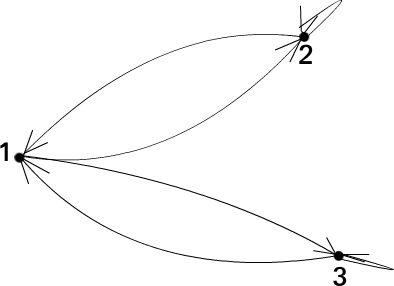
\includegraphics[width=.4\textwidth]{./pictures/14_5.png}
  \caption{Состояния и переходы цепи Маркова}
  \label{fig:145}
\end{figure}

Посчитаем вероятность того, что
\begin{enumerate}[label=\alph*)]
  \item \begin{gather*}
    P \left( X_1 = 2, X_2 = 2, X_3 = 2, X_4 = 1, X_5 = 3 \right) = \\
    = \frac{2}{5} \cdot \frac{1}{3} \cdot \frac{3}{4} \cdot \frac{3}{4} \cdot \frac{1}{4} \cdot
    \frac{2}{3} +
    \frac{1}{5} \cdot \frac{3}{4} \cdot \frac{3}{4} \cdot \frac{1}{4} \cdot \frac{2}{3} +
    \frac{2}{5} \cdot 0;
  \end{gather*}
  \item \begin{equation*}
    P \left( X_5 = 2, X_6 = 2 \; \middle| \; X_2 = 2 \right) =
    P \left( 2 \to \to \to 2 \to 2 \right) =
  \end{equation*}
  Надо перебрать все возможные варианты
  \begin{gather*}
    = P \left( 2 \to 2 \to 2 \to 2 \to 2 \right) + P \left( 2 \to 2 \to 1 \to 2 \to 2 \right) + \\
    + P \left( 2 \to 1 \to 2 \to 2 \to 2 \right).
  \end{gather*}
  Для каждого слагаемого нужно поперемножать вероятности.
\end{enumerate}

\addcontentsline{toc}{chapter}{Занятие 15. Цепи Маркова. Период состояний.
                                Инвариантное распределение.}
\chapter*{Занятие 15. Цепи Маркова. Период состояний. Инвариантное распределение.}

\addcontentsline{toc}{section}{Контрольные вопросы и задания}
\section*{Контрольные вопросы и задания}

\subsubsection*{Приведите определение цепи Маркова.}

Последовательность дискретных случайных величин $ \left\{ x_n \right\}_{n \geq 0}$
называется простой цепью Маркова (с дискретным временем), если
\begin{equation*}
  P \left( x_{n + 1} = i_{n + 1} \; \middle| \; x_n = i_n, \dotsc, x_0 = i_0 \right) =
  P \left( x_{n + 1} = i_{n + 1} \; \middle| \; x_n = i_n \right).
\end{equation*}

\subsubsection*{Что называется переходными вероятностями цепи Маркова?}

Матрица $P \left( n \right) $,
где $P_{ij} \left( n \right) = P \left( x_{n + 1} = i_{n + 1} \; \middle| \; x_n = i \right) $,
называется матрицей переходных вероятностей на $n$-м шаге.

\subsubsection*{Как вычисляются переходные вероятности цепи Маркова за $n$ шагов?}

Матрица переходных вероятностей за $n$ шагов однородной цепи Маркова есть $n$-я
степень матрицы переходных вероятностей за 1 шаг.

\subsubsection*{Запишите уравнение Колмогорова-Чепмена.}

$P \left( x_n - i_n \; \middle| \; x_0 = i_0 \right) =
  \left( P^n \right)_{i_0, i_n}$.

\subsubsection*{Опишите, как классифицируются состояния цепи Маркова.}

Группы состояний марковской цепи (подмножества вершин графа переходов),
которым соответствуют тупиковые вершины диаграммы порядка графа переходов,
называются эргодическими классами цепи.
Состояния, которые находятся в эргодических классах, называются существенными,
а остальные~---~несущественными.
Поглощающее состояние является частным случаем эргодического класса.
Тогда попав в такое состояние, процесс прекратится.

\subsubsection*{Что называется периодом состояния?}

Пусть дана однородная цепь Маркова с дискретным временем $ \left\{ x_n \right\}_{n \geq 0}$
с матрицей переходных вероятностей $P$.
В частности, для любого $n \in \mathbb{N}$,
матрица $P^n = \left( p_{ij}^{ \left( n \right) } \right) $
является матрицей переходных вероятностей за $n$ шагов.
Рассмотрим последовательность $p_{jj}^{ \left( n \right) }, \, n \in \mathbb{N}$.
Число
\begin{equation*}
  d \left( j \right) =
  gcd \left( n \in \mathbb{N} \; \middle| \; p_{jj}^{ \left( n \right) } > 0 \right),
\end{equation*}
где $gcd$ обозначает наибольший общий делитель, называется периодом состояния $j$.

\subsubsection*{Сформулируйте утверждение про периоды сообщающихся состояний.}

Периоды сообщающихся состояний совпадают:
$ \left( i \leftrightarrow j \right) \Rightarrow \left( d \left( i \right) =
  d \left( j \right) \right) $.

\subsubsection*{Сформулируйте теорему про ассимптотическое поведение переходных вероятностей
                $p_{ij}^{ \left( n \right) }$ при $n \to \infty $.}

При $n \to \infty $ матрица $P^n$ стремится к строго положительной матрице,
у которой все строки совпадают с равновесным распределением.

\subsubsection*{Дайте определение инвариантного распределения цепи Маркова.}

Будем предполагать,
что $ \sigma $-алгебра $ \varepsilon $ порождена счётным семейством подмножеств $E$.

Всякая $ \sigma $-конечная мера $ \pi \left( \cdot \right) $, удовлетворяющая уравнению
\begin{equation*}
  \pi \left( A \right) = \int \limits_{E} \pi \left( dx \right) P \left( x, A \right), \,
  A \in \varepsilon
\end{equation*}
и условию $ \pi \left( A \right) < \infty $ хотя бы для одного множества $A \in \varepsilon^+$,
называется инвариантной.

\addcontentsline{toc}{section}{Аудиторные задачи}
\section*{Аудиторные задачи}

\subsubsection*{15.4}

\textit{Задание.}
По виду матрицы переходных вероятностей проведите классификацию состояний соответствующей цепи
Маркова и найдите её инвариантное распределение.
\begin{enumerate}[label=\alph*)]
  \item \begin{equation*}
    P =
    \begin{bmatrix}
      0 & 0 & \frac{1}{3} & \frac{1}{3} & \frac{1}{3} \\
      0 & \frac{1}{3} & \frac{1}{3} & \frac{1}{3} & 0 \\
      \frac{1}{4} & \frac{1}{4} & \frac{1}{4} & \frac{1}{4} & 0 \\
      0 & 0 & 0 & \frac{1}{2} & \frac{1}{2} \\
      0 & 0 & 0 & \frac{1}{2} & \frac{1}{2}
    \end{bmatrix};
  \end{equation*}
  \item \begin{equation*}
      P =
      \begin{bmatrix}
        0 & 0 & 0 & \frac{1}{2} & \frac{1}{2} \\
        0 & \frac{1}{2} & \frac{1}{2} & 0 & 0 \\
        0 & 1 & 0 & 0 & 0 \\
        0 & 1 & 0 & 0 & 0 \\
        0 & 0 & 0 & 1 & 0
      \end{bmatrix}.
  \end{equation*}
\end{enumerate}

\textit{Решение.}
\begin{enumerate}[label=\alph*)]
  \item $ \pi = \left( \pi_1, \pi_2, \pi_3, \pi_4, \pi_5 \right) $.

  Инвариантное распределение можно найти из условия $ \pi P = \pi $.

  Получим систему уравнений
  \begin{equation*}
    \begin{cases}
      \frac{ \pi_3}{4} = \pi_1, \\
      \frac{ \pi_2}{3} + \frac{ \pi_3}{4} = \pi_2, \\
      \frac{ \pi_1}{3} + \frac{ \pi_2}{3} + \frac{ \pi_3}{4} = \pi_3, \\
      \frac{ \pi_1}{3} + \frac{ \pi_2}{3} + \frac{ \pi_3}{4} + \frac{ \pi_4}{2} + \frac{ \pi_2}{5} =
      \pi_4, \\
      \frac{ \pi_1}{3} + \frac{ \pi_4}{2} + \frac{ \pi_5}{2} = \pi_5, \\
      \pi_1 + \pi_2 + \pi_3 + \pi_4 + \pi_5 = 1,
    \end{cases}
  \end{equation*}
  где последнее уравнение возникло из-за того, что это распределение.

  Это система однородных уравнений.

  Решений не больше одного.
  Теперь найдём это решение.

  $ \pi_3 = 4 \pi_1$.
  Подставим это во второе уравнение
  \begin{equation*}
    \frac{ \pi_2}{3} + \pi_1 = \pi_2 \Rightarrow
    \frac{2 \pi_2}{3} = \pi_1 \Rightarrow
    \pi_2 = \frac{3 \pi_1}{2}.
  \end{equation*}

  Получим уравнение для нахождения $ \pi_1$, то есть
  \begin{equation*}
    \frac{ \pi_1}{3} + \frac{ \pi_1}{2} + \pi_1 =
    4 \pi_1.
  \end{equation*}

  Приведём подобные
  \begin{equation*}
    \frac{5 \pi_1}{6} = 3 \pi_1 \Rightarrow \pi_1 = 0.
  \end{equation*}

  Отсюда следует, что $ \pi_2 = 0, \, \pi_3 = 0$.

  Остаётся 2 уравнения
  \begin{equation*}
    \begin{cases}
      \frac{ \pi_4}{2} + \frac{ \pi_5}{2} = \pi_4 \Rightarrow \pi_4 = \pi_5, \\
      \pi_4 + \pi_5 = 1.
    \end{cases}
  \end{equation*}

  Отсюда
  \begin{equation*}
    \pi_4 =
    \pi_5 =
    \frac{1}{2}.
  \end{equation*}

  Ответ: инвариантное распределение
  \begin{equation*}
    \left( 0, 0, 0, \frac{1}{2}, \frac{1}{2} \right).
  \end{equation*}
  Почему так получается?
  Посмотрим, какие есть переходы в этой цепи.
  Есть 5 состояний (рис. \ref{fig:154}).

  \begin{figure}[h!]
    \centering
    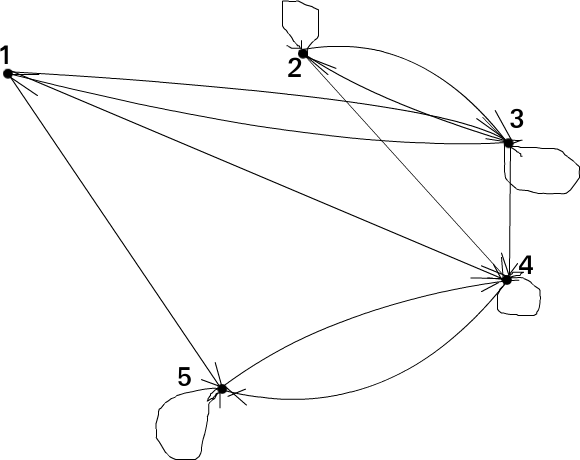
\includegraphics[width=.4\textwidth]{./pictures/15_4.png}
    \caption{Состояния и переходы цепи Маркова}
    \label{fig:154}
  \end{figure}

  $4 \leftrightarrow 5$~---~существенные.

  $1 \leftrightarrow 2 \leftrightarrow 3$~---~несущественные.

  Инвариантное распределение не может иметь положительную вероятность на несущественном состоянии.
  \item Найдём инвариантное распределение для такой матрицы (рис. \ref{fig:1541}).

  \begin{figure}[h!]
    \centering
    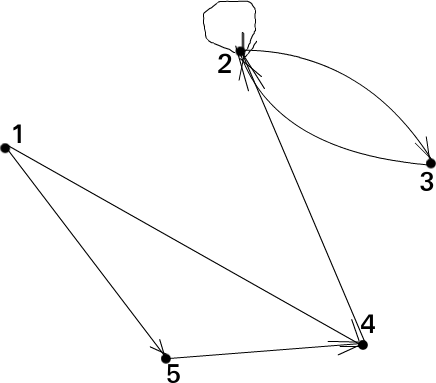
\includegraphics[width=.4\textwidth]{./pictures/15_4_1.png}
    \caption{Состояния и переходы цепи Маркова}
    \label{fig:1541}
  \end{figure}

$2 \leftrightarrow 3$.

Состояния $1, 4, 5$~---~несущественные.

Это значит, что
\begin{equation*}
  \pi \; : \;
  \left( 0, \frac{1}{3}, \frac{2}{3}, 0, 0 \right).
\end{equation*}

Только 2 состояния существенные, значит, уравнения будут такими:
\begin{equation*}
  \begin{cases}
    \frac{ \pi_2}{2} + \pi_3 = \pi_2, \\
    \frac{ \pi_2}{2} = \pi_3, \\
    \pi_2 + \pi_3 = 1.
  \end{cases}
\end{equation*}
\end{enumerate}

\subsubsection*{15.5}

\textit{Задание.}
Найдите инвариантное распределение симметрического блуждания на $ \left[ 0, N \right] $
с поглощением на концах.

\textit{Решение.}
$ \left\{ X_n \right\}_{n \geq 0}$~---~это симметричное случайное блуждание с поглощением в точках
$ \left\{ 0, N \right\} $.
Представим себе, как такая цепь движется.
Цепь принимает значения в отрезке (рис. \ref{fig:155}).

\begin{figure}[h!]
  \centering
  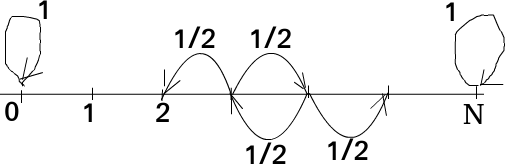
\includegraphics[width=.4\textwidth]{./pictures/15_5.png}
  \caption{Состояния и переходы цепи Маркова}
  \label{fig:155}
\end{figure}

Напишем матрицу переходных вероятностей
\begin{equation*}
  P =
  \begin{bmatrix}
    1 & 0 & 0 & 0 & \dotsc & 0 \\
    \frac{1}{2} & 0 & \frac{1}{2} & 0 & \dotsc & 0 \\
    \dotsc & \dotsc & \dotsc & \dotsc & \dotsc & \dotsc & \\
    0 & 0 & 0 & 0 & \dotsc & 1
  \end{bmatrix}.
\end{equation*}

Как тут будет выглядеть инвариантное распределение?

Все состояния кроме концов отрезка несущественные.
Это означает, что $ \pi_i = 0, \, i \neq 0, N$.

Получаем систему уравненеий
\begin{equation*}
  \begin{cases}
    \pi_1 = \pi_1, \\
    \pi_N = \pi_N, \\
    \pi_1 + \pi_N = 1.
  \end{cases}
\end{equation*}

Это означает, что у нас только одно уравнение на эти вероятности.

Тут инвариантных распределений бесконечно много.
Любое инвариантное распределение имеет вид $ \left( \pi_1, 0, 0, 0, \dotsc, 0, 1 - \pi_1 \right) $.

\addcontentsline{toc}{section}{Домашнее задание}
\section*{Домашнее задание}

\subsubsection*{15.12}

\textit{Задание.}
По виду матрицы переходных вероятностей проведите классификацию состояний соответственной цепи
Маркова и найдите его инвариантное распределение.
\begin{equation*}
  P =
  \begin{bmatrix}
    \frac{1}{2} & 0 & \frac{1}{2} & 0 & 0 \\
    0 & \frac{1}{2} & 0 & 0 & \frac{1}{2} \\
    0 & 0 & 0 & 1 & 0 \\
    \frac{1}{3} & 0 & \frac{1}{3} & \frac{1}{3} & 0 \\
    \frac{1}{2} & 0 & 0 & 0 & \frac{1}{2}
  \end{bmatrix}.
\end{equation*}

\textit{Решение.}
$ \pi = \left( \pi_1, \pi_2, \pi_3, \pi_4, \pi_5 \right) $.

Инвариантное распределение можно найти из условия $ \pi P = \pi $.

Получим систему уравнений
\begin{equation*}
  \begin{cases}
    \frac{ \pi_1}{2} + \frac{ \pi_4}{3} + \frac{ \pi_5}{2} = \pi_1, \\
    \frac{ \pi_2}{2} = \pi_2, \\
    \frac{ \pi_1}{2} + \frac{ \pi_4}{3} = \pi_3, \\
    \pi_3 + \frac{ \pi_4}{3} = \pi_4, \\
    \frac{ \pi_2}{2} + \frac{ \pi_5}{2} = \pi_5, \\
    \pi_1 + \pi_2 + \pi_3 + \pi_4 + \pi_5 = 1,
  \end{cases}
\end{equation*}
где последнее уравнение возникло из-за того, что это распределение.

Это система однородных уравнений.

Решений не больше одного.
Теперь найдём это решение.

$ \pi_2 = 0$.
Подставим это в пятое уравнение
\begin{equation*}
  \frac{ \pi_5}{2} = \pi_5, \Rightarrow
  \pi_5 = 0.
\end{equation*}

Остаются уравнения
\begin{equation*}
  \begin{cases}
    \frac{ \pi_1}{2} + \frac{ \pi_4}{3} = \pi_1, \\
    \frac{ \pi_1}{2} + \frac{ \pi_4}{3} = \pi_3, \\
    \pi_3 + \frac{\pi_4}{3} = \pi_4, \\
    \pi_1 + \pi_3 + \pi_4 = 1.
  \end{cases}
\end{equation*}

Из первого уравнения получаем
\begin{equation*}
  \frac{ \pi_4}{3} = \pi_1 - \frac{ \pi_1}{2} = \frac{ \pi_1}{2} \Rightarrow
  \pi_4 = \frac{3 \pi_1}{2}.
\end{equation*}
Подставим во второе уравнение
\begin{equation*}
  \frac{ \pi_1}{2} + \frac{ \pi_1}{2} =
  \pi_3 = \pi_1.
\end{equation*}

Подставим в последонее уравнение
\begin{equation*}
  \pi_1 + \pi_1 + \frac{3 \pi_1}{2} = 1 \Rightarrow
  2 \pi_1 + \frac{3 \pi_1}{2} = 1 \Rightarrow
  \frac{7 \pi_1}{2} = 1 \Rightarrow
  \pi_1 = \frac{2}{7} \Rightarrow
  \pi_4 = \frac{3}{2} \cdot \frac{2}{7} = \frac{3}{7}.
\end{equation*}

Ответ: инвариантное распределение:
\begin{equation*}
  \left( \frac{2}{7}, 0, \frac{2}{7}, \frac{3}{7}, 0 \right).
\end{equation*}

Почему так получилось?
Посмотрим, какие есть переходы в этой цепи?

Есть 5 состояний (рис. \ref{fig:1512}).

\begin{figure}[h]
  \centering
  \includestandalone[mode=buildnew]{./pictures/15_12}
  \caption{Состояния и переходы цепи Маркова}
  \label{fig:1512}
\end{figure}

$1 \leftrightarrow 3 \leftrightarrow 4$~---~существенные.

$2, 5$~---~несущественные.

Инвариантное распределение не может иметь положительную вероятность на несущественном состоянии.

\subsubsection*{15.13}

\textit{Задание.}
Найдите инвариантное распределение симметрического блуждания на $ \left[ 0, N \right] $
\begin{enumerate}[label=\alph*)]
  \item с отражением на концах;
  \item с отражением на одном из концов и поглощением на другом.
\end{enumerate}

\textit{Решение.}
\begin{enumerate}[label=\alph*)]
  \item $ \left\{ X_n \right\} $~---~симметрическое блуждание с отражением в точках
  $ \left\{ 0, N \right\} $.

  Представим себе, как такая цепь движется.
  Цепь принимает значения в отрезке (рис. \ref{fig:1513}).

  \begin{figure}[h]
    \centering
    \includestandalone[mode=buildnew, width=.9\textwidth]{./pictures/15_13}
    \caption{Состояния и переходы цепи Маркова}
    \label{fig:1513}
  \end{figure}

  Напишем матрицу переходных вероятностей
  \begin{equation*}
    P =
    \begin{bmatrix}
      0 & 1 & 0 & 0 & \dotsc & 0 \\
      \frac{1}{2} & 0 & \frac{1}{2} & 0 & \dotsc & 0 \\
      0 & \frac{1}{2} & 0 & \frac{1}{2} & \dotsc & 0 \\
      \dotsc & \dotsc & \dotsc & \dotsc & \dotsc & \dotsc \\
      0 & 0 & 0 & 0 & \dotsc & 0
    \end{bmatrix}.
  \end{equation*}

  Как тут будет выглядеть инвариантное распределение?

  Получается система уравнений
  \begin{equation*}
    \begin{cases}
      \frac{1}{2} \cdot \pi_1 = \pi_0, \\
      \pi_0 + \frac{1}{2} \cdot \pi_2 = \pi_1, \\
      \frac{1}{2} \cdot \pi_1 + \frac{1}{2} \cdot \pi_3 = \pi_2, \\
      \frac{1}{2} \cdot \pi_2 + \frac{1}{2} \cdot \pi_4 = \pi_3, \\
      \dotsc, \\
      \frac{1}{2} \cdot \pi_{N - 1} = \pi_N, \\
      \pi_0 + \pi_1 + \dotsc + \pi_N = 1.
    \end{cases}
  \end{equation*}

  Из первого уравнения $ \pi_1 = 2 \pi_0$.

  Подставим это во второе уравнение
  \begin{equation*}
    \pi_0 + \frac{1}{2} \cdot \pi_2 = 2 \pi_0 \Rightarrow
    \pi_0 = \frac{1}{2} \cdot \pi_2 \Rightarrow
    \pi_2 = 2 \pi_0.
  \end{equation*}

  Подставим это в третье уравнение
  \begin{equation*}
    \pi_0 + \frac{1}{2} \cdot \pi_3 = 2 \pi_0 \Rightarrow
    \pi_0 = \frac{1}{2} \cdot \pi_3 \Rightarrow
    \pi_3 = 2 \pi_0.
  \end{equation*}

  Таким образом, $ \pi_1 = \pi_2 = \dotsc = \pi_{N - 1} = 2 \pi_0, \, \pi_N = \pi_0$.

  Подставим это в последнее уравнение $ \pi_0 + 2 \pi_0 \left( N - 1 \right) + \pi_0 = 1$.

  Приведём подобные
  \begin{equation*}
    N \pi_0 = \frac{1}{2}.
  \end{equation*}

  Отсюда находим, что
  \begin{equation*}
    \pi_0 =
    \frac{1}{2N} =
    \pi_N.
  \end{equation*}

  Значит,
  \begin{equation*}
    \pi_1 =
    \dotsc =
    \pi_{N - 1} =
    \frac{1}{N}.
  \end{equation*}

  Инвариантное распределение имеет вид
  \begin{equation*}
    \left( \frac{1}{2N}, \frac{1}{N}, \dotsc, \frac{1}{N}, \frac{1}{2N} \right);
  \end{equation*}
  \item последовательность случайных величин
  $ \left\{ X_n \right\}_{n \geq 0}$~---~симметричное случайное блуждание с поглощением в точке
  $ \left\{ 0 \right\} $ и отражением в точке $ \left\{ N \right\} $.
  Представим себе, как такая цепь движется.
  Цепь принимает значения на отрезке (рис. \ref{fig:15131}).

  \begin{figure}[h]
    \centering
    \includestandalone[mode=buildnew, width=.9\textwidth]{./pictures/15_13_1}
    \caption{Состояния и переходы цепи Маркова}
    \label{fig:15131}
  \end{figure}

  Напишем матрицу переходных вероятностей
  \begin{equation*}
    P =
    \begin{bmatrix}
      1 & 0 & 0 & 0 & \dotsc & 0 \\
      \frac{1}{2} & 0 & \frac{1}{2} & 0 & \dotsc & 0 \\
      \dotsc & \dotsc & \dotsc & \dotsc & \dotsc & \dotsc \\
      0 & 0 & 0 & 0 & \dotsc & 0
    \end{bmatrix}.
  \end{equation*}

  Как тут будет выглядеть инвариантное распределение?

  Все состояния кроме $ \left\{ 0 \right\} $ несущественные.
  Это означает, что
  \begin{equation*}
    \pi_i = 0, \,
    i \neq 0.
  \end{equation*}

  Получаем систему уравнений
  \begin{equation*}
    \begin{cases}
      \pi_1 = \pi_1, \\
      \pi_1 = 1.
  \end{cases}
  \end{equation*}

  Тут инвариантное распределение имеет вид $ \left( 1, 0, 0, 0, \dotsc, 0, 0 \right) $.
\end{enumerate}


\end{document}
